\documentclass[12pt]{report}
\usepackage{cmap} % to make pdf searchable, puts text underneath ligatures
\usepackage[T1]{fontenc}
\usepackage[utf8]{inputenc}
\usepackage{graphicx} 
\usepackage[a4paper,  margin=3cm]{geometry}
\usepackage[main=british, ngerman]{babel}
\usepackage{wrapfig}
\usepackage[autostyle=true,english=british]{csquotes}
 %  \MakeAutoQuote{‘}{’}
\usepackage{amsmath,amssymb}
\usepackage{mathbbol}%if cardinality or unit is needed
\usepackage{tabularx}
\usepackage{longtable}%multiple pages table 
\usepackage{multirow}
\usepackage{booktabs}
\usepackage{pdflscape}
\usepackage{adjustbox}
\usepackage{wrapfig}
\usepackage[font={footnotesize},labelfont=bf]{subcaption}
\usepackage{array}
\usepackage[position=bottom,tableposition=bottom,font={footnotesize},labelfont=bf, singlelinecheck=false,
    format=plain]{caption}
\usepackage{float} % fixieren von grafiken
\usepackage[backend=biber, style=numeric, citestyle=numeric, sorting=nty,maxbibnames=5]{biblatex}
%changed cite style to nature from bwl fu because of PhD thesis in Netz' group
\usepackage[position=bottom,tableposition=bottom,font={footnotesize},labelfont=bf]{caption}
\captionsetup[table]{justification=centering}
\usepackage{chngpage}
\usepackage{titling}
\usepackage{placeins}
\usepackage{sidecap}
\usepackage{hyperref} %always put as last package!

\newcommand{ \aladincitation } [1] { \citeauthor{#1}, \citefield{#1}{title}, \citefield{#1}{journaltitle}, \citeyear{#1}. \newline} 



\author{Magdalena Haselsteiner}


\date{February 2017}
\addbibresource{master.bib}

\renewcommand{\arraystretch}{1.5}
\setlength{\parindent}{0pt}

\begin{document}
%\pagestyle{empty}
\setlength\parindent{0pt}
\begin{titlepage}
\pagenumbering{gobble} 

\centering {  {\Large\textbf{Master's Thesis}}\\ \vspace{4 cm} \Huge Application of Ensemble Prediction on a Visibility Parametrization based on Mie Scattering Theory}\\
        \vspace{1.5 cm}
        {\Large by Magdalena Elisabeth Haselsteiner}\\
        \vspace{4.5cm}
        \centering \textbf{ {\large Freie Universität Berlin\\ Fachbereich Physik}}
        
		\vspace{3cm}
        \begin{adjustbox}{left=30cm}
   

	    \end{adjustbox}
	    \vspace{\fill}
	
        \hspace{-3cm}
	   \begin{minipage}[B]{0.3\textwidth }
	   
	        
\includegraphics[width=\textwidth] {graphics/logos/ZAMGhead.jpg}
	     
	       \end{minipage}
     \hspace{2.5cm}
   \begin{minipage}[B]{0.5\textwidth }

	        
\includegraphics[width=\textwidth ] {graphics/logos/FULogo.jpg}
	       
	         \end{minipage}
     
\pagebreak

	\begin{tabular}{l l}
	        Title & Application of Ensemble Prediction\\[-0.1cm]
	            &  on a Visibility Parametrization \\[-0.1cm]
	            & based on Mie Scattering Theory\\[0.3cm]
		    Author &  Magdalena Elisabeth Haselsteiner\\
		    Matriculation Number & 4973395\\
		    Date of Birth & 27.5.1992, Korneuburg, Austria\\
		    University/Department & Free University Berlin, Department of Physics\\
		    Course of Studies & Master studies, Physics\\
		    $1^{st}$ Reviewer & Prof. Dr. Roland Netz\\
		    $2^{nd}$ Reviewer & PD. Dr. Stefanie Russ\\
		    In Cooperation with & Zentralanstalt für Meteorologie und Geodynamik\\
		    Date of Submission & 08.05.2018 \\
		\end{tabular}
\end{titlepage}

\newpage
{\parskip=0em
\tableofcontents}
\newpage
\listoffigures
\newpage
\pagenumbering{arabic}
\begin{abstract}
    
    This  Master's thesis aims to describe and evaluate a new parametrization for forecasting visibility within numerical weather prediction. The parametrization represents Mie scattering on atmospheric aerosols and hydrometeors and is implemented in a numerical weather prediction model, written in Fortran.\\
    To examine the uncertainty in the parametrization and its effects, ensemble prediction is used. A new local perturbation scheme is introduced. For the verification of the visibility forecast, a logarithmic score  and the Ranked Probability Skill Score are chosen to evaluate the predicted values against the observed values, which were taken at meteorological observation sites on the domain of the forecast.\\
    The new parametrization in its current implementation outperforms the reference parametrization only in a few cases. However, we have reason to believe that further improvements the aerosol scheme will result in a significant increase of performance. The new perturbation scheme enhanced the ensemble skill remarkably in the whole verification period. The scheme can also be generalized and applied to other parametrizations or model parts of similar kind.
        
\end{abstract}
\chapter{Introduction} 

The humankind has always been exposed to nature, especially the weather.  Change of climate or extreme weather events have erased whole cultures from our planet, so no wonder that since the very early days of humanity, we observed our atmosphere, tried to find patterns and predict upcoming weather events.  Already in 340 BC Aristotle wrote the `Meteorologica', which can be seen as the very first documented structured approach to weather forecasting.
For a long time, meteorology was a purely empirical science, because there was no deeper understanding of the underlying physical processes. It was only at the beginning of the 20th century when \citeauthor{abbe1901physical} \cite{abbe1901physical} was the first one to draw the connection between large scale atmospheric processes and physics.
From there on we have come a very long way to where we are today. Because weather prediction is an overlap of physics, mathematics and, more recently, computer science, meteorology has evolved hand in hand with those fields.
Due to enhancements in above-mentioned disciplines, forecasts improved rapidly in the last 40 years: one day per decade. Meaning that today the accuracy of a prediction four days ahead is the same as the accuracy of a prediction three days ahead ten years ago \parencite{bauer2015quiet}. Nevertheless researchers in universities, private enterprises, governmental and military institutions are still trying to push it further. This is because the weather affects us in so many different ways, that having skilful predictions caters to different, sometimes even opposed, needs and interests. It can be a major contributor to sustain peace and stability for humanity as a whole, especially because of its role in agriculture and food production, and it can also be a valuable tool for the prevention of economic losses due to weather events and for the management of natural disasters \cite{webster2013meteorology}.\\ \\
The basis of modern weather forecast is to  mathematically describe the atmosphere as a turbulent fluid, using thermodynamics and fluid mechanics, and to solve the corresponding equations numerically \cite{coiffier2011fundamentals, batkai2016mathematical, phillips1960problem}.\\
The atmosphere is an intrinsically chaotic system and therefore it is very challenging to model and predict its behaviour \cite{lorenz1963deterministic}. It is  crucial to take the full range of possible initial conditions into account by modelling different possible scenarios of one case. This requires enormous computational power and sophisticated parallelization techniques \cite{batkai2016mathematical, leutbecher2008ensemble}. The improvement of computational facilities in recent years enhanced accuracy of the models, which caused Numerical Weather Prediction (NWP) to become the main area of research in meteorology and it is evolving rapidly. \\ \\
The spatial and temporal resolution is constantly getting higher and so the NWP models need to be adapted \cite{aladin1, theis_hense_damrath_2005}. With each improvement in the resolution more processes can be calculated explicitly, instead of using inaccurate empirically gained representations, and as a result, the contribution of model error is going down \cite{bauer2015quiet}. Besides the efforts of adapting models to a higher resolution the second area of focus of research in NWP is ensemble forecasting: to determine and evaluate the uncertainty of the forecast. Therefore, different scenarios, of the same prediction are simulated and the output of the whole ensemble is analysed. The statistics obtained from the ensemble provide insight about what scenario can be expected with the corresponding probability \cite{batkai2016mathematical}.
One of the main contributors to model uncertainty are parametrizations \cite{ollinaho2017towards, leutbecher2008ensemble}. 
Parametrizations are needed, because a large number of different complex physical processes leads to a single atmospheric state \cite{coiffier2011fundamentals}. Most modern NWP models use a temporal resolution of approximately 60 seconds. Due to limited computational capacities it is impossible to simulate all the underlying physical processes explicitly, for every time step for which the atmospheric state is determined. Hence, many of these simulations are replaced by mainly empirically gained representations, the parametrizations.
Paired with the uncertainties of the initial state and the chaotic nature of the atmosphere, the use of statistical methods becomes inevitable \cite{palmer2009stochastic, buizza1999stochastic, leutbecher2008ensemble}.\\
Depending on the purpose of the forecast, different variables of NWP models are of interest: Obviously the thermodynamic state variables, but often also additional ones e.g. accumulated precipitation for estimating the risk of flooding \cite{theis_hense_damrath_2005}, or sunshine duration to plan, when to carry out certain tasks in agriculture.\\
In the course of this Master's thesis, we are interested in predicting horizontal visibility, where especially for air traffic there is a demand for reliable forecasts.
Visibility is a measure for the shortest horizontal distance for which an object is still visible to a human observer, considering all directions \parencite{clark2008prediction, WMO, price2007advanced}.
It is effected by a great number of non-linear processes like precipitation and radiative processes.
Most parametrizations implemented in operational models are simple functions of the relative humidity, gained by fitting to measurement data, and can be evaluated analytically  \cite{gultepe2010probabilistic}.
The coefficients of the fit functions and even the function types, can vary vastly between different parametrizations, because they cannot be directly related to any physical process.
The dominating physical process that impacts visibility is Mie scattering, which is the scattering of plane electromagnetic waves on a sphere, for cases where the radius of the sphere and the wavelength of the incoming light have about the same size range \parencite{mie1908beitrage}. For sunlight different atmospheric particles satisfy this condition \parencite{wallace2006atmospheric}. Hence, the most accurate way of predicting visibility should be to resolve Mie scattering on hydrometeors and aerosols directly.
But because the spatial and temporal distribution of them is difficult to predict, there is a high level of overall uncertainty when trying to predict visibility by the use of Mie theory. As mentioned, probabilistic forecasts in general and ensemble prediction in particular can help to get meaningful results, even when the associated uncertainty is high.
Motivated by other attempts of probabilistic visibility forecasts \cite{chmielecki2011probabilistic, Roquelaure}, we combined ensemble methods and the theory of atmospheric scattering to a new scheme for probabilistic visibility prediction. 
This work presents and evaluates a new parametrization of visibility, based on Mie scattering theory, and how ensemble forecasting can be applied to predict visibility. It was carried out in cooperation with `Zentralanstalt für Meteorologie und Geodynamik' \cite{zamg}, the Austrian meteorological service.\\ \\
The necessary background theory to understand the basics of numerical weather prediction, the framework of this study, is provided in Chapter \ref{sec:bt}. In addition, the definition and mathematical derivation of visibility is provided and Mie theory is revised.\\
In Chapter \ref{sec:model} the model we used, is described, with special focus on the pattern generator for stochastic perturbations. The details of the new visibility parametrization and the benchmark  parametrizations are explained in Chapter \ref{sec:param}. Methods and set-up, including the evaluation strategies are the subject of Chapter \ref{sec:methods}. Then the results are presented and discussed in Chapter \ref{sec:results}. Finally, an outlook on potential future studies and concluding remarks, about strengths and weaknesses of the visibility prediction method is given in Chapter \ref{sec:con_n_out}.\\
\\
All used variables and abbreviations are listed in Appendix \ref{sec:tabelappendix} in Table \ref{tab: variables} and Table \ref{tab:abbrivitations}.




\chapter{Background Theory}
\label{sec:bt}
\section{Numerical Weather Prediction Models}
Numerical Weather Prediction models evolved from the approach to describe the atmosphere in terms of more general physical laws. In this section the basic assumptions and equations for NWP models are outlined according to \citeauthor{coiffier2011fundamentals} \cite{coiffier2011fundamentals}.\\ \\
The core of every NWP model is based upon the `Primitive Equations' which are a form of the Navier-Stokes equations  describing: 
\begin{itemize}
\item{Momentum}
\item{Mass transportation}
\item{Energy balance}
\end{itemize}
 of a fluid \parencite{phillips1960problem}.
\subsection{Primitive Equations}
The following equations describe the dynamics of the atmosphere and are the core of every NWP Model.\\
\subsubsection{Equation of Momentum}
Here the acceleration of a frictionless flow of a Newtonian fluid is described. The equation is derived by taking the time derivative of the equation of momentum of a parcel of air
    \begin{equation}
        \frac{d \vec{v}}{dt} = -2 \vec{\Omega} \times \vec{v} - \frac{1}{\rho} \vec{\nabla} p - \vec {\nabla} \Phi + \vec{F} \quad ,
        \label{eq:Navier-Stokes}
    \end{equation}
where $\vec{v}$ denotes the wind velocity, $\vec{\Omega}$  the angular velocity of the Earth, $ \rho$ the density of air, $p$ the pressure, $\Phi$ the  geopotential and  $\vec{F}$ dissipative forcing. 

\subsubsection{Equation of State}
The ideal gas law is used here. Equation \ref{eq:idealgas} is the simplest equation of state of a gas and describes the constant relation of pressure $p$, density $\rho$ and temperature $T$ in  an ideal gas, which is proportional to the gas constant $R$.
    \begin{equation}
        p = \rho R T
    \label{eq:idealgas}    
    \end{equation}    

\subsubsection{Conservation of Energy}
   Equation \eqref{eq:consener} is derived from the First Law of Thermodynamics. 
    \begin{equation}
        \frac{dT}{dt} = \frac{R}{C_{p}} \frac{T}{p} \frac{dp}{dt} + \frac{1}{C_{p} }\frac{dQ}{dt}
    \label{eq:consener}
    \end{equation}
   The nomenclature is the same as for Equation \eqref{eq:Navier-Stokes} and \eqref{eq:idealgas}. The specific heat of air at a constant pressure $p$ is denoted by $C_{p}$ and the heat by $Q$.

\subsubsection{Continuity Equation}
In general the continuity equation describes the change in time of the density of a quantity that is preserved, which in this case is mass.
    \begin{equation}
        \frac{d \rho}{ dt} = - \rho \vec{\nabla} \vec{v}
    \label{eq:continuity}    
    \end{equation}
The nomenclature remains the same as in Equation \eqref{eq:Navier-Stokes}.
\subsubsection{Water Vapour Equation}
The water vapour equation is usually not seen as part of the primitive equations, but considered in almost all atmospheric models.
    \begin{equation}
        \frac{dq_{\mathrm{spec}}}{dt} = M 
    \label{eq:consvap}    
    \end{equation}
Here $q_{\mathrm{spec}}$ denotes the specific humidity and $M$ the source or sink term for humidity. 

\subsection{Approximations}
\label{subsec:approx}
Depending on the model, different approximations need to be made to reduce the system of equations to a more easily solvable problem.
The most common one is the so-called traditional meteorological approximation. It consists of:
    \begin{itemize}
        \item{The assumption that the gravitational acceleration is constant}
        \item{The assumption that the Earth is a perfect sphere}
        \item {The replacement of the Earth's angular velocity vector $\vec {\Omega}$ by its vertical component: $\vec {\Omega} = \Omega \vec{e_{r}}sin \phi = \frac{f}{2} \vec{e_{r}} $, where $\phi$ denotes the latitude}
    \end{itemize}
Setting $\frac{f}{2} \vec{e_{r}}$ to $\Omega$ is necessary, to be able to separate the wind vector into a vertical and a horizontal component.
$F$, $\frac{dQ}{dt}$ and $M$ are source and sink terms that depend on parametrizations and scale of the model. For an adiabatic, frictionless and water vapour conserving atmosphere their contributions become 0.

A very common approximation is to assume hydrostatic balance in a model. Meaning, 
\begin{equation}
    \frac{\partial p}{ \partial z } = \rho g
    \label{eq:hydrobal}
\end{equation} 
needs to be satisfied.
Equation \eqref{eq:hydrobal} implies, that there are no vertical winds and is therefore not suitable for models that use a fine mesh size, because for many small scale processes, e.g. convection and turbulence, vertical winds are essential. For that reason, most limited area models (e.g. AROME \cite{gmd-2017-103}) are non-hydrostatic. However, for models with large mesh sizes, mostly global models, this simplification can help reducing the computation time and still provides meaningful results.

\subsection{System of Coupled Partial Differential Equations}
To get a system of coupled partial differential equations (PDEs) that can be solved numerically, we start by taking Equations \eqref{eq:Navier-Stokes}, \eqref{eq:idealgas}, \eqref{eq:consener} and \eqref{eq:continuity} replacing the wind velocity $\vec{v}$ by a horizontal wind vector $ \vec{V} $ and a vertical wind component $w$ times the radial unit vector $\vec{e_{r}}$ as $\vec{v} = \vec{V} + w \vec{e_{r}} $. The source and sink terms are neglected for now.
Together with the approximations we introduced in Subsection \ref{subsec:approx} and by setting $\frac{R}{C_{p}}=\kappa$, what in meteorology if referred to as `Poisson constant', the system of PDEs  takes the form:
\vspace{1cm}
\begin{equation}
    \frac{d\vec{V}}{dt} = -f \vec{e_{r}} \times \vec{V} - \frac{RT}{p}\vec{\nabla}_{\mathrm{h}} p
\end{equation}
\begin{equation}
   \frac{dw}{dt} = - \frac{RT}{p} \frac{\partial p}{\partial z} -g 
\end{equation}
\begin{equation}
    \frac{dT}{dt} = \kappa \frac{T}{p}\frac{d p}{d t}
\end{equation}
\begin{equation}
    \frac{dp}{dt} = - \frac{p}{ 1 - \kappa} \left( \vec{\nabla}_{\mathrm{h}} \vec{V} + \frac{dw}{dz} \right)
\end{equation}
\vspace{1cm}\\
The sub-scripted h in the differential operators denotes only the horizontal components of the operator.
These PDEs need to be solved and integrated for each time step, to get the  current values of the variables $\vec{V}, w, T$ and $ p$. Then, the so-called `parametrized tendencies' are added to the current value of the variables. The parametrized tendencies relate to source and sink terms and are the sum of the corresponding physics parametrization. Those parametrizations represent physical properties and processes that were neglected for simplification of the system of equations, when setting up the system of PDEs and are calculated separately at each time step. By the use of this iterative method, the atmospheric system can be evolved in time and predictions for the future can be made.\\
The best way of solving the system of PDEs varies depending on purpose and scale of the model.\\
The two most common methods to numerically solve those equations in numerical weather prediction are:
\begin{itemize}
    \item{Spectral Method}
    \item{Finite Differences Method}
\end{itemize}
The spectral method is only one approach of a whole set of numerical methods, which are all based on the idea of expanding the solutions in terms of base functions. The finite element and finite volume method are also of the same nature but not discussed here, because they are only of minor importance in NWP modelling \cite{batkai2016mathematical}.
In the spectral method the solutions are assumed to be global wave functions, defined on the whole domain. The main advantage is that the derivatives can be obtained analytically.\\
The method of finite differences, on the other hand, is a local approach. It uses the differential quotient on a discrete grid to approximate the derivative. Meaning that the numerical procedure only uses local values. Consequently, finite differences solutions lack the capability of reflecting certain global characteristics of a function accurately, but they only require local values at a time for the calculation. Thus, the finite differences method is increasingly popular, because it can make use of very efficient parallelization procedures, where the grid space is divided into sub-domains \cite{batkai2016mathematical}.\\ 
Nevertheless, the spectral method is still more common in global models, resulting from the fact that the spherical harmonics can be used as the global wave functions \cite{batkai2016mathematical, coiffier2011fundamentals}. They are the eigenfunctions of the angular dependent component of the Laplace operator and very suitable ansatz functions on a spherical domain. On other domains it is often not possible to find appropriate global wave functions and the bad approximation results in large trade-offs in numeric accuracy. These drawbacks led to the wide-spread use of the finite differences method in limited area models. \\

%Einleitung ueber Chaos und Lyapunov Exponent

\section{Ensemble Prediction}
\subsection{The Atmosphere's Chaotic Nature}

%Introduction to the Theory of Stability Buch zum Nachschalgen
%wichtigkeit vohrersagrbarkeit und zuverlaessigkeit qunatifizieren
\citeauthor{poincare1897forme} was the first one to describe a chaotic system, namely the solar system. When he tried to predict the planetary orbits, he started with the simplest case, a system of two large bodies, rotating each other, and discovered that even a very small third body can destabilize the system  \cite{poincare1897forme}.
Then a long time passed, before Edward Lorenz, who is often referred to as the father of chaos theory, published his discovery, revealing why the difficulties of reliable meteorological forecasts are inherent:
Atmospheric dynamics is highly sensitive to even the smallest changes in the initial and boundary conditions. A small error can propagate and be amplified through non-linear feedback processes to a magnitude much higher than its initial value. If that is the case, completely different scenarios emerge after some time \cite{lorenz1963deterministic}. This behaviour is called chaotic and in context of atmospheric motions broadly known as `Butterfly Effect'. The name origins in one of Lorenz' most famous talks, where he illustrated his complex theory with the question `Does the flap  of a butterfly's  wings in Brazil set off a tornado  in Texas?', discussing the immense effects of extremely small changes in the initial conditions of an atmospheric state on the occurrence of extreme weather events and general predictability of future atmospheric states \parencite{lorenz2000butterfly}. 

A more thorough mathematical definition of chaos is provided by the Lyapunov-exponents, which are briefly described in the following after \citeauthor{kalnay2003atmospheric} \cite{kalnay2003atmospheric}.\\ \\
In general, all possible states of a dynamical system, that can be described by $n$ independent variables $x_{1}, \ ... \ , x_{n}$ can be represented by the system's $n$-dimensional phase space $\Gamma$.
A volume in phase space is defined by a set of states $\vec{x}=(x_{1}, ... , x_{n}) \in \Gamma$. To illustrate this, we use the example of the states contained in a hypersphere $\Gamma_{S}$ with a set radius $r$

\begin{equation}
    \Gamma_{S} = \{ \vec{x}:|| \vec{x}||\leq r \} \quad .
\end{equation}
Then a volume $V$ can be assigned to the set by using the indicator function $f$ of the set $\Gamma_{S}$ and the Liouville measure $d\vec{x}=dx_{1}dx_{2}...dx_{n}$
\begin{equation}
    V = \int_\Gamma f d\vec{x} \quad .
    \label{eq:volps}
\end{equation}
This phase space volume $V$ can be used to determine, whether a system can be described by Hamiltonian mechanics, or if it is necessary to move to the more complex framework of dynamical system theory, including chaos theory.
The criterion for a system to be Hamiltonian, is that any initial phase space volume is conserved \cite{knauf2018linear}. \\
Let us now consider a point in phase space and apply an initial spherical infinitesimal perturbation to the point as illustrated in Figure \ref{fig:phasespace}. Then, the evolution of the sphere in time can be used to categorize the system. 
\begin{figure}[h]
      \captionsetup{width=.8\linewidth}
    \centering
    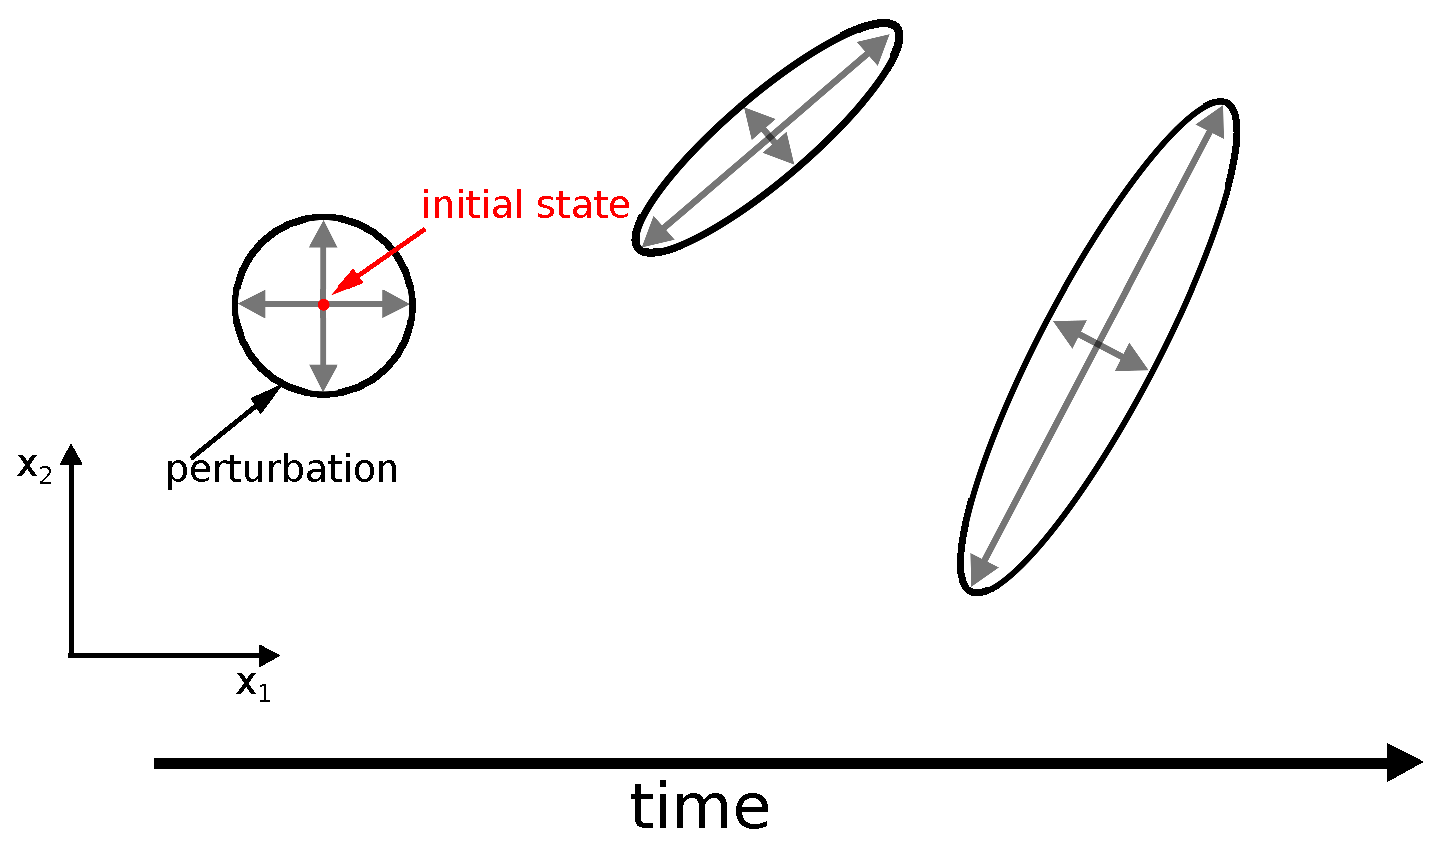
\includegraphics[width=0.8\textwidth]{graphics/phasespace_deform.eps}
    \caption[Deformation of Phase Space Volume]{Example of a deformation of a volume in a two-dimensional phase space: the red dot marks the deterministic initial state and the sphere the initial perturbation. The phase space volume of  the initially spherical perturbation is deformed with respect to the stability properties of the dynamical system \cite{kalnay2003atmospheric}.}
    \label{fig:phasespace}
\end{figure}
The deformation of the sphere is determined by its axes $a_{1}, \  ..., \ a_{n}$. The axes describe the separation rates of the trajectories, that started infinitesimally close. A parameter $\vec{\lambda} = (\lambda_{1},  ... ,\lambda_{m})$ is introduced so that any axis becomes the initial length scaled by $\lambda_{j}$ after a time $t$
\begin{equation}
    a_{i}(t) = a_{i}(0) e^{\lambda_{j}t} \quad ,
\end{equation}
resulting in a deformation of the volume of the sphere
\begin{equation}
    V(t) = V(0) \ e^{-\sum^{m}_{j=1} \lambda_{j}t} \quad .
\end{equation}
The coefficients $\lambda_{j}$  are called Lyapunov-exponents and their indices denote their relative magnitude:
\begin{equation}
  \forall  \lambda_{j}:\lambda_{j} \geq  \lambda_{j+1} \quad .
\end{equation}
Then the condition for a Hamiltonian system of the conservation of the initial volume of the sphere in phase space can be expressed as:
\begin{equation}
    \sum^{m}_{j=1}\lambda_{j} =0 \quad
\end{equation}
the condition for a stable system:
\begin{equation}
     \forall  \lambda_{j}:\lambda_{j} \leq 0
\end{equation}
and the condition for a chaotic system:
\begin{equation}
    \exists  \lambda_{j}:\lambda_{j} > 0 \quad .
\end{equation}
As those conditions imply, the volume contained in the sphere is conserved or can even converge to a point for a stable system. For a chaotic system at least $\lambda_{1}$ has to be greater than zero, so that trajectories in phase space diverge. In the textbook by \citeauthor{kalnay2003atmospheric} \cite{kalnay2003atmospheric} the meaning of the Lyapunov-exponents is summarized as the following: `[...]the Lyapunov-exponents describe the long-term average exponential rate of stretching or contraction in the attractor.'. The term attractor is used for the set of points that the trajectories pass multiple times.\\
For a stable system, reliable forecasts can be done at all times, where on the other hand, chaotic systems become unpredictable after a finite time. The Lyapunov-exponents and hence, the predictability of a system, can be calculated from theory or from experimental data \parencite{eckmann1986liapunov, vannitsem2017predictability, leutbecher2008ensemble}.



\subsection{Ensembles}

Since the beginning of the 1990s  ensemble prediction has become a widely-known approach to treat uncertainty in NWP and it is still considered state of the art and subject of current research with increasing popularity \cite{wilks2011statistical, bauer2015quiet, leutbecher2008ensemble, Shemyakin2018,palmer1993ensemble}. 
To estimate the effect of different values for the initial and boundary condition and model parametrizations  a so-called ensemble is created.
Each ensemble member represents a different simulation. It is a single trajectory in the phase space of the atmospheric system. For traditional ensembles independent runs for all members are performed and the statistical properties of the whole ensemble data set are evaluated \cite{leutbecher2008ensemble}.\\
There are three main types of ensembles:
\begin{enumerate}
\item {Multi-model ensemble: Each member uses a different NWP model  \cite{ebert}}
\item{Multi-physics ensemble: Each member uses different parametrizations or different settings of the model physics \cite{Houtekamer}}
\item{Traditional ensemble: Each member is obtained by perturbing one or more quantities in initial or boundary conditions, or in the model itself. If random number sampling is used, it is called Monte-Carlo forecast.}
\cite{du2007uncertainty, wilks2011statistical, leith1974theoretical}
\end{enumerate}
Figure \ref{fig:ecmwf_ensemble} shows an example of a traditional ensemble forecast and its components: ensemble forecasts contain several regular members and a control member, which is the deterministic scenario (the scenario considered most likely), with the same resolution as the other ensemble members. In most cases, the deterministic run is performed with a higher resolution, to get the best possible forecast. Unfortunately it would consume too much computational resources to run the whole ensemble on the highest possible resolution. Thus, a control member is computed additionally, to have a point of reference for the other ensemble members without the bias of different resolutions.\\
Depending on the type and source of uncertainty we want to investigate, we need to create an appropriate ensemble.\\
\begin{figure}[H]
    \centering
    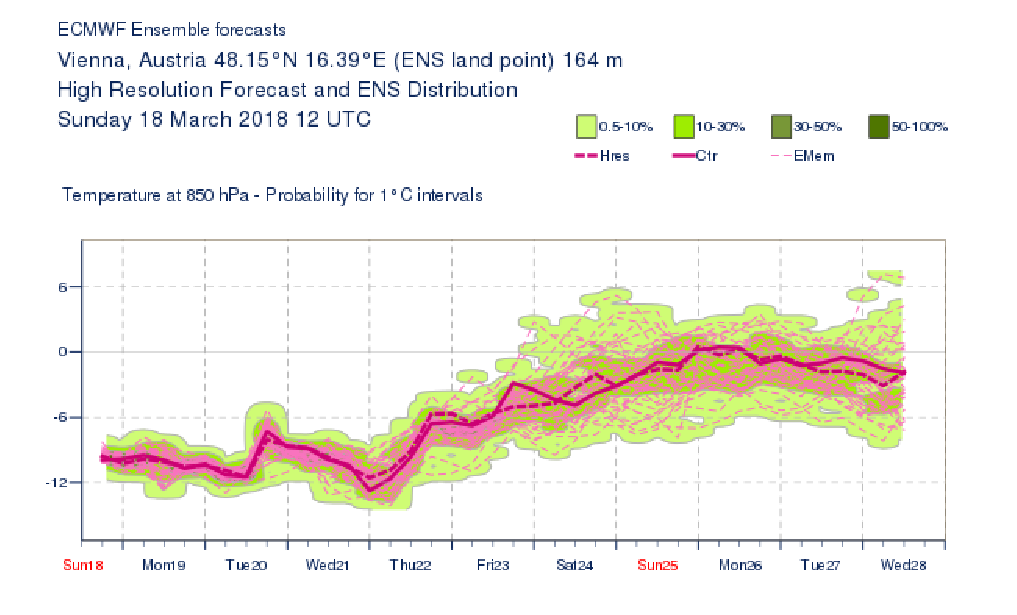
\includegraphics[width=0.8\textwidth]{graphics/ecwmfensemble_clip.eps}
    \caption[Example of Ensemble Forecast]{ECMWF ensemble: A temperature ensemble forecast of the ECMWF showing 50 regular members (`EMem'), one control member (`Ctr') and one high resolution run (`Hres'). The ensemble spread increases with time, revealing the chaotic dynamics of the atmosphere. The number of  ensemble members in a certain temperature interval can be related to the probability of a certain temperature. The image was created by the ECMWF (cannot be accessed by the public).}
    \label{fig:ecmwf_ensemble}
\end{figure}
In this study we focused on ensemble creation by stochastically perturbed parameters, a Monte-Carlo method, which is explained in greater detail in Subsection \ref{sec:Monte}.

\subsection{Uncertainty and Error}

The sources of error can be categorized into three groups: initial conditions, model error and, for limited area models (LAM), boundary conditions.
The initial conditions of the model equations have a very high level of uncertainty. Many of them are set by a best-guess gained from old model output combined with new measurements. But the number of measurement stations is usually small in comparison to the number of grid points in a model and also the measurement equipment has a limited accuracy. It is worth pointing out, that the problem is not only about the difference in number of grid points and measurement stations but also that the locations of grid points and measurement stations do not overlap. \\
The boundary conditions for limited area models are even more sensitive, because they are set to the output values obtained from a global model. Thus, errors can evolve and be amplified in the global model and are then passed on to the LAM, especially affecting the forecast quality on the edges of the domain.\\
A consequence of the limited resolution of the model is that many processes, that take place on a sub-grid scale, have to be parametrized.
Since every parametrization is an approximation, all parametrized physical processes contribute to the uncertainty in a model \cite{leutbecher2008ensemble}.
Even if a physical process is resolved explicitly, it contributes to model error, due to the model being discrete. In nature, on the other hand, most of the concerned processes evolve continuously on the model's scales. 
Another source of uncertainty is that for some quantities in the model, like aerosol concentration, only climatological data is used. The reason being, that  prognostic schemes require too much computational resources and/or there is a lack of up-to-date data. \\
A problem specific to NWP models is the orographic mismatch. Especially in mountainous regions not all topographic structures can be resolved. This can cause a large discrepancy between reality and model.\\

\subsection{Ensemble Creation by Monte-Carlo Methods}
\label{sec:Monte}
In a stochastic ensemble, each member represents a different possible value of a certain quantity. How the values differ for the members is determined by a random sampling regime. Ensemble members are created by perturbing a deterministic value, that we will call the unperturbed value from now on. But it is important to acknowledge that the unperturbed value shall never be seen as the `real' value of a variable, but the most likely value. A value being categorized as most likely can be based on climatological data, knowledge of the underlying physics or current measurement data. Because of limited accuracy of measurement equipment and the spatial resolution, it is inherently impossible to determine a `real' value of a variable in an atmospheric system. Only a certain range for the values can be determined. \\
We distinguish the different perturbation schemes by the perturbed quantity:
\begin{enumerate}
    \item {Perturbing the initial value of a variable}
    \item {Perturbing the tendency of a variable (SPPT)}
    \item {Perturbing constant parameters in a parametrization (SPP)}
\end{enumerate}
The SPPT and the SPP perturbation schemes are used to take model error into account. Perturbation of the initial values, on the other hand,  incorporates the errors contributed by the set-up of initial and/or boundary conditions.\\
The different schemes are briefly outlined in the following. 

\subsubsection{Perturbation of initial conditions }
The simple random perturbation of initial conditions is the most basic perturbation scheme.
Let $e_{j}$ be the time integration of the model equations (`prognostic variable')
\begin{equation}
    \frac{\partial e_{j}}{\partial t} = A(e_{j},t) + P(e_{j},c_{0},..., c_{N}) \quad ,
    \label{eq:icpert1}
\end{equation}
where $A$ are the non-parametrized and $P$ are the parametrized contributions, which depend on $e_{j}$, the time $t$ and $N$ constant parameters $c_{0},..., c_{N}$.\\
Now only the initial conditions are perturbed
\begin{equation}
    e_{j}(t=0) \equiv e_{j,0}+ \delta e_{j}(t=0) \quad ,
    \label{eq:icpert2}
\end{equation}
where $ e_{j,0}$ is the deterministic value at $t=0$ and $\delta e_{j}$ is the  perturbation.
From investigation of  Equation \eqref{eq:icpert1} and \eqref{eq:icpert2} it is obvious that the difference in the evolution of different ensemble members has its origin solely in the perturbation of initial conditions. The simplest way to set-up the perturbation is to only perform random sampling. But today more sophisticated techniques, like the use of Lyapunov-exponents, are more common than a plain Monte-Carlo approach \cite{0034-4885-63-2-201, buizza1999stochastic}.

\subsubsection{Stochastically Perturbed Parametrized Tendencies (SPPT)}
In the model equations the tendencies of all model variables are calculated at each time step and used for the integration. The tendency of a variable is defined as its change in one time step. It is the sum of the change of the variable calculated from the Primitive Equations $A(e_{j},t)$ and the change contributed by parametrized processes $P(e_{j},c_{0},..., c_{\mathrm{N}})$. Thus, $P(e_{j},c_{0},..., c_{\mathrm{N}})$ is called  parametrized tendency hereafter.
We start as before, but now the parametrized tendency $P$ is perturbed and denoted by $P^{\prime}$
\begin{equation}
    \frac{\partial e_{j}}{\partial t} = A(e_{j},t) + P^{\prime}(e_{j},c_{0},..., c_{\mathrm{N}}) \quad .
    \label{eq:sppt}
\end{equation}
For each grid point the perturbed parametrized tendency is defined as
\begin{equation}
   P^{\prime} \equiv r_{j}(\lambda_{\mathrm{lon}}, \phi, t) P \quad ,
\end{equation}
where $ r_{j}$ is a random number. It is taken from a spatially and temporally correlated pattern consisting of randomly sampled numbers, chosen from a suitable distribution \parencite{buizza1999stochastic}. Regarding Equation \eqref{eq:sppt}, it is noteworthy that only errors contributed by parametrizations are considered.


\subsubsection{Stochastically Perturbed Parameters (SPP)}
We start as before, but now the constant parameters $c_{0},..., c_{\mathrm{N}}$ in the parametrized tendency $P$ are perturbed. Therefore the resulting parametrized tendencies are denoted by $P^{\prime \prime}$ 
\begin{equation}
    \frac{\partial e_{j}}{\partial t} = A(e_{j},t) + P^{\prime \prime}(e_{j},c_{0}r_{0},..., c_{\mathrm{N}}r_{\mathrm{N}}) \quad .
\end{equation}

For each grid point the perturbed parametrization is defined as
\begin{equation}
   P^{\prime \prime} \equiv  P^{\prime \prime }(e_{j}, c_{0} r_{0}(\lambda_{\mathrm{lon}}, \phi, t), ..., c_{\mathrm{N}} r_{\mathrm{N}}(\lambda_{\mathrm{lon}}, \phi, t)) \quad ,
\end{equation}
where again, $ r_{j}$ is a random number, taken from a spatially and temporally correlated
pattern consisting of randomly sampled numbers. In this regime the uncertainties can be directly related to single physical parameters \parencite{ollinaho2017towards}.\\ \\

The choice of scheme depends on what we want to examine and how the sources of error should be weighted.

For example, if we want to investigate the effect of the variation of initial conditions due to limited accuracy in measurements and hence, in data assimilation, then the initial value of the variable needs to be perturbed.
To examine the effects of uncertainty due to model error, introduced by spatial and time discretization, the tendencies of the variables should be perturbed as well. There are many parametrized processes contributing to the tendencies, so perturbing the tendencies can be an effective way to increase model spread based on acknowledging the effect of uncertainties in different parametrizations.\\

If we obtained a parametrization e.g. by fitting data, then, to analyse the impact of the uncertainty of the coefficients, the constant parameters can be perturbed.

To decide which variables, parameters or tendencies should be perturbed, one has to identify those, which have the highest level of uncertainty and which are most influential to the model output. Moreover, one must consider what is computationally affordable and stable.\\



%Rayleigh and Mei scatteing theory mit plots
\section{Visibility}
\label{sec:visib}
Since this study focuses on forecasting visibility, the most important definitions, mathematical derivations and physical processes related to it, are presented in this Section.
\subsection{Definitions}
The World Meteorological Organization (WMO) sets all standards and definitions for meteorological measurements, forecasts and procedures, including visibility observation. It  provides three important definitions in the context of visibility \cite{WMO}:
\begin{itemize}
    \item {The \textbf{meteorological optical range} is the length of path in the atmosphere required to reduce the luminous flux in a collimated beam from an incandescent lamp, at a colour temperature of 2700 K, to 5\% of its original value, the luminous flux being evaluated by means of the photometric luminosity function of the International Commission on Illumination (CIE). }
    \item{ \textbf{Visibility, meteorological visibility (by day) and meteorological visibility at night} are defined as the greatest distance at which a black object of suitable dimensions (located on the ground) can be seen and recognized when observed against the horizon sky during daylight or could be seen and recognized during the night if the general illumination were raised to the normal daylight level.}
    \item { \textbf{Visual range (meteorological)}: Distance at which the contrast of a given object with respect to its background is just equal to the contrast threshold of an observer.}
\end{itemize}


%This thesis focuses on forecasting visibility, for which \citeauthor{clark2008prediction} \cite{clark2008prediction} state the following:
%\begin{quote}
%`Visibility represents the shortest horizontal distance %visible, considering all directions'
%\end{quote}

%The `visible distance' means the distance, for which an %object is still visible for a human observer. 
%To be able to observe an object, it has to have a contrast $C$, with respect to its background, that lies above a contrast threshold value $\varepsilon$. 
Regarding their definitions, the meteorological visibility and the visual range are closely related. The meteorological visibility is mostly relevant for human observers, denoting always the lowest value considering all horizontal directions. Although the WMO sets the meteorological optical range as the measurement standard, the meteorological visibility is the recommended approximation for human observers, since it can be understood intuitively. Because most visibility measurements are still performed by human observers, meteorological visibility is the measure for visibility in praxis.\\ \\
\citeauthor{koschmeider1924theorie} was the first one to derive a mathematical expression for visibility, using the visual range \cite{koschmeider1924theorie}.\\
Also in most models the visual range is used, because it provides a more thorough definition than the meteorological visibility and is therefore easier to be implemented, but still relates to the observed visibility. The mathematical derivation is briefly outlined in the following section according to \citeauthor{price2007advanced} \cite{price2007advanced}, who refers to the works of \citeauthor{koschmeider1924theorie} \cite{koschmeider1924theorie}.

\subsection{Mathematical Derivation of Visibility and Visual Range}

Let the contrast $C$ be defined as 
\begin{equation}
    C=\frac{ B_{b} - B_{a} }{B_{b}} \quad ,
\end{equation}
where $B_{b}$ denotes the brightness of the background and $B_{a}$ the brightness of the object,
and let the change of the brightness on an infinitesimal line segment along a horizontal line $x$ be
\begin{equation}
    \frac{dB}{dx}=- \beta_{\mathrm{tot}}B + B_{s} \quad ,
    \label{eq:fracB}
\end{equation}
where $ \beta_{\mathrm{tot}}$ denotes the total atmospheric extinction coefficient and  $B_{s}$ denotes the light that is being scattered in the line. Equation \eqref{eq:fracB} can also be applied to $B_{b}$.
Since the brightness of the background is independent of the distance, the following condition is satisfied:
\begin{equation}
    \frac{dB_{b}}{dx}=0 \quad .
\end{equation}
Then, the change of contrast along an infinitesimal line segment can be written as
\begin{equation}
    \frac{d C }{dx} = -\frac{1}{B_{b}} \frac{B_{a}} {dx}  \quad .
    \label{eq:contrastfrac}
\end{equation}
Evaluating Equation \eqref{eq:fracB} for the brightness of the background we gain the expression
\begin{equation}
    \beta_{\mathrm{tot}}B_{b}= B_{s} \quad .
    \label{eq:background}
\end{equation}
When plugging \eqref{eq:background} into Equation \eqref{eq:fracB} and evaluating Equation \eqref{eq:contrastfrac} we get
\begin{equation}
    \frac{d C}{d x} = - \beta_{\mathrm{tot}} C
    \label{eq:CDE} \quad .
\end{equation}
As Equation \eqref{eq:CDE} implies, we can use an exponential ansatz and get the necessary boundary conditions by investigation of the case of a perfectly black object in front of a white background. In the considered scenario, the contrast of the object at the point of the observer has to be 100\%, because all light is absorbed. Also, the contrast should go to 0 for the object being infinitely far away. Hence, the following equations need to be satisfied:

\begin{eqnarray}
     C(x=0)&=&1\\
     \lim_{x \to \infty} C(x)&=&0 
\end{eqnarray}

With these boundary conditions the coefficients of the contrast are derived as an exponential function of the distance between the observer and the object
\begin{equation}
    C(x)=\exp (-\beta_{\mathrm{tot}}x) \quad .
\end{equation}
From this we can derive the maximum distance for which the contrast is still above the contrast threshold value. This distance is called the `visual range'. Since the atmospheric extinction can vary for different directions, the visual range can vary too. The minimum of the visual range, considering all directions, is approximately the visibility $vis$. For reasons of computational simplicity, we only use the atmospheric extinction of the point where the visibility is forecast. Hence, the visual range and the visibility are equivalent in this study and defined by 
\begin{equation}
    vis = -\frac{ \ln ( \varepsilon)} { \beta_{\mathrm{tot}}}    \quad .
    \label{visibility}
\end{equation}
The contrast threshold $\varepsilon$ should be chosen under the consideration of the purpose and usage of the visibility data.
Most authors suggest to set the contrast threshold to $2 \% $ (e.g. \citeauthor{ballard1992diagnosis} \cite{ballard1992diagnosis}) while other consider  $5 \% $ to be more accurate  (e.g. \citeauthor{claxton2008using} \cite{claxton2008using}). 
The differing values are due to the fact that the contrast is chosen with respect to what our eyes are gauged to. But as we experience in our everyday life, this can vary for different people, shapes and colours \parencite{koschmeider1924theorie}. As this implies, the constant setting of $\varepsilon$ is an approximation for the sake of simplicity. 






\subsection{Atmospheric Scattering}


Mie and Rayleigh scattering are special cases of scattering of electromagnetic waves on a homogeneous sphere \cite{hulst1957light}. Both scattering regimes together are sufficient to describe the most important scattering processes in the atmosphere.  Mie scattering, for example, is responsible for visibility reduction due to fog and for clouds being perceived as white. To observe the effects of Rayleigh scattering, one must simply look at the  blue colour of the clear sky \cite{wallace2006atmospheric}. 
Generally, if we aim to describe a radiative process with one of the two theories, we need to verify first, if it is suitable for the process' size range. To be able to do so, a size parameter $\alpha$ is introduced. It depends on the radius of the sphere $r$ and the wavelength of the incoming light $\lambda$ and is defined as
\begin{equation}
    \alpha = \frac{ 2 \pi r }{\lambda} \quad .
\end{equation}
For Rayleigh scattering the condition
\begin{equation}
    \alpha \ll 1
    \label{eq:Rayleighcon}
\end{equation} must hold. In other words, the radius of the object must be much smaller than the wavelength of the incoming radiation.
In the Earth's atmosphere Rayleigh scattering is mostly contributed by scattering on air molecules and much less variable in time and space than the contribution by Mie scattering. \\
Another difference between the to regimes is that Rayleigh scattering strongly favours shorter wavelengths and therefore in the visible spectrum the colour blue. Mie scattering on the other hand, has a very weak dependence on the wavelength \cite{raith2001erde}. As a result we see most Mie-scattered sunlight as white, because it contains all wavelengths of the sun's spectrum.
The Mie scattering regime can be applied for all cases where 
\begin{equation}
     0.1<\alpha<50
     \label{eq:Miecondition}
\end{equation}
holds. \\
For visible light, which has a wavelength from approximately 390nm to 700nm,  the condition is satisfied for scattering on vapour, hydrometeors and aerosols \parencite{wallace2006atmospheric, chandrasekar2010basics}.
Due to the dominating physical process being Mie scattering  \parencite{price2007advanced}, there is a strong dependency of the total atmospheric extinction coefficient on the specific humidity, precipitation, cloud water in liquid and ice form and aerosols. The relations can be derived by characterizing the hydrometeors and aerosols in the air as a suspension of perfect spheres with different refractive indices and radii in a gas \cite{lang2010interaction}. Figure \ref{fig:red-on-raindrop} illustrates an example of atmospheric scattering: visible red light on a water drop. The plot shows a peak for forward scattering, typical for the angular intensity distribution of Mie scattering.
%The extinction efficiency for the different spheres is calculated and used to derive mass
\begin{figure}
    \centering
    \begin{subfigure}{0.45\textwidth}
 %       \captionsetup{width=\textwidth}
        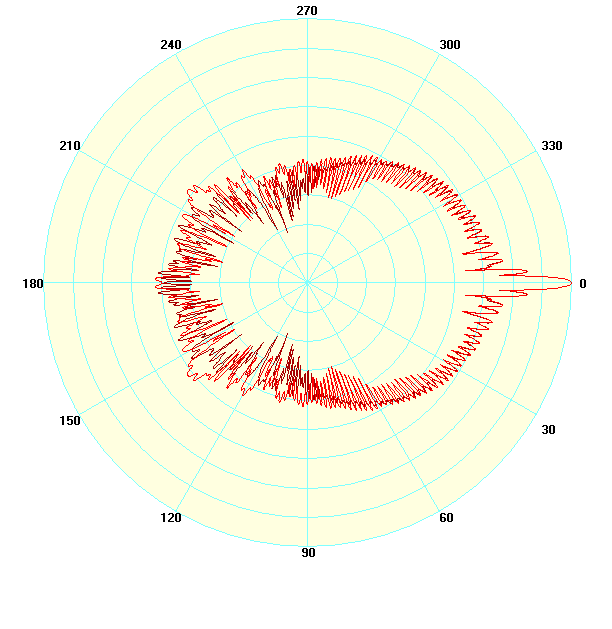
\includegraphics[width=\textwidth]{graphics/650nmonWaterEdited.png}
        \caption[Scattering on a Rain Drop]{Scattering of visible red light ($\lambda$=650nm) on a water drop.\\ Used parameters: particle radius: 1.0e-05 m; refractive index: 1.33257 + i1.67e-08; scale: logarithmic, value at outer circle: 2.18e+07, value at inner circle: 2.18e-02.\label{fig:red-on-raindrop}  }    
    \end{subfigure}
    \hspace{1cm}
    \begin{subfigure}{0.45\textwidth}
        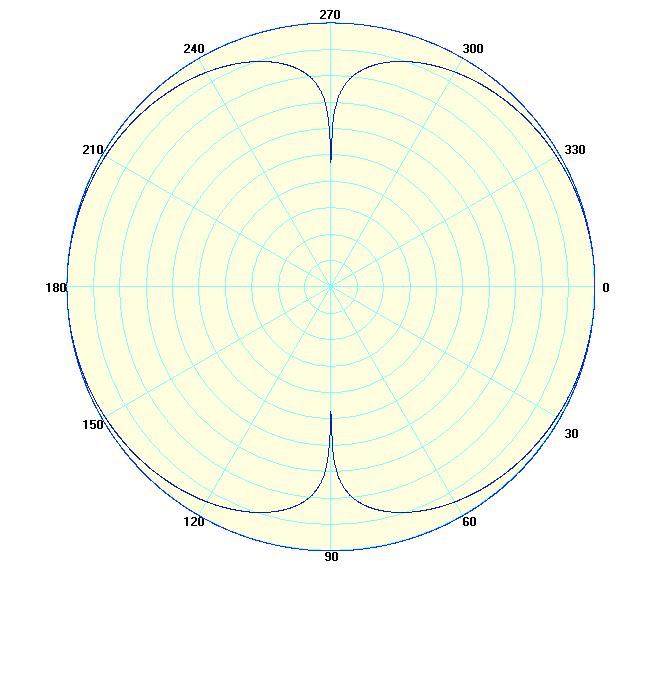
\includegraphics[width=\textwidth]{graphics/Rayleighscatter.png}
        \caption[Scattering on a Rain Drop]{Scattering of visible blue light ($\lambda$=400nm) on an oxygen molecule.\\ Used parameters: particle radius: 1.52e-10 m; refractive index: 1.000152; scale: logarithmic, value at outer circle: 2.5e-24, value at inner circle: 2.18e-34. \label{fig:blue-on-oxygen}  }
    \end{subfigure}
    \caption[Scatter Plots of Mie and Rayleigh scattering]{Scatter plot of Mie and Rayleigh scattering: Intensity versus scattering angel. \\Created by the use of \citetitle{laven2011mieplot} }
\end{figure}
%But because these quantities all interact with other model variables in a non-linear way, implicitly temperature, pressure and many other variables have great impact on the visibility as well. \\





The scattering characteristics of a material are described by their extinction, scattering and absorption coefficients. In the course of predicting  visibility, we are only interested in the extinction coefficient to be able to quantify the total reduction the light's intensity \cite{horvath1981atmospheric}.
The extinction coefficient $ Q_{ext}$ is the dimensionless equivalent of the extinction cross section $C_{ext}$ and defined as
\begin{equation}
    Q_{ext}=\frac{C_{ext}}{G} \quad ,
\end{equation}
where $G$ is the geometric factor that is set to $\pi r^{2}$ for spherical particles, because of their circular cross section.

The extinction cross section is a measure for the total difference in radiant flux through a defined surface $S$. The two compared cases are, when a particle is present at a location and when it is not. The extinction cross section is defined as 
\begin{equation}
C_{ext}=\frac{1}{E^{i}} \int_{4\pi R^{2}} (E^{i}-E)dS \quad ,
\label{eq:extcoef1}
\end{equation}
where $E^{i}$ denotes the electric field vector when there is no particle at the location, and $E$ when a particle is present. The boundary surface $S$ is set to the surface of a sphere because we are interested in the case of scattering on spherically approximated particles.
For aerosol scattering the electric field vectors can be obtained by the use of Mie scattering theory. The theory was first developed by Gustav    \citeauthor{mie1908beitrage} \cite{mie1908beitrage} and is derived by applying boundary and continuity conditions for light approaching a sphere to Maxwell's equations.\\
The resulting wave functions are in form of power series composed of Bessel functions and Legendre polynomials \parencite{kerker2016scattering}.
When inserting these in Equation \eqref{eq:extcoef1} we derive the following mathematical expression for the extinction cross section:
\begin{equation}
C_{ext}=-\frac{2 \pi }{k^{2}_{0}} \Re \left( \sum_{n=1}^{ \infty} (2n +1) (a^{s}_{n} + b^{s}_{n}) \right) \quad ,
\label{eq:extcoef2}
\end{equation}
where $k_{0}$ is the wave number in vacuum and $a^{s}_{n}$ and  $b^{s}_{n}$ are the Mie coefficients. Those are derived as part of the solution when solving the scalar wave equation. The Mie coefficients are composed of Riccati-Bessel functions and include a dependency on the refractive index. The entire detailed derivation is presented in several textbooks e.g. \cite{zdunkowski2007radiation}, \cite{hulst1957light}.
Regarding Equation \eqref{eq:extcoef2}, we see that only an approximation of $C_{ext}$ can be calculated numerically and the accuracy depends mainly on the number of terms computed. Many different algorithms for the computations were developed and \citeauthor{wriedt2009light} \cite{wriedt2009light} provides a good overview with special focus on the application on aerosols. \\
As mentioned, the second most relevant scattering process in the atmosphere is Rayleigh scattering. Regarding the criterion presented in Equation \eqref{eq:Rayleighcon}, it is obvious that Rayleigh scattering takes place, if the size of the particle is much smaller than the incoming wavelength. It is a result of the polarizability of the gas molecules: the incoming electromagnetic wave excites the molecules, so that each molecule acts as Hertzian dipole. Figure \ref{fig:blue-on-oxygen} illustrates an example of visible blue light being scattered on an oxygen molecule and shows the characteristic angular intensity distribution of a Hertzian dipole. It radiates  with the same wavelength as the incoming light. This is also true for Mie scattering.
Such processes, without a shift between the wavelength of the scattered light and the incident light, are called elastic, because the change in energy of the photons is negligibly small.

\chapter{Model}
\label{sec:model}
The model we used for this study, is called `Application of Research to Operations at Mesoscale' (AROME) and was developed by the ALADIN consortium  \cite{aladinhp}. At the `Zentralanstalt für Meteorologie und Geophysik' (ZAMG), the model has been operational since 2014, which means that it is not only used for research, but also for forecasts on a daily basis.  If not mentioned otherwise, all settings remained the same as for the operational configuration of the model at ZAMG.\\
As the name implies, AROME is a limited area model, written in Fortran. The version operationally used at ZAMG (C40T1) has a horizontal resolution of 2.5km on a 432-by-600 grid and 90 vertical layers. The highest layer is at a pressure level of 10hPa, which is the equivalent of approximately 25km. One time step is set to  60 seconds and the geographical model domain of central Europe is shown in several graphics in the following (e.g. Figure \ref{fig:stations} , \ref{fig:example-pert} ). It is a convection permitting and non-hydrostatic model \cite{gmd-2017-103}. Convection permitting means that ascending and descending convective currents are resolved, opposed to the strategy of simply parametrizing their effects, commonly done in global models with a lower resolution.\\
Since AROME is a LAM, it has to be nested in a model with a larger domain, to set its boundary values. At ZAMG the used model is the global European `Integrated Forecast System' (IFS), version C41R2, developed by the European Centre for Medium-Range Weather Forecasts (ECMWF) \cite{IFS}. The IFS model is operationally run with a 51 member ensemble at the ECMWF. ZAMG uses a subset of 16 members and the control member of the ECMWF-ensemble. \\
AROME was forked from the original ALADIN (Aire Limitée Adaptation Dynamique Développement International) model, which was developed by Météo-France. \\
Most parts of the code are contained in the common code package IAAA (IFS, ALADIN, AROME, ARPEGE) where AROME is a canonical configuration of the package \parencite{gmd-2017-103} and uses the so-called `MESO-NH' physics package \parencite{lafore1998p}.\\
For its dynamical core AROME uses a semi-implicit semi-Lagrangian scheme \parencite{gmd-2017-103,seity2011arome}. The Lagrangian and the Eulerian schemes are different methods for treating flow fields in continuum mechanics. A Lagrangian scheme describes a system by the movements of the parcels of the fluid. The counter-model of that, the Eulerian scheme, uses the change rates at specific locations to capture the dynamics of the field. In a semi-Lagrangian scheme an Eulerian grid is used and at each time step the trajectories that brought the parcels of the fluid to their current locations are calculated \cite{durran2010numerical}. The main reason why semi-Lagrangian schemes very common in NWP models is, because when combined with semi-implicit integration, they remain stable even for long time steps \cite{vincent}. 


\section{Spatial Discretization}
\begin{wrapfigure}{l}{0.4\textwidth}
    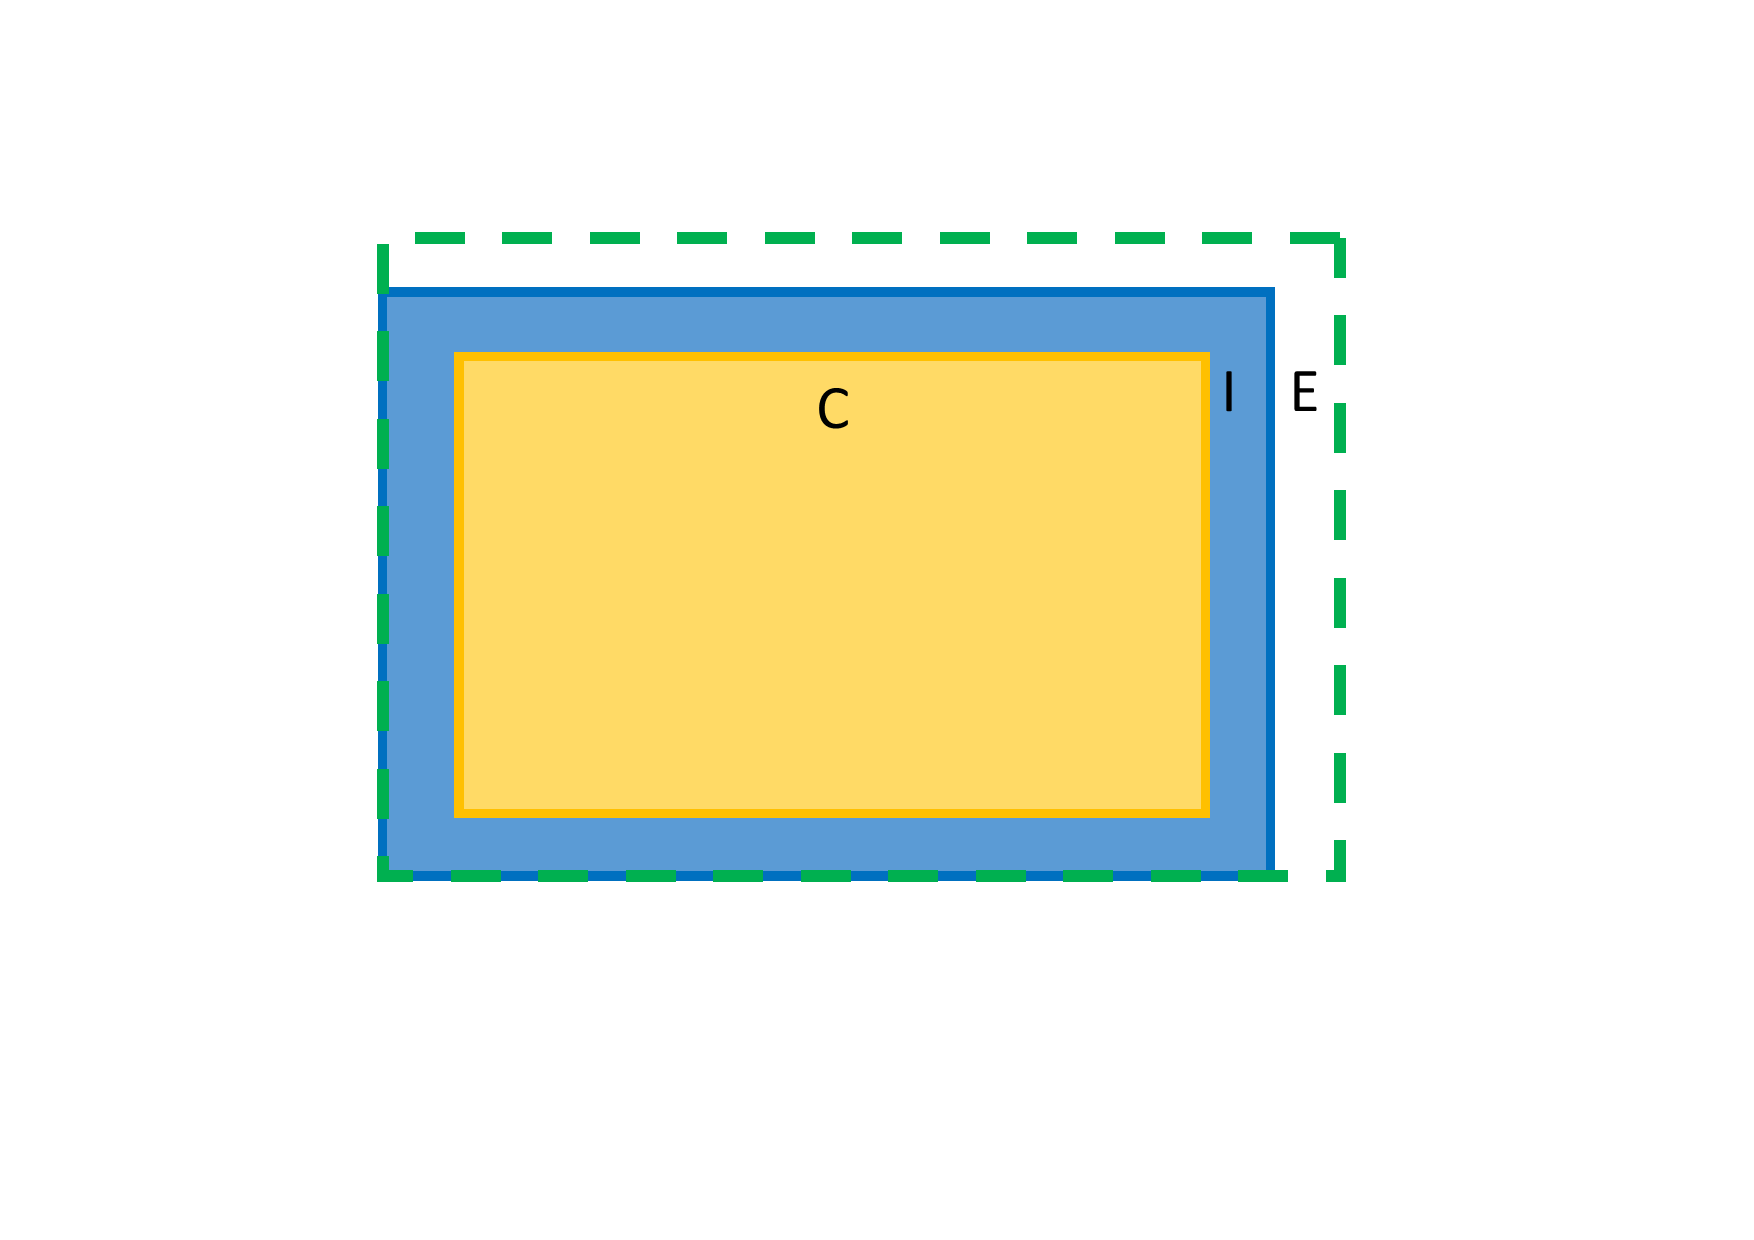
\includegraphics[trim={5cm 5cm  5cm  4cm },clip,
     width=0.9\linewidth] {graphics/Zones.png}
    \caption[Zones in AROME's Computational Domain]{Different Zones in AROME model domain: C - Central Zone, I - Intermediate Zone, E - Extension Zone \parencite{gmd-2017-103}}
    \label{fig:zones}
\end{wrapfigure}The AROME Model mainly uses spectral representations of the fields, with the exception of the grid point representation of humidity. Each time, fields of different types need to interact, a Fast Fourier Transformation (FFT) is performed. \\
The spectral horizontal discretization is a bi-Fourier spectral representation with elliptical truncation on a conical Lambert-projection, as illustrated in Figure \ref{fig:lambert}. The vertical discretization uses finite differences and finite elements \parencite{gmd-2017-103, meteofrance}.  
\\
Due to the bi-Fourier spectral representation, different zones (as shown in Figure \ref{fig:zones}) had to be introduced in the model.
The outermost zone E is called extension zone and is the actual computational domain of the spectral method. 
Because of the periodic nature of the Fourier Series the computational domain describes a torus. Consequently, it can never be congruent with the geographical LAM domain. To resolve this issue, the corresponding geographical domain is a cut-out of the extension zone to avoid physically nonsensical periodic values at the edges of the domain.
In the Intermediate Zone I the boundary conditions from the global model get sourced in.
Only in the Central Zone C can the physics and dynamics evolve completely freely. This zone can be seen as the equivalent of the geographical domain \cite{gmd-2017-103}.\\
The vertical coordinate is a hybrid pressure terrain-following coordinate. It is preferred over a simple pressure coordinate, because as illustrated in Figure \ref{fig:coordinates}, geographical barriers like mountains are considered.
\begin{figure}[H]
    \centering
    \begin{subfigure}{0.45\textwidth}
    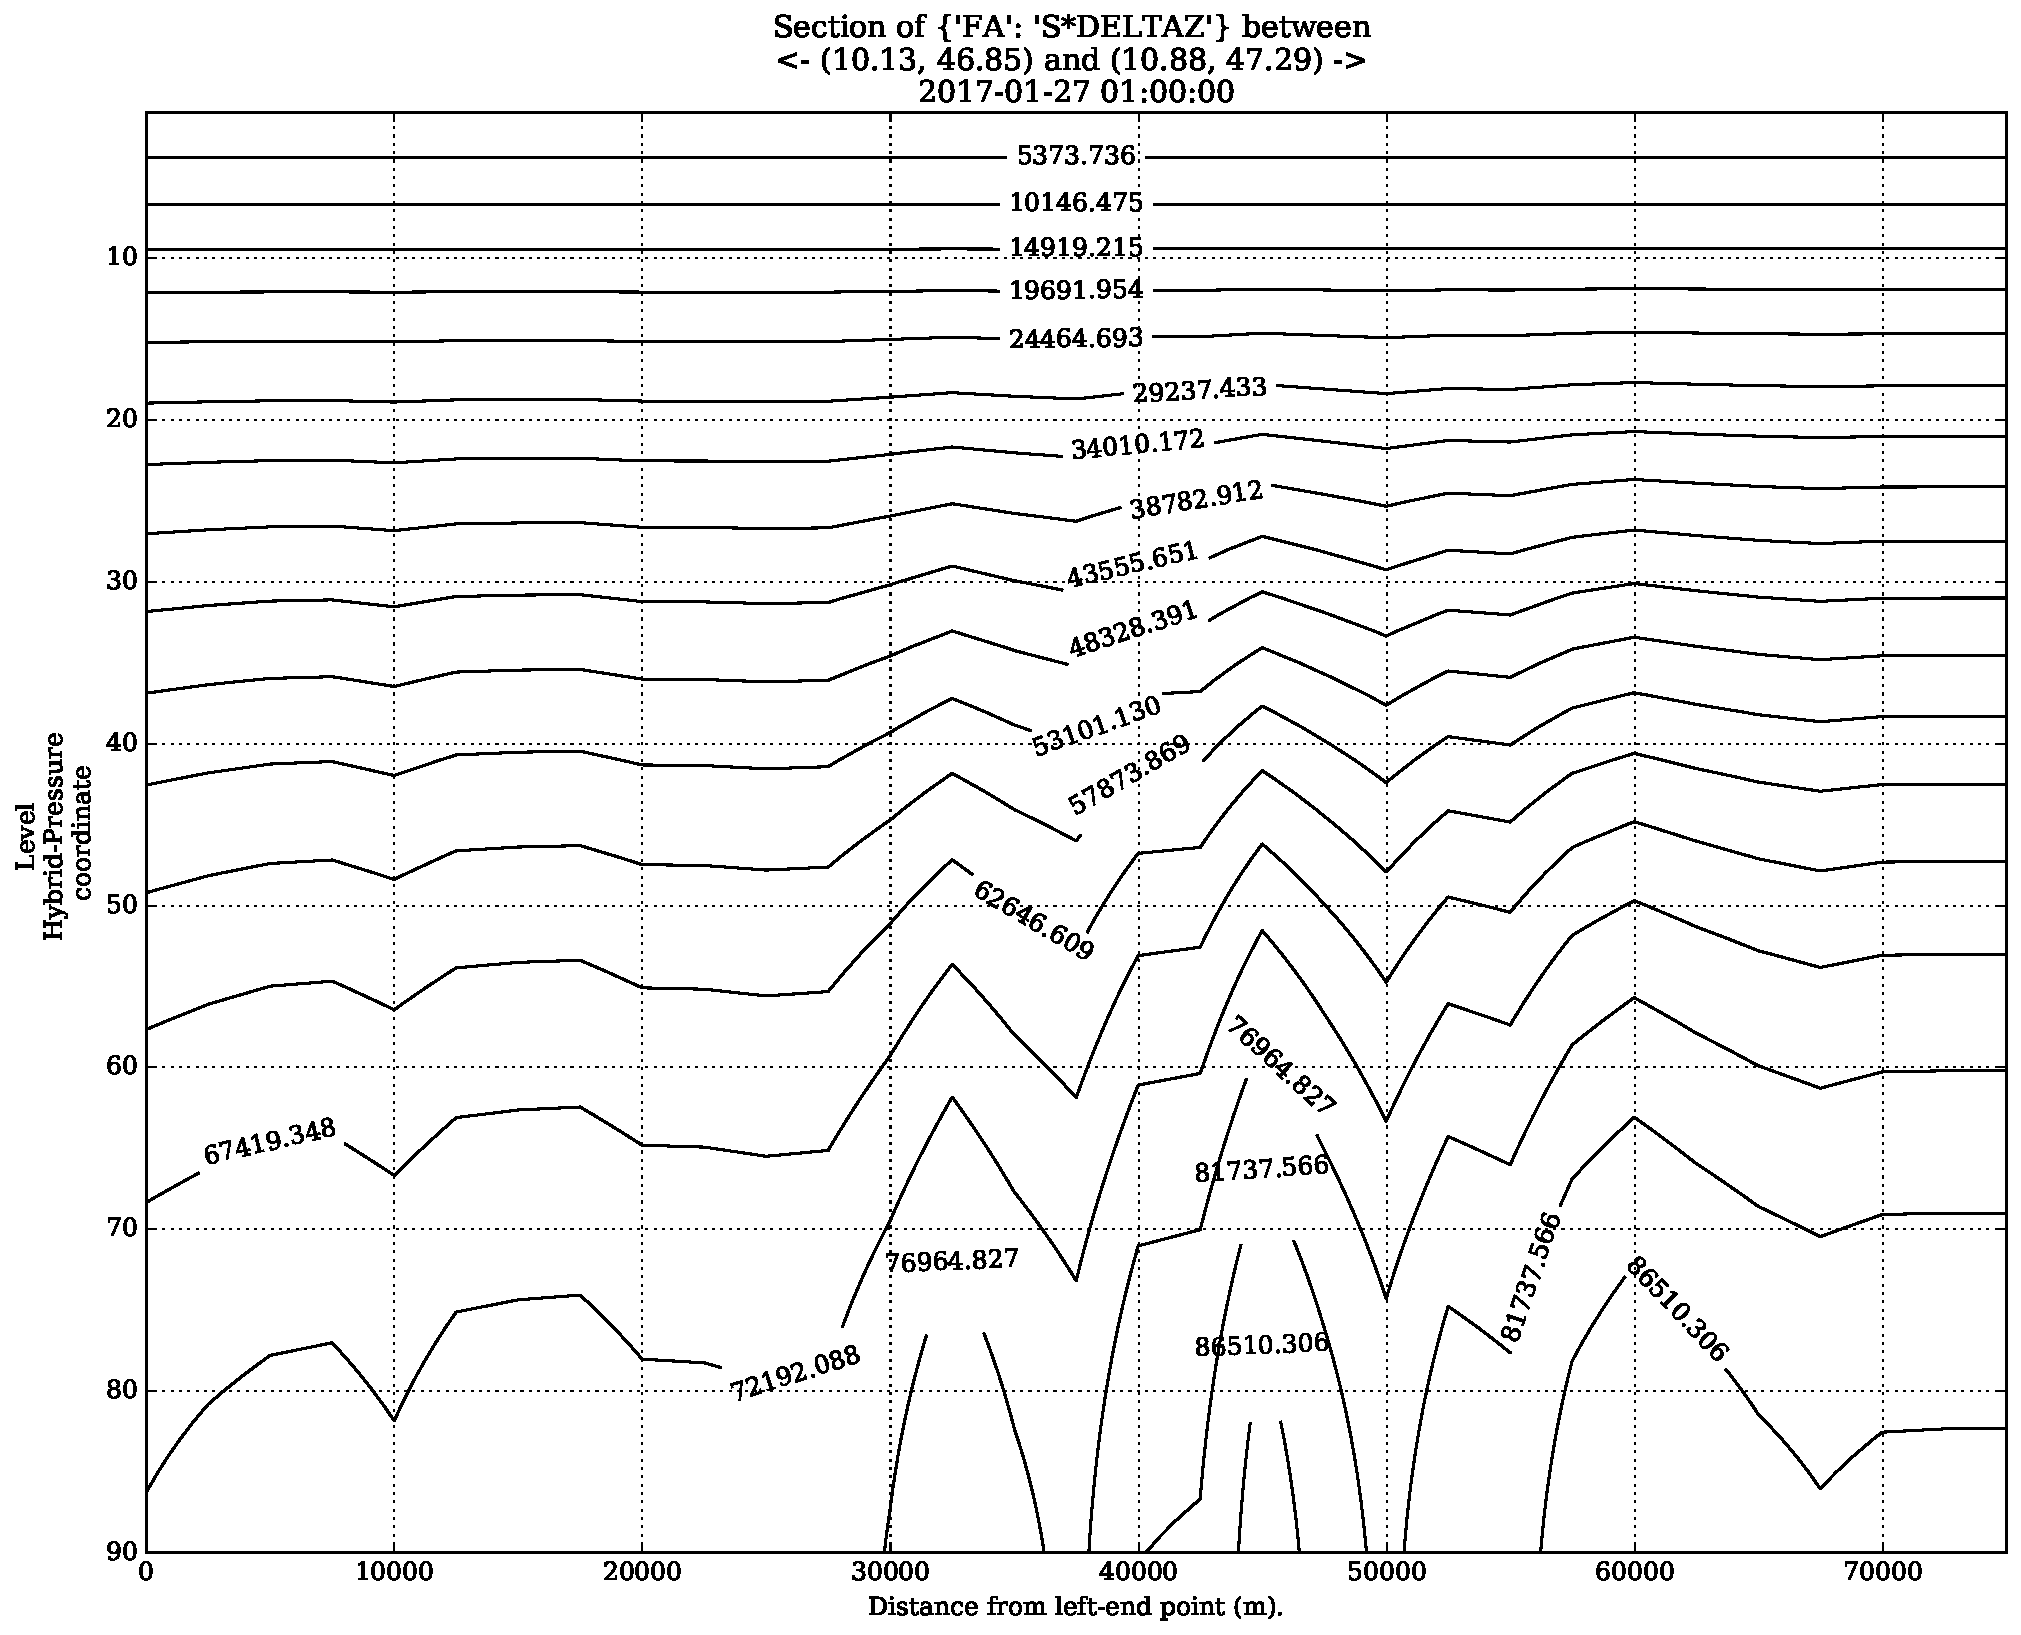
\includegraphics[trim={0cm 0cm  0cm  1.8cm },clip,width=\textwidth]{graphics/coordinates/PvsHybrid.pdf}
    \caption{\footnotesize{Hybrid Pressure-Terrain-following coordinates: layer number on Y-axis}}
    \label{fig:PvsHybrid}
    \end{subfigure}
    \hspace{1cm}
    \begin{subfigure}{0.45\textwidth}
    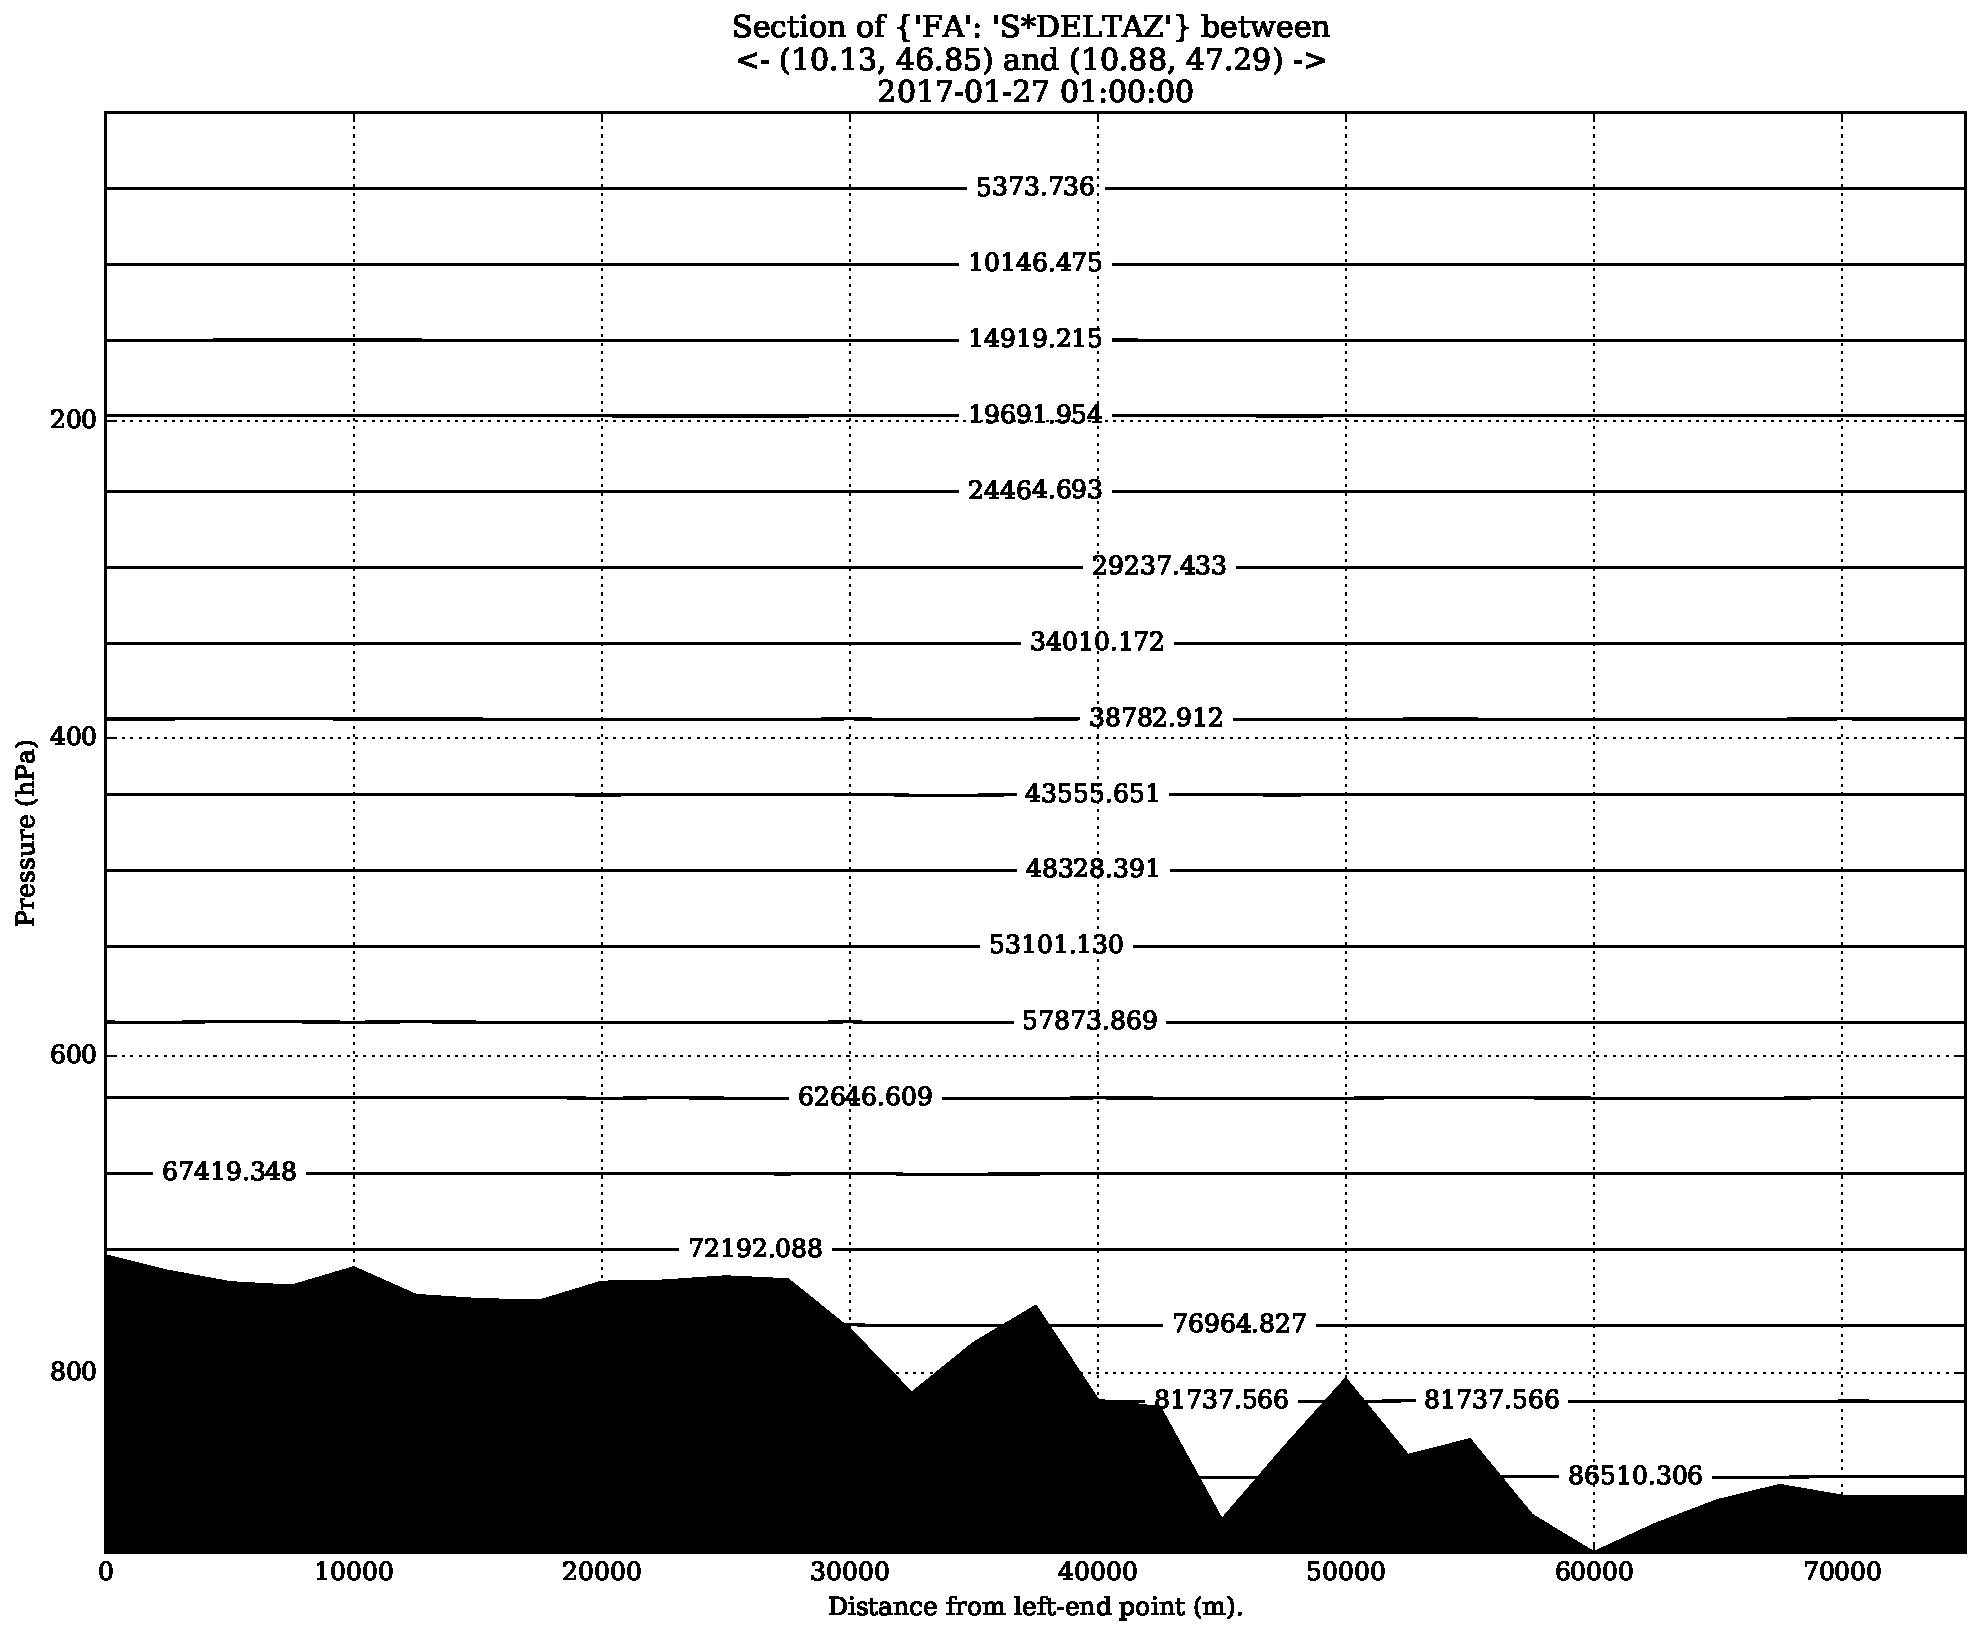
\includegraphics[trim={0cm 0cm  0cm  1.8cm },clip,width=\textwidth]{graphics/coordinates/PvsPressure.pdf}
    \caption{\footnotesize{Pressure coordinates: pressure [hPa] on Y-axis}}
    \label{fig:PvsP}
    \end{subfigure}
    \vspace{1cm}
    \begin{subfigure}{0.45\textwidth}
    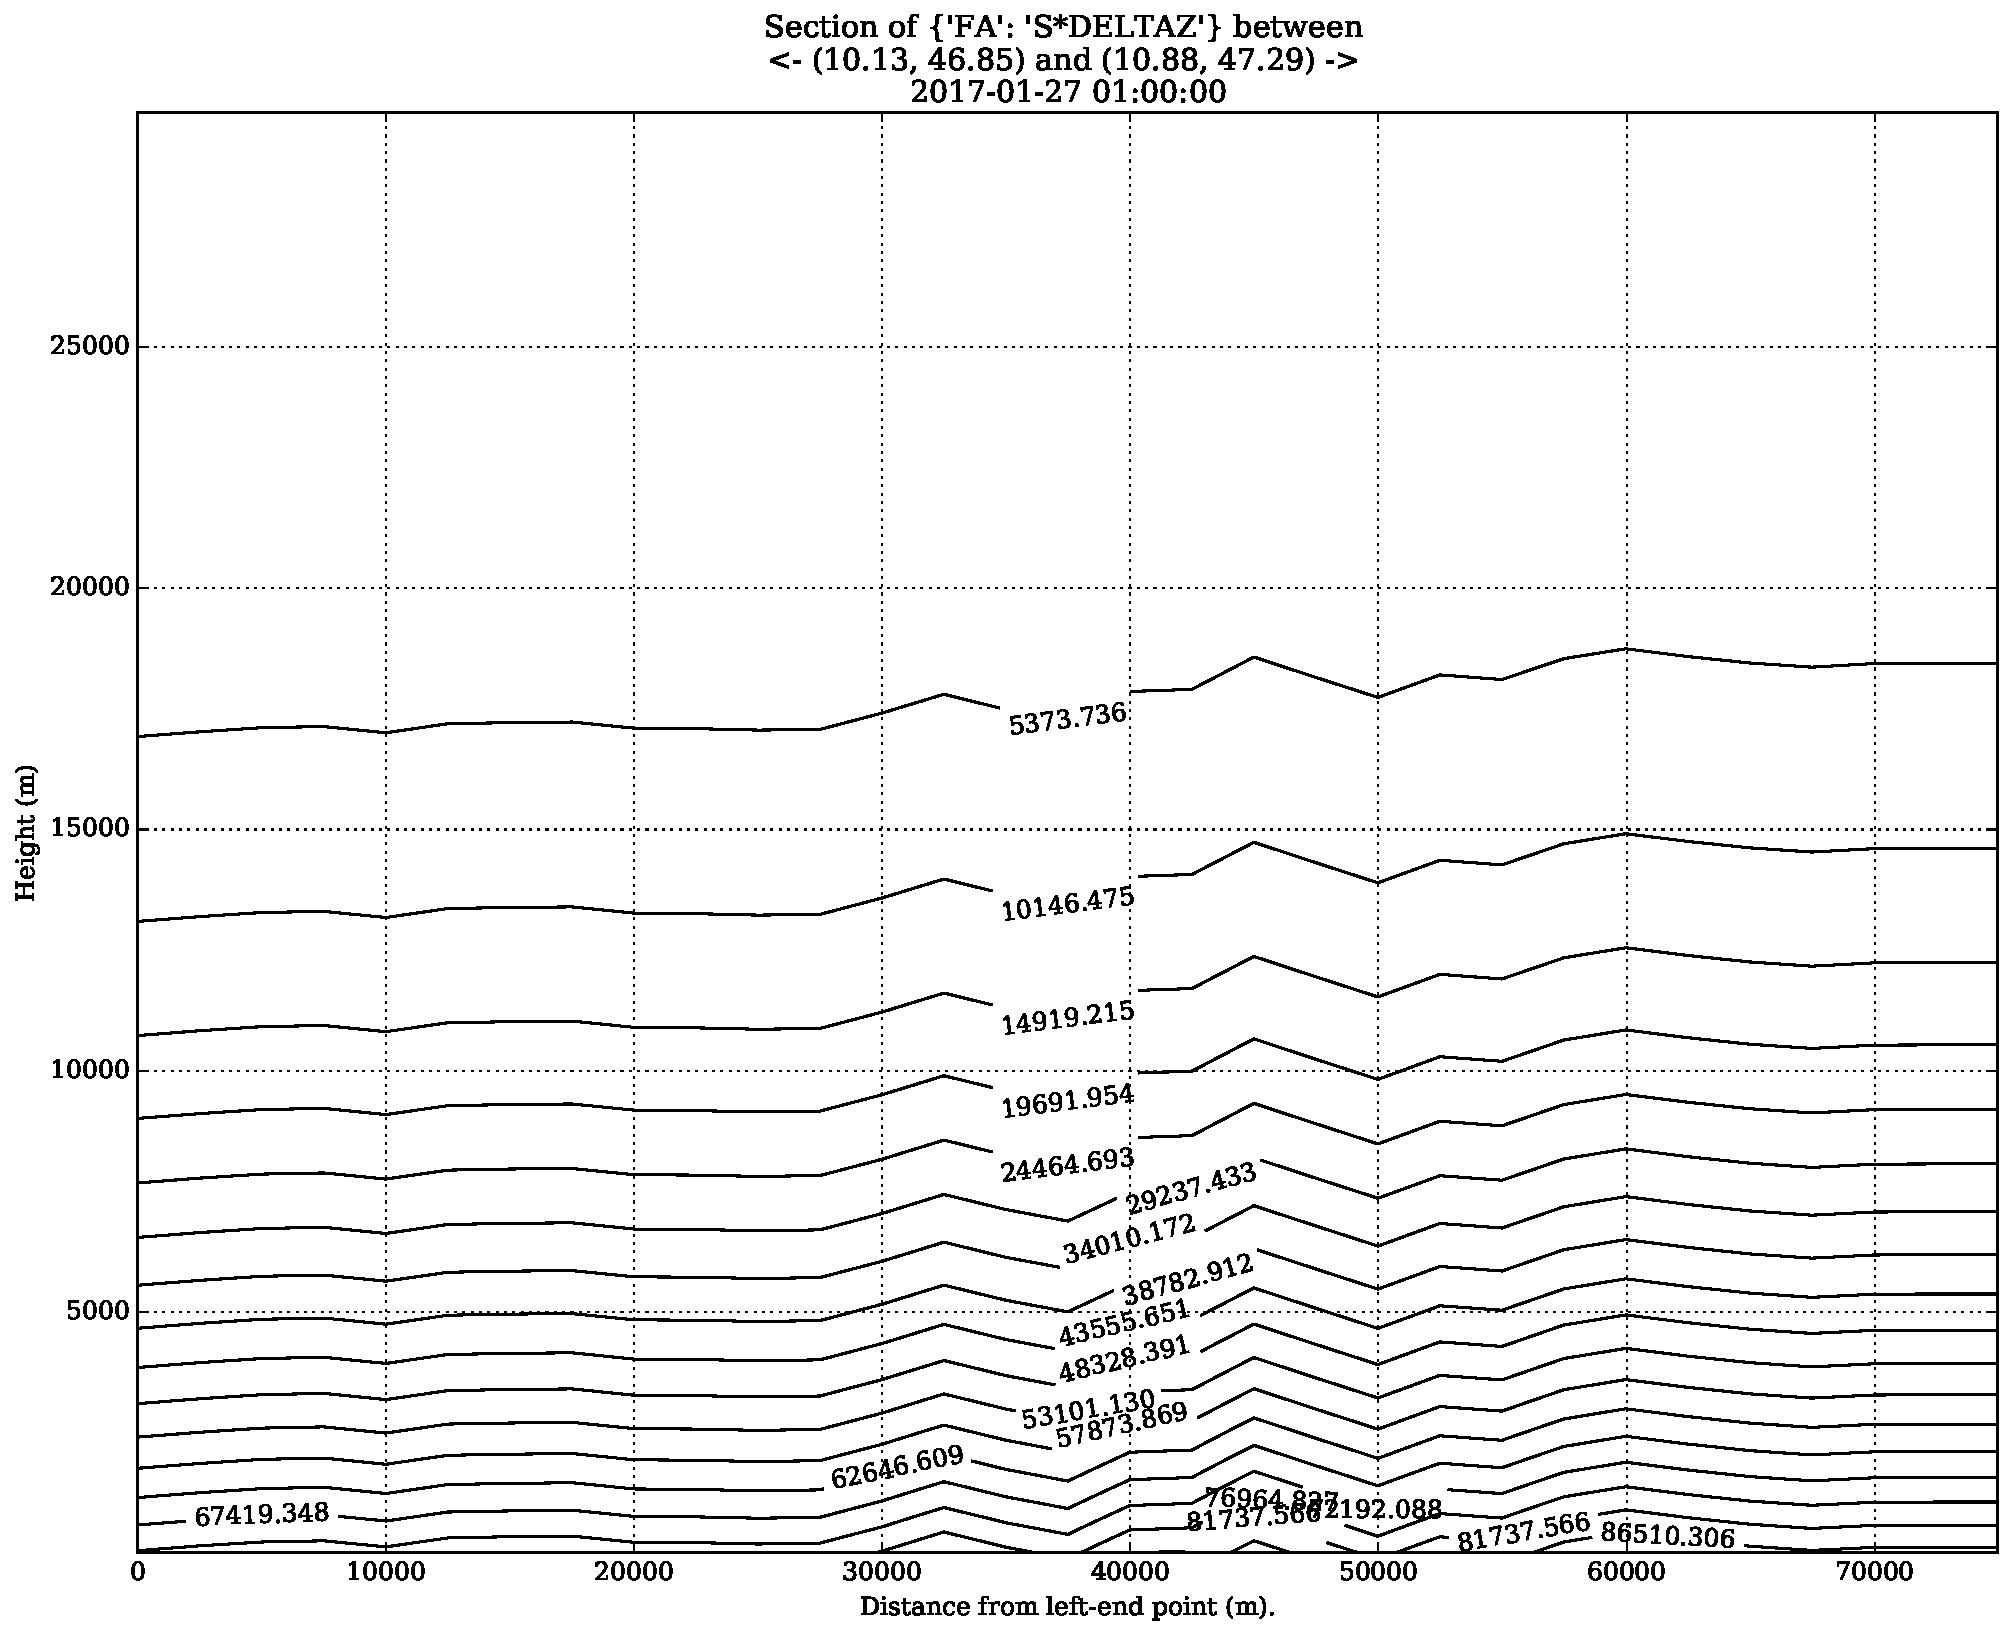
\includegraphics[trim={0cm 0cm  0cm  1.8cm },clip,width=\textwidth]{graphics/coordinates/PvsHeight.pdf}
    \caption{ \footnotesize{Terrain-following  coordinates: height above ground [m] on Y-axis}}
    \label{fig:PvsH}
    \end{subfigure}
    \hspace{1cm}
    \begin{subfigure}{0.45\textwidth}
    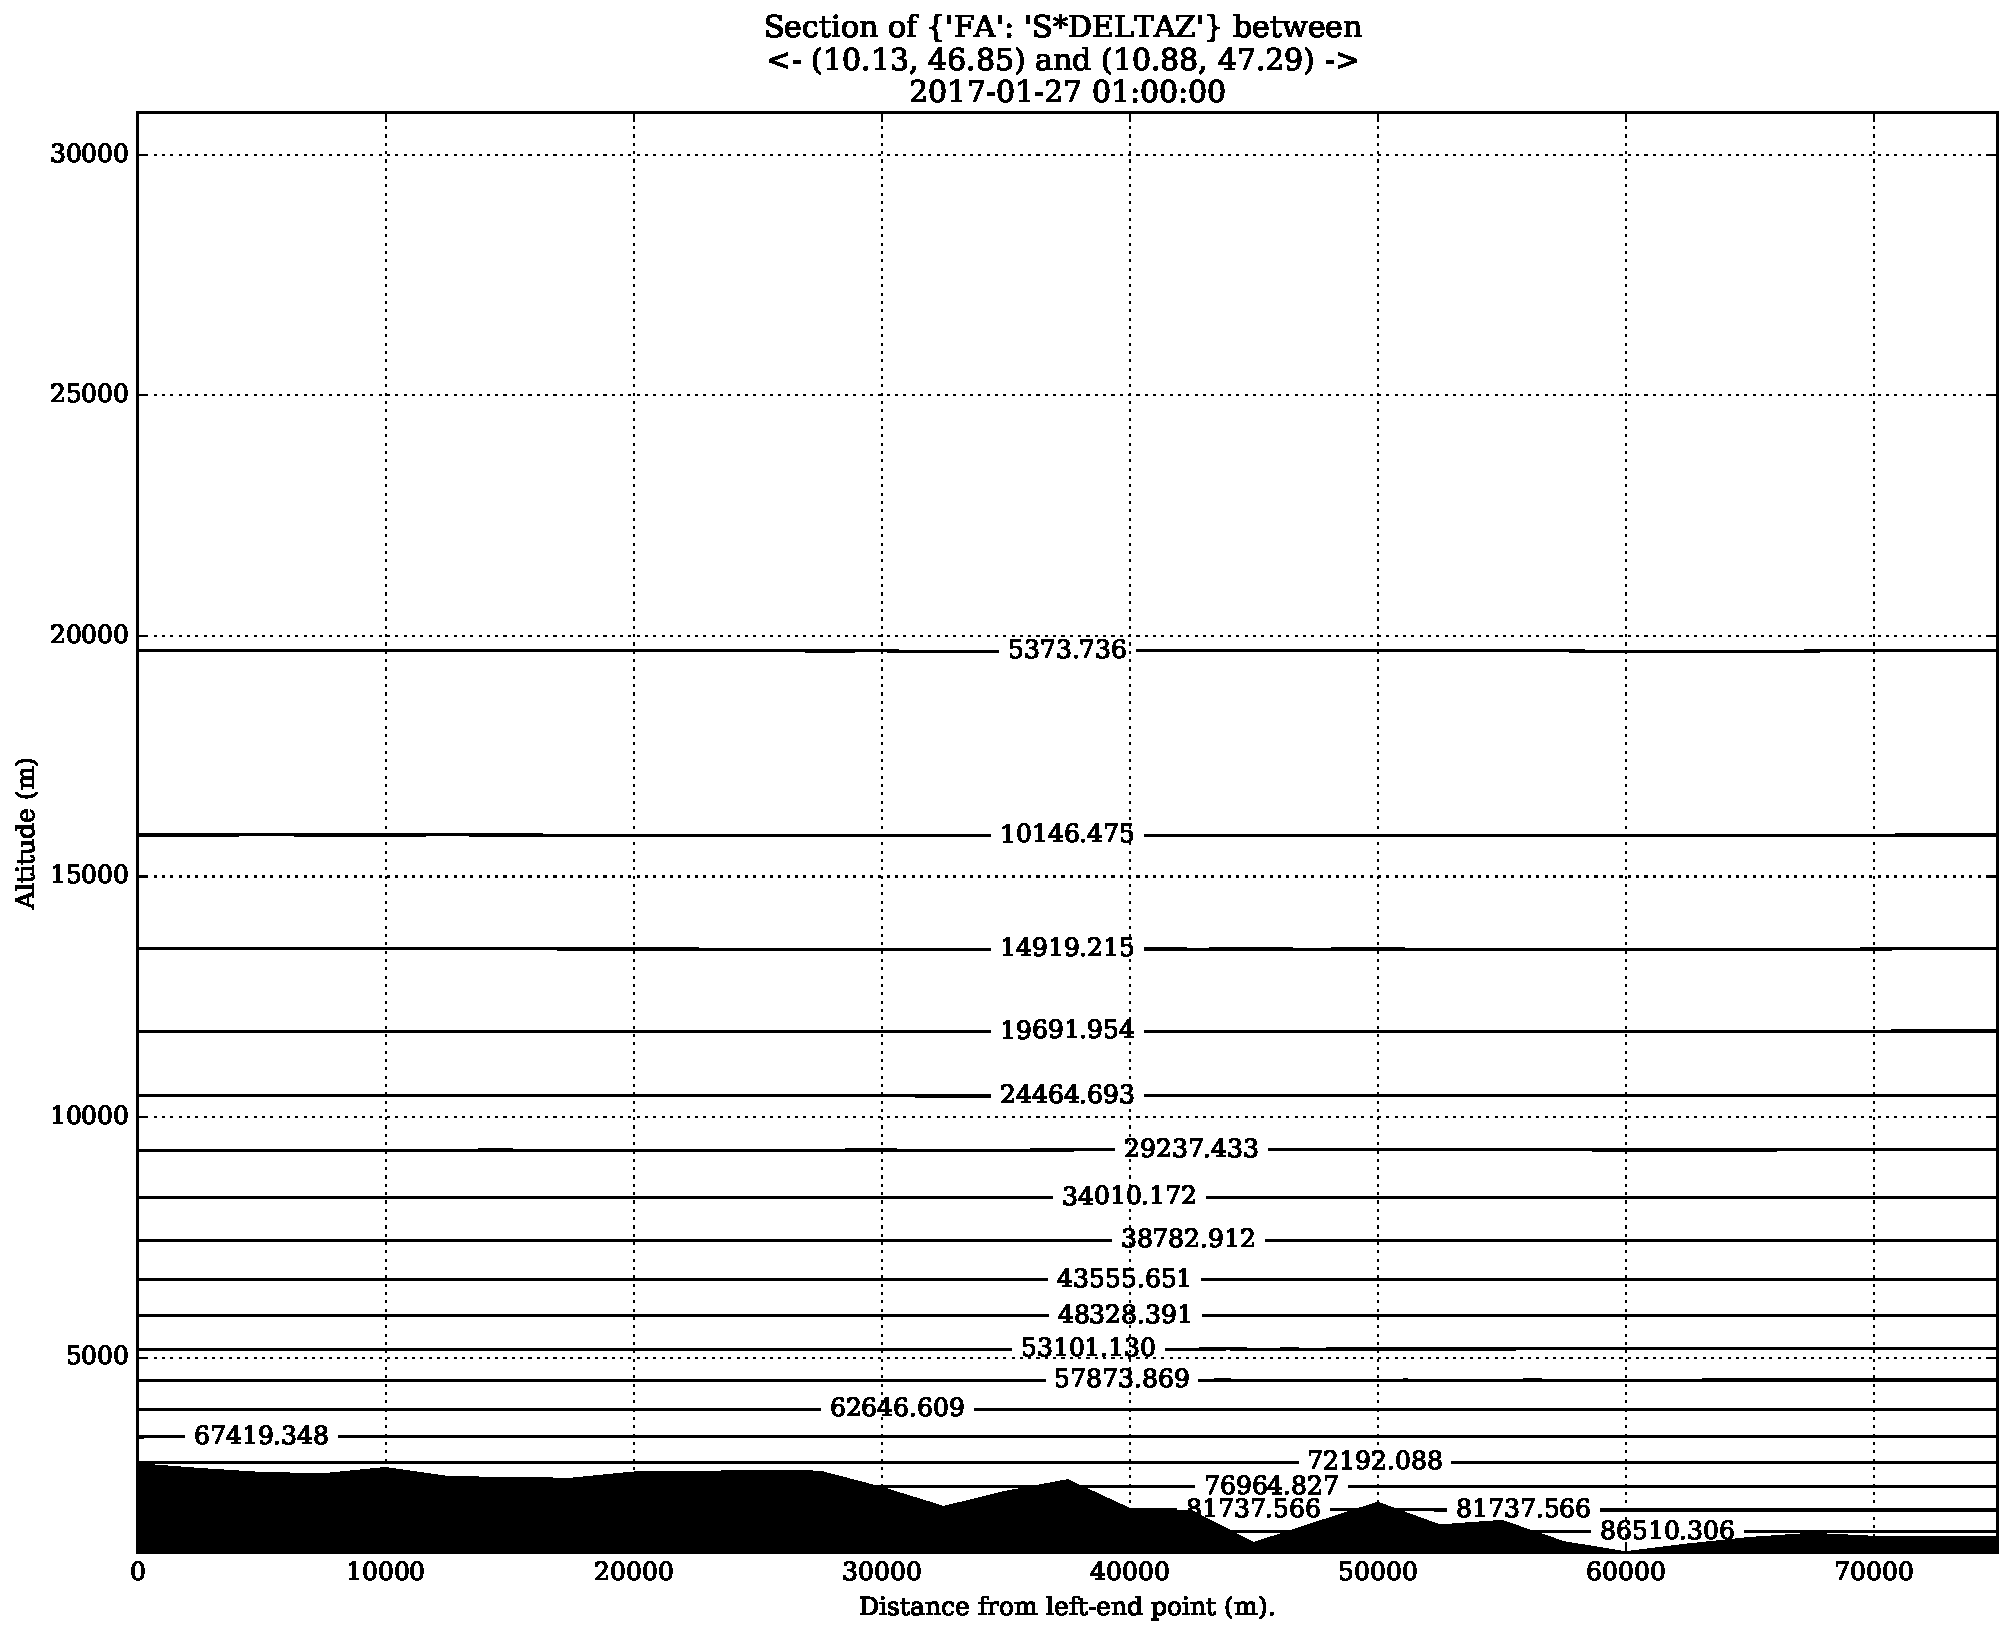
\includegraphics[trim={0cm 0cm  0cm  1.8cm },clip,width=\textwidth]{graphics/coordinates/PvsALtitude.pdf}
    \caption{\footnotesize{Traditional Height Coordinates: height above sea-level [m] on Y-axis}}
    \label{fig:PvsA}
    \end{subfigure}
    \caption[Comparison of Vertical Coordinate Systems]{Isobars in different vertical coordinate systems: 18 isobars (in [Pa]) of a cross section are shown in four different coordinate systems. The Y-axis is the vertical coordinate, different in each plot, and the X-axis is the horizontal distance from the starting point of the cross section. The cross sections starts at [lon:10.13, lat:46.85] (left end)  and ends at [lon:10.88, lat:47.29], showing a part of the Alps in western Austria to illustrate how topography is represented in different coordinate systems. Topological structures that cannot be a value assigned to are indicated as black surface.}
    \label{fig:coordinates}
\end{figure}
%draw simple figure to illustrate difference

\begin{figure}[p]
    \centering
    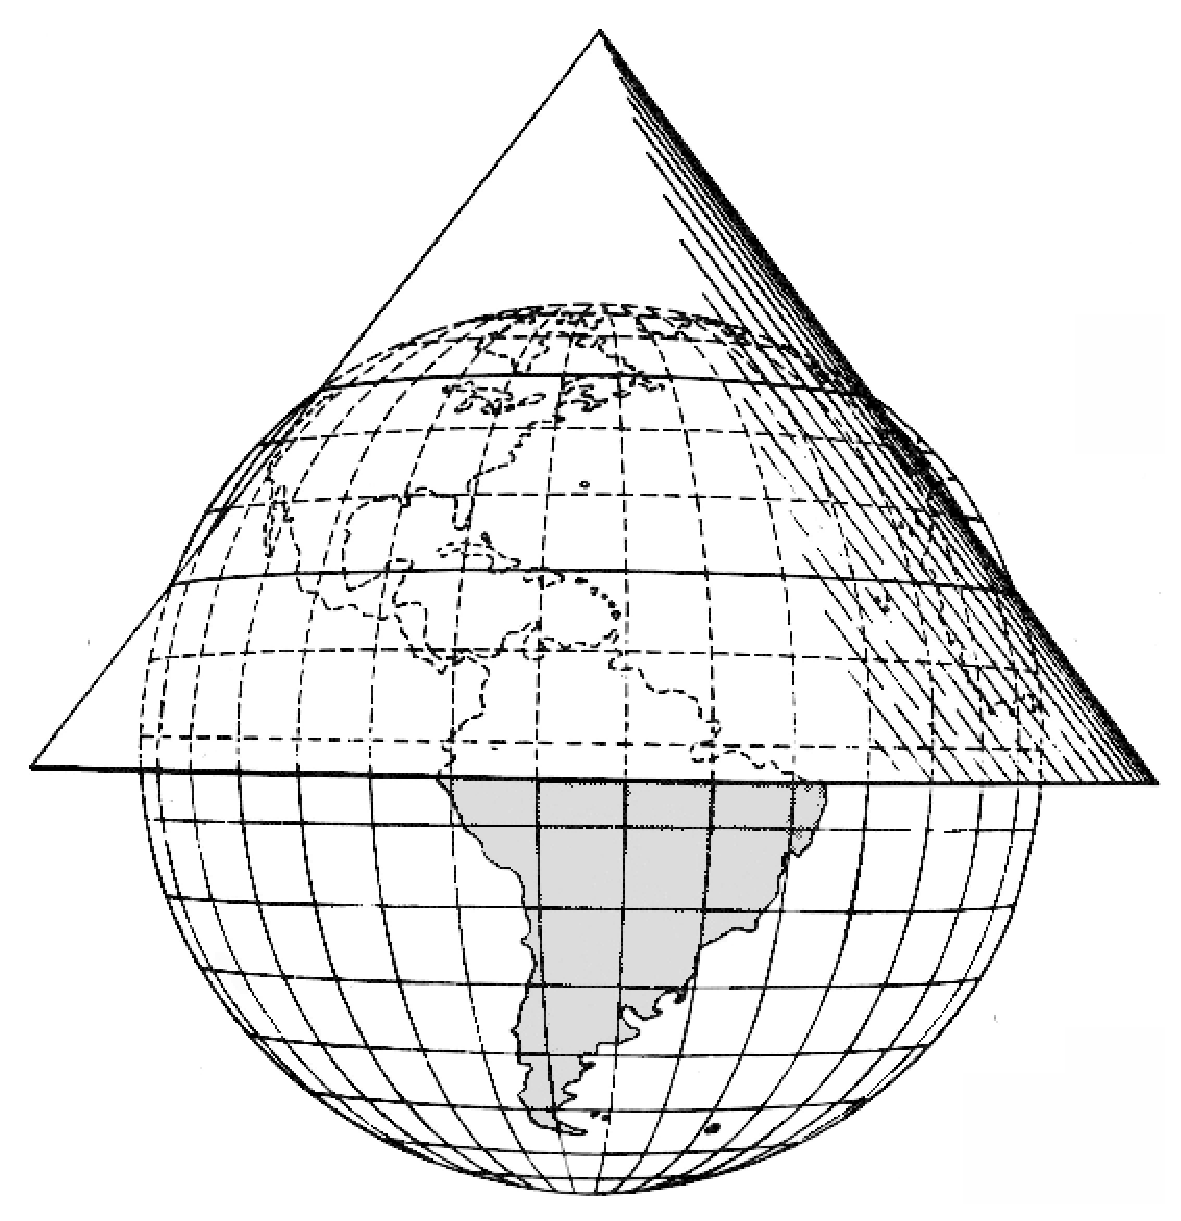
\includegraphics[width=\textwidth]{graphics/Lambert.eps}
    \caption[Lambert Projection]{Illustration of a conic conformal Lambert projection. Image by \citeauthor{usgs} \cite{usgs}}
    \label{fig:lambert}
\end{figure}
\newpage
\section{Pattern Generator}
\label{sec:pattern gen}
To perform Monte-Carlo forecasts by creating a stochastic physics ensemble a random number generator is needed. In most cases spatially and/or temporal correlations are necessary to represent realistic deviations from the deterministic scenario. To do so, a pattern generator that provides suitable randomly sampled spatial and temporal patterns, which can be applied to the relevant fields in the model, is the tool of choice.
In the AROME model the stochastic pattern generator generates a two-dimensional pattern, where the points are sampled from a normal distribution. Since the ranges of the quantities we want to perturb are restricted, the ranges of the perturbations need to be restricted as well.
Therefore a so-called clip ratio $x_{\mathrm{clip}}$ is defined in the namelist. Then, as described in the following by Equation \eqref{eq:fouriercoeff}, the distribution is cut off at the value of $x_{\mathrm{clip}}$ times the standard deviation $\sigma_{\mathrm{2D}}$. In this case `cut off' means, that if we define $a=x_{\mathrm{clip}} \sigma_{\mathrm{2D}}$, all sampled values outside the interval $[ -a, a] $ are set to $-a$ or respectively $a$.
This leads to the undesired result that the probability density function $f(p)$ does not have its minima, as desired at the edge of the mathematical domain. In fact, if the value for  $\sigma_{\mathrm{2D}}$ is too small, it can happen that the $f(p)$ has its maxima at the edges of the interval.

Another problem is that the pattern generator can only produce normal distributions. If the variable is suspected to be distributed differently, the only way to construct other distributions of randomly sampled numbers, is by use of the normally distributed pattern (e.g. taking the exponential of the numbers for lognormal distribution). Thus, one is severely limited in the selection of distribution. 

\subsection{Technical Set-Up of the Pattern Generator}

The pattern is constructed in spectral space and the corresponding coefficients $\hat{a}_{n,m}$, presented in Equation \eqref{eq:fouriercoeff}, are the coefficients of a double Fourier series. The pattern generator was originally implemented and described by \citeauthor{palmer2009stochastic} \cite{palmer2009stochastic} for the global ECMWF IFS model, where $\hat{a}_{n,m}$ relates to the spherical harmonics. The different coefficients are a consequence of the different representation of spectral fields in the ECMWF IFS and the AROME model. When the pattern generator is used on a LAM model the statistical properties of the fields are conserved, but the LAM fields are not congruent with the LAM domain of the global fields.\\
The spectral coefficients are obtained by random sampling and evolved by an auto-regressive process as described in Equation \eqref{eq:fouriercoeff}. 
\begin{equation}
\label{eq:fouriercoeff}
    \hat{a}_{n,m}(t+ \Delta t)= \Phi_{t} (t) \hat{a}_{n,m} +\sigma_{\mathrm{2D}}(n) \epsilon_{m,n} \Theta(x_{\mathrm{clip}}-\epsilon_{m,n})\Theta(\epsilon_{m,n} -x_{\mathrm{clip}})
\end{equation}
\begin{align*}
    \epsilon_{m,n} \in \mathbb{C}: \ 
 \Re(\epsilon_{m,n}) 
\sim N_{1}( \mu=0, \sigma=1); \  \
\Im(\epsilon_{m,n})
\sim N_{2}( \mu=0, \sigma=1)
\end{align*}

Here $ \Theta$ denotes the Heaviside step function which is defined as: 
\begin{flalign*}
&\Theta : \mathbb{R} \rightarrow \{ 0,1 \} \\
&x < 0: \Theta(x) = 0\\
&x \geq 0 : \Theta(x) =1\\ \quad .
\end{flalign*}
The random number generator samples the real and the imaginary part of  $\epsilon_{m,n}$ independently from a Gaussian distribution with variance $\sigma=1$ and mean $\mu=0$. $\epsilon_{m,n}$ is sampled independently for each $ m,n$ and $t$, where $n$ is the total wave number and $m$ is the zonal wave number, as defined in Equation \eqref{eq:zonalwavenumber}. The zonal wave number is the wave number for periodic boundary conditions at a given latitude $\phi$
\begin{equation}
m \lambda=2 \pi R_{\mathrm{E}} cos(\phi) \quad ,
\label{eq:zonalwavenumber}
\end{equation}

where $R_{\mathrm{E}}$ is the Earth's radius, $\phi$ the latitude and $\lambda$ the wavelength. Then the sample gets cut off below and above the clip ratio  $x_{\mathrm{clip}}$  and scaled by $\sigma_{\mathrm{2D}}(n)$.



Each  pattern $\Psi$ is characterized by its spatial correlation $ L_{\Psi}$ and its temporal correlation $ \tau_{\Psi}$, because those two parameters determine $\Phi_{\mathrm{t}} (t)$ and $\sigma_{\mathrm{2D}}(n)$ which define the spectral coefficients of the pattern, as demonstrated by Equation \eqref{eq:fouriercoeff}. The dependencies of  $\Phi_{t} (t)$ and $\sigma_{\mathrm{2D}}(n)$ on the correlation scales are non-linear and defined as the following:\\
\begin{equation}
    \Phi_{t} = \exp \left( \frac{ - \Delta t}{\tau_{ \Psi}} \right)
\end{equation}
\begin{equation}
    \sigma_{\mathrm{2D}}(n) = F_{0} \ \chi(n)
    \label{eq:std}
\end{equation}
\begin{equation}
    F_{0}=\frac{\sqrt{1 - \Phi_{t}^2} \ \sigma_{\mathrm{nl}}}{ \gamma}  
\end{equation}
\begin{equation}
    \chi =  \exp (-0.5 \  \zeta \  n \ (n+1))
\end{equation}
\begin{equation}
\zeta = 0.5 \left( \frac{L_{\Psi}}{R_{\mathrm{E}}} \right)^{2}
\end{equation}
\begin{equation}
    \gamma = \sum_{n} \sqrt{2n +1} \ \chi (n)
\end{equation}
The scaling parameters $\Phi_{t} (t)$, $ L_{\Psi}$, $x_{\mathrm{clip}}$ and $\sigma_{\mathrm{nl}}$ (relates to the variance of the distribution) are all set in the model configuration, called namelist hereafter.
\begin{figure}[h]
\captionsetup{width=.7\linewidth}
    \centering
    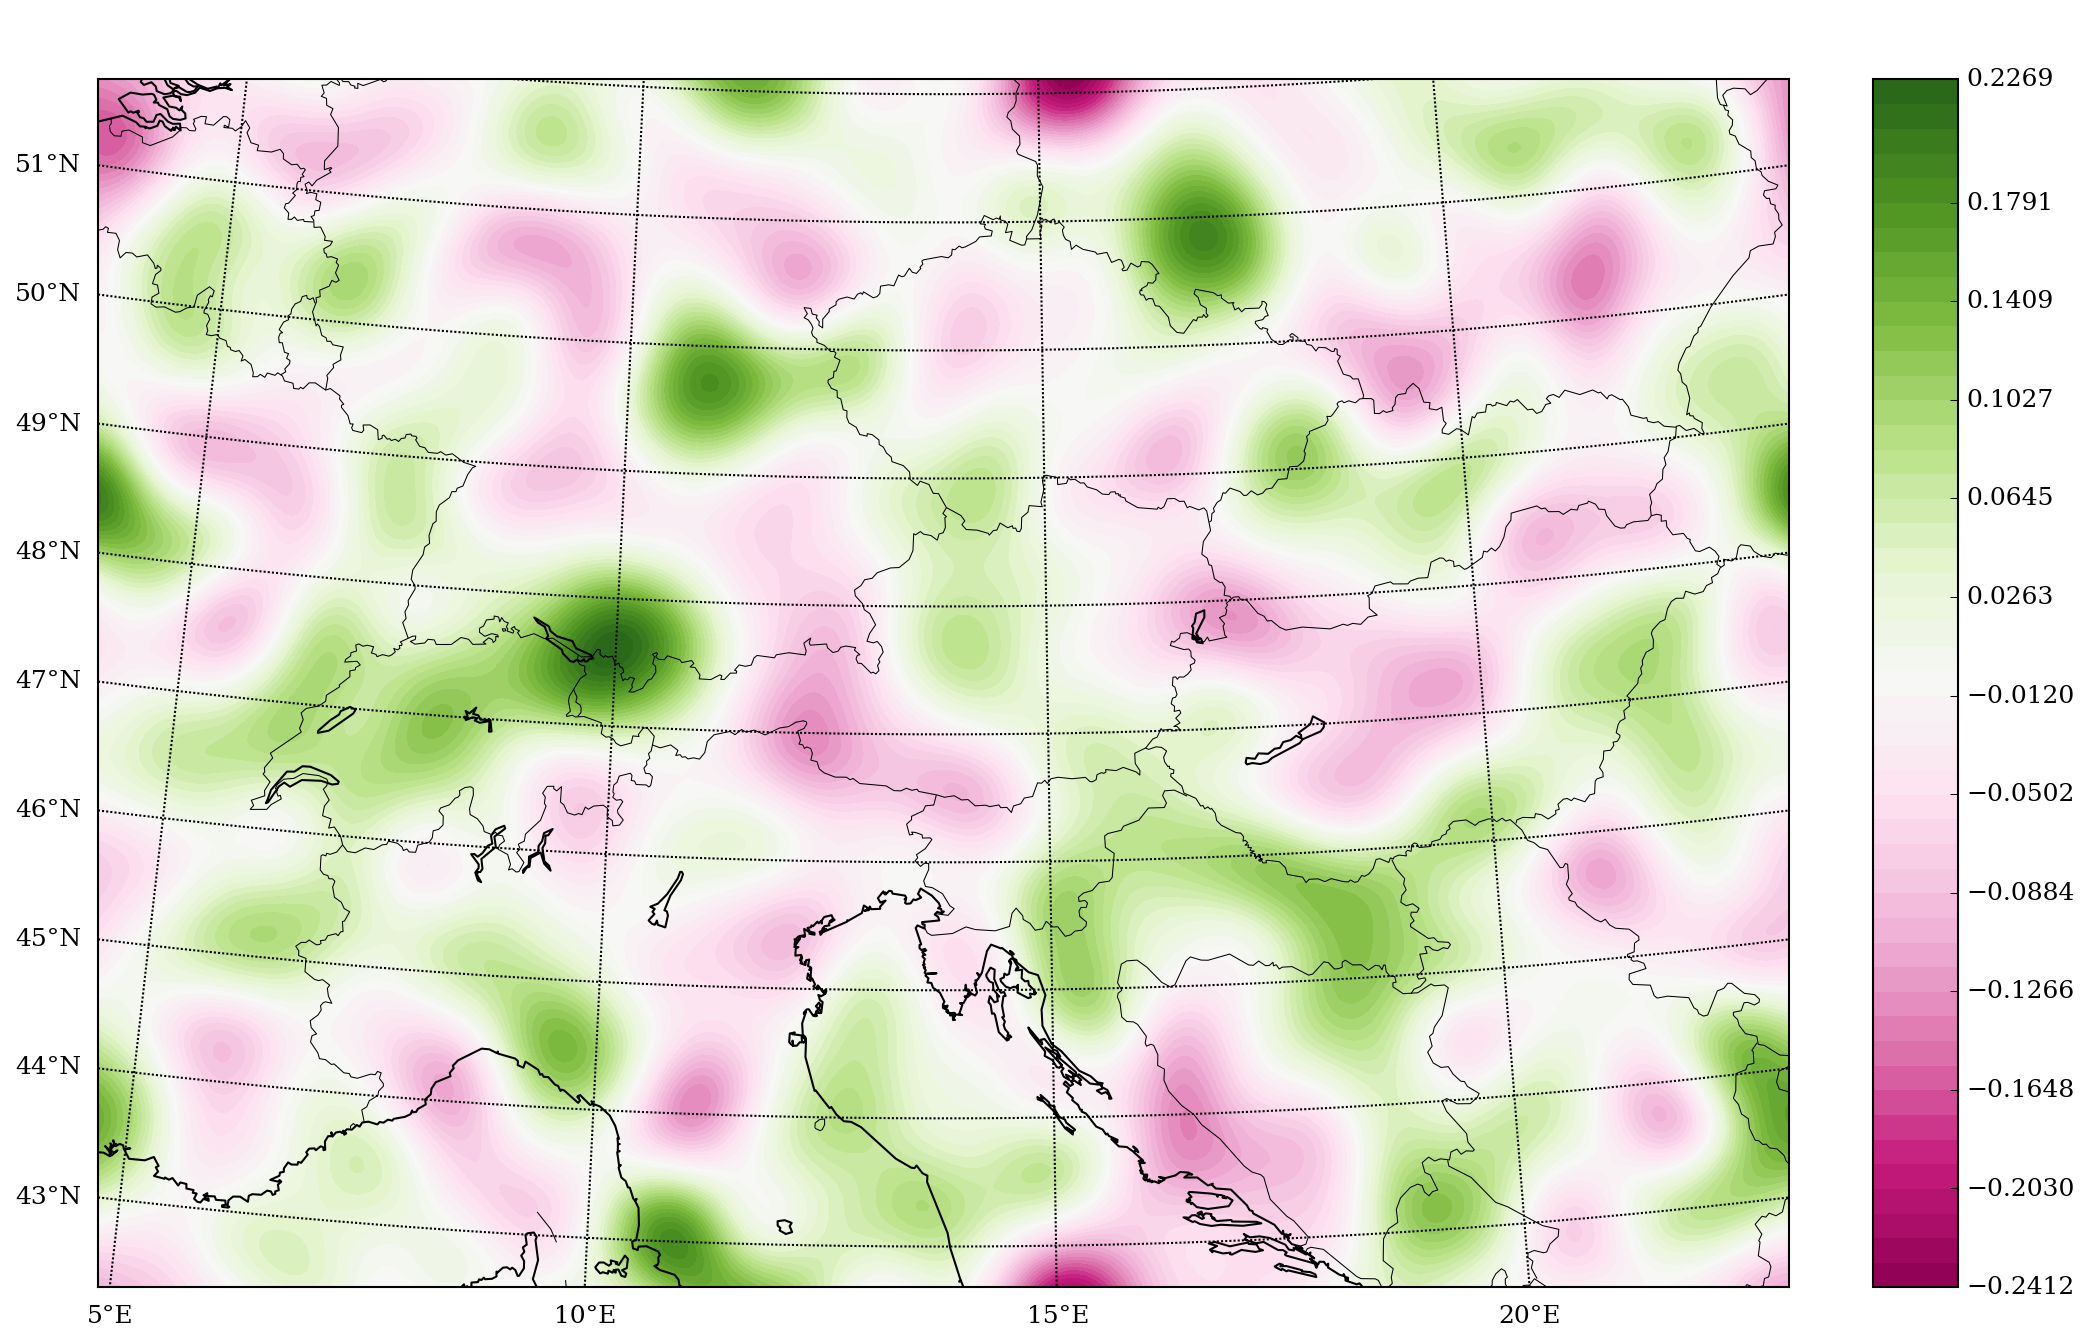
\includegraphics[width=0.7\textwidth]{graphics/mesoscale-pert.png}
    \caption[Example of a Small-Scale Perturbation]{Example of a normally distributed small-scale perturbation generated by the pattern generator}
    \label{fig:example-pert}
\end{figure}


\chapter{Parametrization of Visibility}

\label{sec:param}
For the newly introduced parametrization, two different existing approaches are merged:
One for Mie scattering by hydrated aerosols introduced by \citeauthor{clark2008prediction} \cite{clark2008prediction} and the other one by \citeauthor{stoelinga1999nonhydrostatic} \cite{stoelinga1999nonhydrostatic}, where the parametrization of the extinction coefficient is directly dependent on the mass concentration of snow, rain, cloud water and cloud ice.\\
This `merged' parametrization is called `Clark+' hereafter and is defined as 
\begin{equation}
    vis  = - \ln ( \varepsilon) \left( \beta_{R} + \sum\limits_{i=1}^{N_{h}} \beta_{h,i} +  \sum\limits_{j=1}^{N_{a}} \beta_{a,j} \right) ^{-1} \quad ,
\end{equation}
%describer surface volume coefficients in general 
where $N_{h}$ denotes the number of different species of hydrometeors. Usually hydrometeor means all forms of precipitation, but in this case we will not only call snow and rain  hydrometeors, but  liquid cloud water and cloud ice too, to be consistent with nomenclature in the models. The number of different aerosol species is denoted by $N_{{a}}$. In general, an aerosol is defined as air with suspended particles, but in meteorological terminology the term aerosols only refers to the particles in the suspension, excluding hydrometeors \cite{raith2001erde}.
The extinction coefficients of the different hydrometeors are taken from the parametrization by \citeauthor{stoelinga1999nonhydrostatic} \cite{stoelinga1999nonhydrostatic}, who refer to \citeauthor{rutledge1983mesoscale} \cite{rutledge1983mesoscale} and \citeauthor{kunkel1984parameterization} \cite{kunkel1984parameterization}, who define them as
\begin{equation}
\beta_{h,i} = a_{0,i} \ (c_{i} \ \rho \times 10^{3})^{a_{1,i}} \quad , \\
\end{equation}
where $c_{i}$ stands for the mass concentration of the hydrometeors and $\rho$ for the density of air. In general the coefficients $a_{0,i}$ and  $a_{1,i}$, shown in Table \ref{tab:Surface-Volume-Coefficients}, are related to the surface-volume-ratio of a hydrometeor. That is because the larger the surface-to-volume ratio of a hydrometeor is, the more likely is the light to be scattered for the same mass concentration ( e.g. a snowflake has a higher extinction efficiency than a water drop).\\
\begin{table}[]
    \centering
    \begin{tabular}{|l|c|c|}
    \hline
    \multicolumn{3}{|c|}{\textbf{Surface-Volume-Coefficients}}\\
    \hline
    \textbf{Type of Hydrometeor} & $\boldsymbol{a_{0,i}}$ & $\boldsymbol{a_{1,i}}$\\
    \hline
        rain & 1.1&0.75 \\
    \hline
        snow& 10.4& 0.78\\
    \hline
        liquid cloud water&144.7 & 0.88\\
    \hline
        cloud ice & 1.1& 1\\
    \hline
    \end{tabular}
    \caption{Surface-Volume-Coefficients}
    \label{tab:Surface-Volume-Coefficients}
\end{table}
The extinction coefficients of the different aerosols $\beta_{\mathrm{a},j}$ depend mainly on the mass attenuation coefficients $\alpha_{j}$ of the aerosols:
\begin{equation}
    \beta_{a,j} = \alpha_{j} (q_{\mathrm{rel}}(q_{\mathrm{spec}}, T ,p))  \ c_{j} \  \rho_{\mathrm{dry}} \quad .
\end{equation}

As $\alpha_{j}(q_{\mathrm{rel}}(q_{\mathrm{spec}}, T ,p)$ implies, $\beta_{\mathrm{a},j}$ depends also on the humidity. The reason being, that the particles' sizes and therefore the scatter properties of aerosols, are affected by hygroscopic growth \cite{lang2010interaction}, which is considered in the parametrization. \\
In the parametrization five different aerosol species are considered: sea salt, desert dust, black carbon, organic matter and sulphates. From these five aerosols only sea salt, sulphates and organic matter undergo hygroscopic growth and it can be neglected for desert dust and black carbon, due to their predominantly hydrophobic chemical composition. The mass attenuation coefficients, presented in Table \ref{tab:absorption}, are gained from a Mie scattering algorithm implemented and described by \citeauthor{reddy2005estimates} \cite{reddy2005estimates} and take the humidity into account by adapting the particle radius and the mass attenuation. All values were chosen for the wavelength of 555nm for the incoming light, because the human eye has a peak in sensitivity at this wavelength \parencite{horvath1981atmospheric, WMO}.\\
The contrast threshold $\varepsilon$ determines when an object is considered to be visible. As discussed in Section \ref{sec:visib}  different values have been used in the past, but in agreement with  \citeauthor{clark2008prediction} \cite{clark2008prediction} it was set to $2 \% $ for this study.\\
The layers which are used for calculating the average visibility can be set, depending on the purpose of the forecast. The default values, also used for this study, are set to average over the lowest 10 layers. This corresponds to a height from 0 to 240 \textendash 300m above the ground. The range of the upper boundary is due to the horizontal variation of the maximum height within one layer caused by the usage of hybrid-pressure-terrain-following coordinates (see Figure \ref{fig:coordinates}.\\
The data of the aerosol concentration and its spatial distribution are taken from the NASA database [\citeurl{nasa}]. This aerosol data set was generated by simulating sinks and sources of different aerosols according to the works of  \citeauthor{tegen1997contribution} \cite{tegen1997contribution}, \citeauthor{chin1996global} \cite{chin1996global}, \citeauthor{liousse1996global} \cite{liousse1996global} and \citeauthor{tegen1995contribution} \cite{tegen1995contribution}, and is a climatological data set. Thus, high accuracy and currentness of the data is not given. This increases the uncertainty in the visibility parametrization. The aerosols data is provided in the unit of optical depth. To calculate the mass concentration the scattering cross section, a reference height and the density of air is needed. The scattering cross sections are also included in the NASA data set \cite{nasa} and reference height in the corresponding works \cite{tegen1997contribution,chin1996global, liousse1996global,tegen1995contribution}.\\
The extinction coefficient of the Rayleigh contribution represents the scattering by atmospheric gases. As suggested by \citeauthor{clark2008prediction} \cite{clark2008prediction} it was set to $\beta_{R}$ = 0.0391, the equivalent of 100km visibility.\\
Since so many physical processes that contribute to visibility cannot be resolved explicitly, there are many different approaches of parametrizing visibility \cite{claxton2008using, clark2008prediction, smirnova2000case, stoelinga1999nonhydrostatic, gultepe2010probabilistic,gultepe2006, chmielecki2011probabilistic}.
The simplest and computationally least expensive way to forecast visibility is to find an analytical function of some model variables by fitting to a set of measured data.\\
For benchmarking, seven other parametrizations of that kind were implemented, which were gathered from  \citeauthor{gultepe2010probabilistic} \cite{gultepe2010probabilistic} and \citeauthor{ gultepe2006} \cite{ gultepe2006} and are presented in Table \ref{tab:Paraoverview}.


\begin{landscape}
    \renewcommand{\arraystretch}{2.5}
    \begin{table}[p]
        \centering
        \begin{tabular}{|l|c|r|}
            \hline
             \textbf{Abbreviation}&  \textbf{Reference}& \textbf{Parametrization}\\
             \hline
             Gul&\citeauthor{gultepe2006}(\citeyear{gultepe2006}) \cite{gultepe2006}, post-processing & $ \mathrm{min} \left[ 0.0219*\mathrm{LWC}^{-0.9603} \times 10^{-3}, \  67700* (1 - q_{\mathrm{rel}} ) ^ {0.67} \times 10^{-3} \right] $\\
             \hline
             Clark+& \citeauthor{clark2008prediction}  (\citeyear{clark2008prediction})\cite{clark2008prediction}, \citeauthor{stoelinga1999nonhydrostatic}(\citeyear{stoelinga1999nonhydrostatic})\cite{stoelinga1999nonhydrostatic}& $ -ln ( \epsilon) \left( \beta_{R} + \sum_{i}^{N_\mathrm{hydro}} \beta_{\mathrm{hydro},i} +  \sum_{j}^{N_\mathrm{aero}} \beta_{\mathrm{aero},j} \right)^{-1}$\\
             \hline
             RUC & \citeauthor{smirnova2000case}(\citeyear{smirnova2000case})\cite{smirnova2000case}& $ 60 \exp \left( \frac{- 2.5 \left( q_\mathrm{rel} \times  10^{2}-15 \right) } {80} \right)$\\
             \hline
             FRAMC &\citeauthor{gultepe2006}(\citeyear{gultepe2006})\cite{gultepe2006}& $ -41.5 \ln \left(  q_\mathrm{rel}\times 10^{2}\right) + 192.3 $\\
             \hline
             AIRS & \citeauthor{gultepe2006}(\citeyear{gultepe2006})\cite{gultepe2006}& $ -0.0177 \left( q_\mathrm{rel}\times 10^{2} \right) ^{2} + 1.46q_\mathrm{rel} +30.80$\\
             \hline
             FRAML5 &\citeauthor{gultepe2010probabilistic}(\citeyear{gultepe2010probabilistic})\cite{gultepe2010probabilistic}&  $ -0.000114  \left( q_\mathrm{rel}\times 10^{2} \right)^{2.7} + 27.45 $\\
             \hline
             FRAML50 & \citeauthor{gultepe2010probabilistic}(\citeyear{gultepe2010probabilistic})\cite{gultepe2010probabilistic}& $ -5.19 \times 10^{-10}  \left( q_\mathrm{rel}\times 10^{2} \right)^{5.44} + 40.10$\\
             \hline
             FRAML95 & \citeauthor{gultepe2010probabilistic}(\citeyear{gultepe2010probabilistic})\cite{gultepe2010probabilistic}& $-9.68 \times 10^{-14}  \left( q_\mathrm{rel}\times 10^{2} \right)^{7.19} + 52.20 $\\
             \hline
             
        \end{tabular}
        \caption{Overview of all implemented parametrizations, including references and used abbreviations. }
        \label{tab:Paraoverview}
    \end{table}
\end{landscape}
\begin{landscape}
    \renewcommand{\arraystretch}{1.5}
    \begin{table}[H]
 %   \fontsize{9}{9}\selectfont
    \begin{adjustbox}{width=1.5\textwidth,center}
        \begin{tabular}{|l|c|c|c|c|c|c|c|c|c|c|c|c|}
        \hline 
        \multicolumn{13}{|c|}{  \textbf{Mass Attenuation Coefficients of Different Aerosols } $\boldsymbol{\alpha_{j} [m^2/g]}$ }\\
        \hline 
         \textbf{Relative Humidity} &\textbf{0.0}&\textbf{0.1}&\textbf{0.2}&\textbf{0.3}&\textbf{0.4}&\textbf{0.5}&\textbf{0.6}&\textbf{0.7}&\textbf{0.8}&\textbf{0.85}&\textbf{0.9}&\textbf{0.95}\\
        \hline 
        Sulphates&4.94247&4.94247&4.94247&4.94247&6.85&7.74471&8.92815&10.6356&13.5782&16.2277&21.0072&35.4261 \\
        \hline
        Organic Matter&3.07043&3.07043&3.07043&3.07043&4.27185&4.84567&5.60681&6.70989&8.6229&10.3565&13.5060&23.1454\\
        \hline
        Sea Salt&0.03889&0.03889&0.03889&0.03889&0.07921&0.09226&0.10549&0.122930&0.149650&0.17160&0.21005&0.31026 \\
        \hline
        Desert Dust& \multicolumn{12}{c|}{0.42744}\\
        \hline
        Black Carbon &  \multicolumn{12}{c|}{9.412290}\\
        \hline
        \end{tabular}
    \end{adjustbox}
    \caption{List of mass attenuation coefficients of different aerosols. Sulphates, organic matter and sea salt undergo hygroscopic growth and resulting in a different mass attenuation for different values of relative humidity. The relative humidity is categorized in different bins. The values shown in this table, starting from the left to the right, denoting the edges of the bins. The upper edge of the last bin is missing, obviously being 1. } \label{tab:absorption}
    \end{table}

\end{landscape}


%Use graph with 
\chapter{Methods and Set-Up}
\label{sec:methods}
\section{Perturbation Scheme}
\begin{figure}
    \centering
    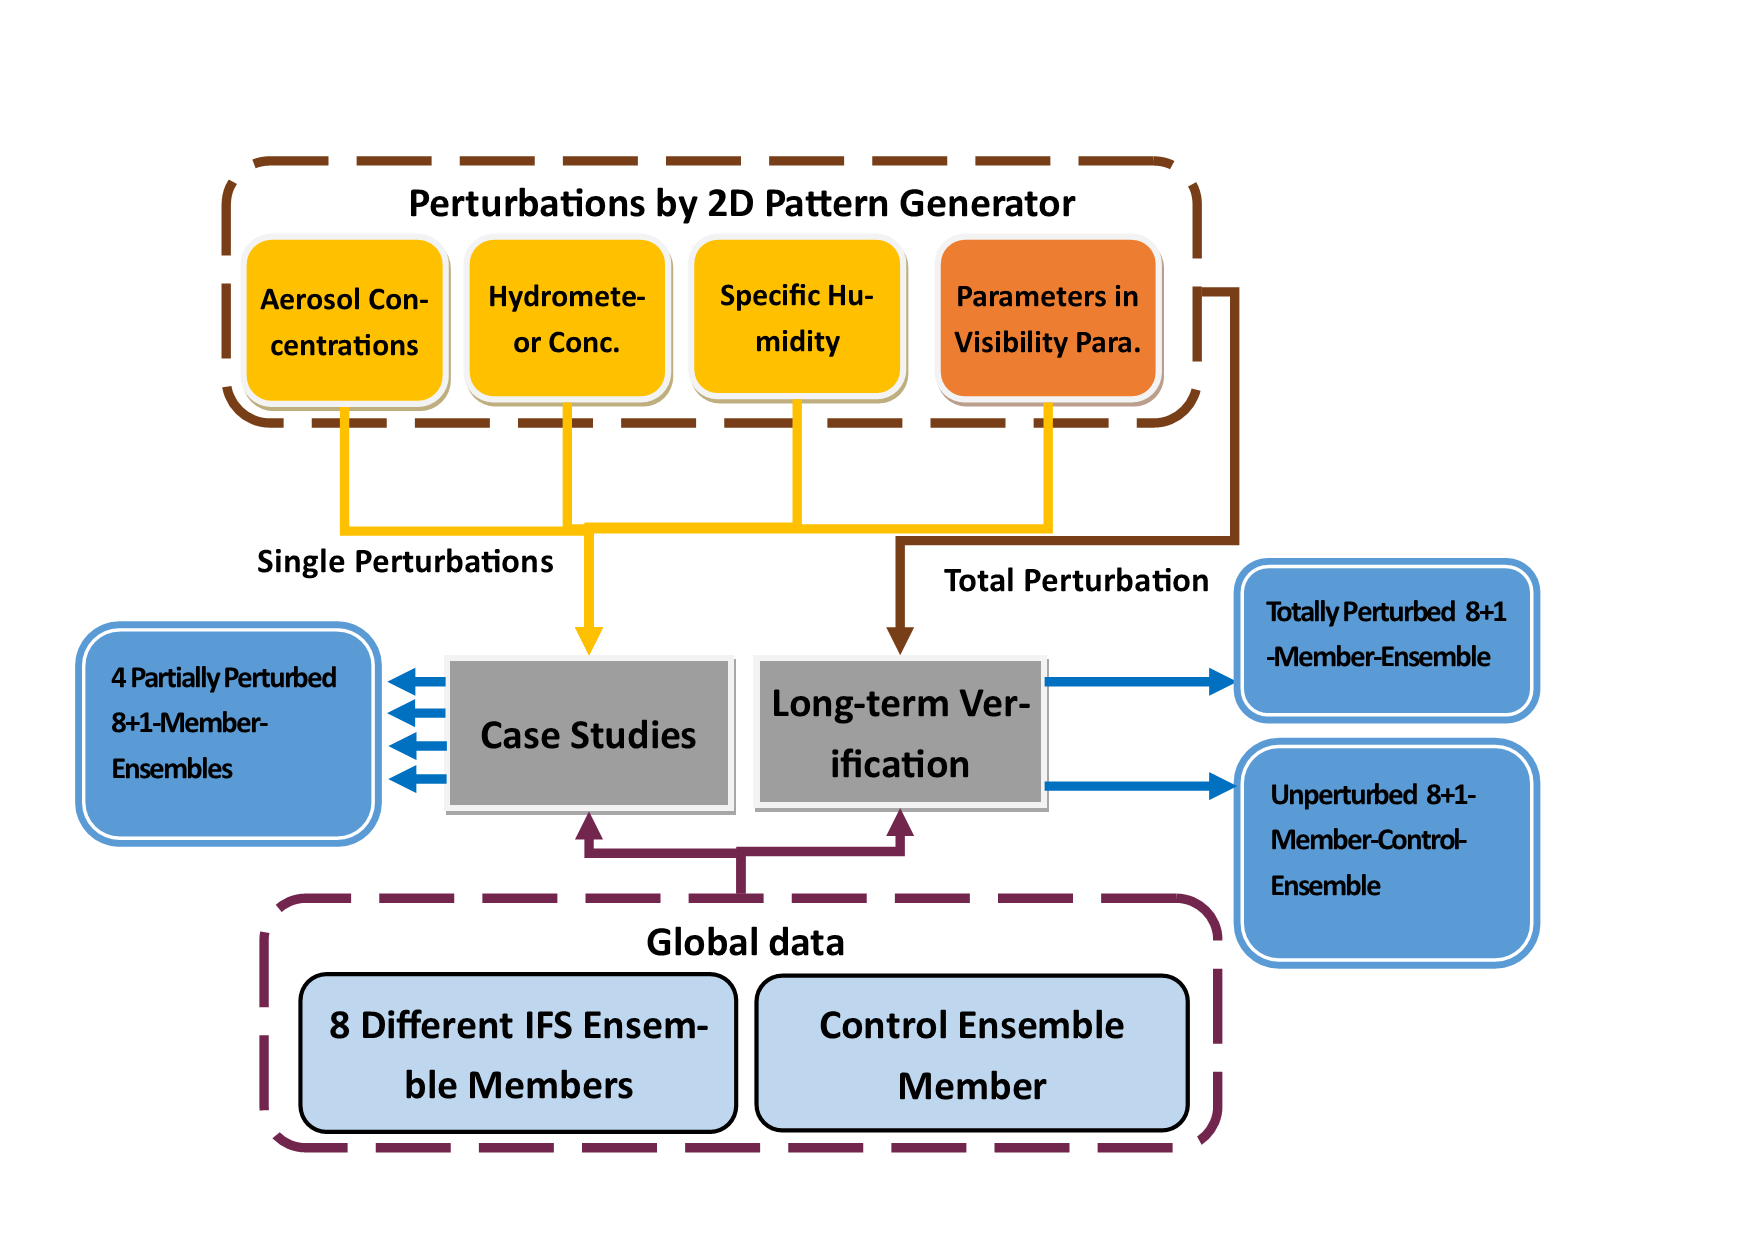
\includegraphics[width=\textwidth]{graphics/Perturbationsscheme.png}
    \caption[Illustration of Perturbation Scheme]{Illustration of the perturbation scheme: Showing the different perturbed quantities at the top and the used ensemble members from the IFS model on bottom. }
    \label{fig:pertrubation_scheme}
\end{figure}
For the evaluation of the parametrization, several forecasts with different perturbation schemes, also called NWP experiments, were performed.
To investigate the influence of different variables on visibility, the following versions of perturbations, presented in Figure \ref{fig:pertrubation_scheme}, were tested:
\begin{enumerate}
    \item{Control ensemble}
    \item {Perturbation of aerosol concentrations}
    \item {Perturbation of hydrometeors}
    \item {Perturbation of the parameters in the visibility parametrization}
    \item {Perturbation of specific humidity}
    \item {Total perturbation (aerosols, hydrometeors, specific humidity, parameters) }
    
\end{enumerate}
Figure \ref{fig:pertrubation_scheme} illustrates the listed perturbed variables and which combinations were run as case studies and for the long-term verification. No additional perturbation was applied to the control ensemble. It constitutes of an AROME ensemble, which was created by using data of eight perturbed members and one control member of the IFS ensemble to set different boundary and initial conditions for each member. The measured visibility lies often outside the ensemble spread of the control ensemble, mainly, because this ensemble does not take model error into account. Especially for visibility, many of the key parameters are hard to predict reliably and often not varied in the standard perturbation schemes \cite{chmielecki2011probabilistic}. To tackle this underdispersion of the control ensemble, additional local perturbations were introduced.\\
In this case, local means, the perturbations were chosen and set-up to be applied only in the visibility module. The other parts of the model remained untouched. \\
For the perturbed ensemble, the current values are perturbed with the corresponding spatial-temporal pattern  at each time step and the perturbed quantities are passed on to the visibility parametrization and thus, do not affect any future states of the model. This method forbids the perturbations to be amplified in time, and therefore the default amplitudes must be higher in comparison to a perturbation scheme that is applied to the overall model and can evolve.
The reason why a local perturbation scheme is used, is that no global perturbation scheme for AROME is available, where all the relevant parameters and variables can be perturbed.
Perturbing all of them globally, would lead to a change in a number of non-linear feedback processes. The model could not handle those perturbations, because the effects of different perturbations can have conflicting outcomes for different variables. Since we are only interested in investigating the uncertainty of the visibility forecast, a local perturbation is sufficient.\\
Although we can estimate the ranges for all parameters quite well, we have very little a priori knowledge about the compatibility of the values of different variables after a certain time.\\
For a locally applied perturbation, the distance to the original trajectory in phase space can be restricted and chosen small enough to have tolerable errors. If we would allow them to propagate, we are unable to predict how the perturbed trajectory will evolve. There is no guarantee that it will lead to a realistic outcome at a later time, because the tolerable error can be amplified to a completely nonsensical scenario. 
There are several other attempts of probabilistic forecasting of visibility \cite{chmielecki2011probabilistic, Roquelaure}, but we believe that the advantage of our method is its comprehensible nature. It is not purely statistical but relates to single physical quantities.\\

The details of the perturbation scheme are outlined in the following subsections.
%Aufzehulgn jeder ienzelnen Storung und Beschreibung der range einschraenkung

\subsection{Set-Up of Perturbations}
All perturbations were generated by use of the pattern generator described in Section \ref{sec:pattern gen}. The spatial correlation length was only roughly estimated in terms of large-scale and meso-scale processes, because it, is only a namelist setting and has a complex relation to the actual spatial scale. It cannot be directly related to a length scale, because it is scaled with respect to the Earth's radius, since it was originally set-up for a global model. All fields, with exception of the aerosol concentrations, are assumed to be meso-scale perturbations. Temporal correlations were all set to 72 hours, because the time scales have a negligible impact, since the local perturbations cannot evolve in time.\\
A weakness of the implementation of the pattern generator is that when multiple fields are perturbed that perturbations can vary in spatial and temporal correlation length, but all of them must have the same clip ratio $x_{\mathrm{clip}}$, which was set to 1. Same holds for $\sigma_{\mathrm{nl}}$, which was set to 0.05.\\
To compensate for this, we introduced scaling factors that are applied to the perturbations in the appropriate way. They are different for each quantity and explained later in this section, when the details of the perturbations for each quantity are provided.\\
Depending on the perturbed quantity and the perturbation scheme, we needed to define a suitable range for each quantity, implemented by means of the scaling factor.\\
For some quantities, like the aerosol concentrations, global data and its extrema can be used (see Table \ref{tab:ensem}) to determine the range.
In other cases there are no global extrema to be considered, but a physical constraint, like a quantity being greater than zero (e.g. the surface-volume-coefficients). If the related phenomena are strongly local, like precipitation, local climatological extrema are appropriate gauge values for the perturbation ranges.
The different constituents of the perturbation scheme are presented in Table \ref{tab:ensem} with the corresponding restriction of the perturbation range.
Table \ref{tab:ensem} shows all considered uncertainties of the scheme and the type of the errors, where the uncertainties originate from. It provides an overview of the different restrictions of the quantities, which limit the ranges and are discussed in the following.

\begin{table}[h]
\captionsetup{justification=justified}

    \footnotesize
    \centering
        \begin{tabular}{|l|c|c|}
        \hline
        \textbf{Contributor}&\textbf{Restrictions}&\textbf{Type}  \\
        \hline
        \hline
        IFS Global Model&8 Members& b.c.s/i.c.s *\\
        \hline
        Specific Humidity & 10\% of $q_{\mathrm{spec}}$&Model Error\\
        \hline
        Hydrometeors&Local Climatological Extrema&Model Error \\
        \hline
        Aerosols&Global Climatological Extrema&Model Error \\
        \hline
        $c_{i}$ in the $vis$ parametrization&Physical Considerations&Model Error\\
        \hline
    \end{tabular}
    \caption{\footnotesize{Constituents of the Perturbation Scheme: Different contributors differ in the source of error and the restrictions for the ranges.\\ \tiny{*b.c.s=boundary conditions; i.c.s=initial conditions} }}
    \label{tab:ensem}
\end{table}
The namelist settings for the pattern generator for each field or variable can be found in Table \ref{tab:namelist_pert} in Appendix \ref{sec:tabelappendix}.


\subsubsection{Perturbation of IFS data}
The control ensemble is created in AROME by using eight different members and the control member of the global IFS model. The IFS-ensemble provides different initial and boundary conditions, that were gained by the application of the ECMWF perturbation scheme documented in \cite{documentationpart} and \cite{IFS}. In all other perturbation regimes the perturbation is applied in addition to the varying  initial and boundary conditions taken from the IFS.

\subsubsection{Perturbation of Hydrometeors}
When analysing the uncertainty of hydrometeor concentration, we find two contributors: the location of the hydrometeors and the actual concentrations.\\
The discrepancy of model and reality is considered worse, when on certain locations no occurrence of hydrometeors is forecast, but in reality some clouds, or precipitation are reported, than in comparison of wrong estimation of precipitation just in terms of heaviness.
Hence, the perturbation scheme has to include variance in location in a way, that also on locations where the unperturbed fields of the concentrations are zero, they can be non-zero on the perturbed fields.
The tendencies of the hydrometer concentrations were used to create such a perturbation scheme that also relates to the current weather situation, by using the accumulated tendencies from previous time steps.\\
To understand the perturbation regime, one has to understand the calculation of the unperturbed hydrometeor concentrations 
\begin{equation}
    c_{i}(t_{n}) = c_{i}(t_{n-1}) + T_{c_{i}}(t_{n})
    \label{eq:hydro}
\end{equation}
first. The concentration $c_{i}$ at a time $t_{n}$ is the sum of the concentration at the previous time step of the hydrometeor $c_{i}(t_{n-1})$ and the tendency of the concentration of the hydrometeor $T_{c_{i}}$ at $t_{n}$. The tendency $T_{c_{i}}$ is the sum of the output of different physical parametrizations. These parametrizations take other model variables (at the current time step) as input, e.g. humidity and temperature, so that hydrometeor concentration and distribution are related to the updated overall atmospheric state.\\ \\
The perturbations $P_{c_{i}}$ are set up as the past accumulated tendencies multiplied by the exponential of a random number $r_{j}$ summed up over a time span $t_{\mathrm{acc}}$. For this study the time span is set to two hours.
\begin{equation}
    P_{c_{i}}(t_{\mathrm{N}}) = \sum\limits_{t_{n}=t_{\mathrm{N}}-t_{\mathrm{acc}}}^{t_{\mathrm{N}}} T_{c_{i}}(t_{n})\exp(r_{j})
    \label{eq:}
\end{equation}
As described by Equation \eqref{eq:petconhyd}, the perturbed concentration $\tilde{c}_{i}(t_{n})$ is set by adding the perturbation to the unperturbed quantity $c_{i}(t_{n})$.
\begin{equation}
    \tilde{c}_{i}(t_{n}) = c_{i}(t_{n}) + sP_{c_{i}}(t_{n})
    \label{eq:petconhyd}
\end{equation}
The perturbation is scaled by the factor $s$. The scaling factor $s$ was gained by testing different values under the criterion, that the perturbed concentrations cannot exceed the doubled monthly extrema on the domain $L$. This restrain was chosen, because the climatological data is a good reference in terms of what can be considered as in the norm. Global extrema are irrelevant, since precipitation depends strongly on the climate zone. The advantage of using the tendencies of a time span, close to the current time, is that the change in location of the hydrometeors is related to local weather conditions that promote the presence of hydrometeors. 

\subsubsection{Perturbation of Aerosols}
Aerosol distributions are usually evolving on a global scale \cite{tegen1997contribution,chin1996global, liousse1996global,tegen1995contribution}. Hence, it is reasonable to use global extrema to set the ranges for the perturbed aerosol concentrations $ \tilde{c}_{j}$ on the LAM domain. To do so, some general considerations about local and global extrema in NWP and stochastic physics ensembles are made:\\
When the unperturbed quantity $\xi$, in a LAM has a local maximum $\mathrm{max_{local}}$ and local minimum $\mathrm{min_{local}}$ on a local domain $L$, the perturbation range must be chosen in a way, that the perturbed quantity $\tilde{\xi}$ cannot exceed any known global extrema $\mathrm{max_{global}}$ or $\mathrm{min_{global}}$.
To make sure that the perturbed quantity $\tilde{\xi}$ is in a physically reasonable range on $L$ for any possible case, the following condition must hold at all times:
\begin{equation}
\mathrm{min_{global}} < \tilde{\xi} < \mathrm{max_{global}}.
\label{rangecrit}
\end{equation}

This leads to the criteria for the range $a$ for log-normally distributed perturbations:
\begin{equation}
a_{\mathrm{log}}(\mathrm{max}) = \ln \left( \frac{\mathrm{max_{global}}}{\mathrm{max_{local}}} \right)
\label{eq:logmax}
\end{equation}

\begin{equation}
a_{\mathrm{log}}(\mathrm{min}) = \ln \left( \frac{\mathrm{min_{local}}}{\mathrm{min_{global}}} \right)
\end{equation}

Since in most cases the range criteria vary, depending on choosing a restriction with respect to minimum or maximum, one has to decide, if one extremum can be used and the other one be exceeded or not even reached.\\
We decided to set the range with respect to the maximum. Thus, the global minimum is not reached, because the amplitude of the perturbation is too small. This is justified by the greater importance of the maximum for a realistic estimate of the worst case scenario of the lowest possible visibility.\\

The aerosols concentrations $c_{j}$ are perturbed by multiplying the concentration by an exponential function: 
\begin{equation}
    \tilde{c}_{j} = c_{j} \ \exp(sr_{j})  \quad .
    \label{eq:aerpert}
\end{equation}
The scaling factor $s$ was calculated for each aerosol as described by Equation \eqref{eq:logmax} and all values are presented in Table \ref{tab:scale_aerosol} in Appendix \ref{sec:tabelappendix}. \\
Because the climatological aerosol data varies monthly \cite{nasa}, the scaling factor was calculated for each month. Because the dynamics of aerosols happens on larger scales than most other atmospheric transport processes and by investigation of the global aerosol data set \cite{nasa}, the spatial correlation length for the pattern generator was estimated to be 200000km. It is important to keep in mind that this correlation length does not correspond directly to the scale of the process but in a complex non-linear manner as described in Section \ref{sec:pattern gen}.

\subsubsection{Perturbation of Physical Parameters}
The surface-volume-coefficients of hydrometeors, scattering cross sections and  mass attenuation coefficients of aerosols were perturbed. The motivation is that these parameters were set to one `best-guess' value, but in reality  they depend on the radii of the particles, which can vary significantly. The extinction caused by Rayleigh scattering is also perturbed because the changes in distributions of the composition of the gaseous components of air are neglected in the model. All these physical parameters need to be greater than zero at all times. Additionally, the physical assumptions for different relevant processes in the related works of \citeauthor{stoelinga1999nonhydrostatic} \cite{stoelinga1999nonhydrostatic} and \citeauthor{tegen1997contribution} \cite{tegen1997contribution} were used as well as the set-up of the ECMWF stochastic physics scheme described by \citeauthor{ollinaho2017towards} \cite{ollinaho2017towards}. Then test cases were run to study the impact of the perturbations and empirically adapt the perturbations to the values presented in Table \ref{tab:namelist_pert} in Appendix \ref{sec:tabelappendix}. 
\subsubsection{Perturbation of Specific Humidity}
 The works of \citeauthor{Stensrud} \cite{Stensrud} was used as a point of reference to set the range for specific humidity. \citeauthor{Stensrud} provide statistics about the RMSE values, which let us estimate an initial perturbation of 10\%. Then, again, test cases were run to study the impact of the perturbations and empirically adapt the perturbations to their final values presented in Table \ref{tab:namelist_pert} in Appendix \ref{sec:tabelappendix}. 

\section{Set-Up}

\begin{table}[h]
    \footnotesize
    \centering
    \begin{tabular}{|l|c|c|}
        \hline
        \rule{0pt}{16pt}{\large \textbf{Model Setting}}&{\large \textbf{Value}}&{\large \textbf{Effect} }\\ 
        \hline
        \hline
        \textbf{Lag Time}&36h&Total Spread\\
        \hline
        \textbf{Coupling Frequency}&3h&Dependence on Global Model\\
        \hline
        \textbf{Forecast Duration}&18h&Available Outputs, Total Spread\\
        \hline
        \textbf{Base Time}&00:00&Available Outputs, Total Spread\\
        \hline
        \textbf{Long Term Verification}&July 2016&Evaluation\\
         &January 2017&\\
        \hline
        \textbf{Case Studies} &10.07.2016&Impacts of Single Quantities\\
        & 14.07.2016&\\
        &08.01.2017&\\
        &21.01.2017&\\
        &29.01.2017&\\
        \hline
    \end{tabular}
    \caption{Overview of the model's settings, the chosen verification periods and case studies.}
    \label{tab:modelparam}
\end{table}

The model output was created from the totally perturbed ensemble, which incorporates all single perturbations, and the control ensemble for two whole months to obtain a large enough data set for the verification process.
The months January 2017 and July 2016 were chosen, to be able to analyse data of summer and winter conditions.
In addition, all the different versions of single perturbations were run for the following selected dates: \textbf{10.07.2016, 14.07.2016, 08.01.2017, 21.01.2017, 29.01.2017}.\\
The days for the case studies were selected with having in mind, the want of investigating a broad variation of weather conditions. The case studies are of great importance to gain a deeper insight into the impact of each parameter and variable.\\ \\
Since the overall ensemble spread is known to be too low, the model settings presented in Table \ref{tab:modelparam} are chosen under the aspect of amplifying it.\\
The \textbf{base time}, which denotes the starting time of a forecast, was set to \textbf{00:00 UTC} and the \textbf{forecast duration to 18 hours}. UTC stands for Universal Time, Coordinated and means that only one global time zone is used. The setting was chosen, because visibility measurements are taken from 06:00 to 18:00 UTC. A base time of 00:00 UTC assures that the ensemble can evolve before the first value for verification is taken.
For every run eight randomly selected ensemble members from the global IFS ensemble were taken, to investigate the effect of varying initial conditions. This number was chosen based upon what is computationally affordable and still gives a reasonable spread \cite{buizza1998impact}.
For each member a different perturbation pattern was applied, by passing on a different seed to the random number generator. In addition every parameter has a different pattern.
The purpose of this is to model the realistic scenario that different components in a system can either amplify or damp one and another.\\


The coupling of the global and the limited area model is something that has great influence on the model spread. The lag time is the parameter that defines the difference of the base time of the run of the global model and the base time of the limited area model. It is known that for short-range and medium-range forecasts on average, the longer a forecast period lasts, the higher the spread is \cite{buizzaskillspread, bauer2015quiet}. Hence, the lag time has an impact, because if we take different ensemble members after a long forecast period the initial conditions have a much higher variation, than if they were taken at an earlier stage. We set the \textbf{lag time to 36 hours}.
The coupling frequency is the model parameter that determines how often the boundary conditions should be updated with respect to the global model. The coupling is especially important, to avoid that the limited area model can evolve over longer periods of time in a way that is in total disagreement with the global model, and hence nonsensical.
So the best is to couple as often as possible, with regards to availability of global data and computational affordability. For this study the \textbf{coupling frequency is set to three hours}.


\section{Evaluation}
\label{sec:eval}
For the verification of the forecast, the model output data was evaluated against visibility measurements on the forecast domain. \\
In this section the measurement procedure for visibility is explained and the different scores used for the evaluation of the parametrizations are presented. \\ \\

\subsection{Measurements}
Visibility measurements are taken regularly at 6:00, 9:00, 12:00, 15:00 and 18:00 UTC, at each of the observation sites marked in Figure \ref{fig:stations}. The measurement is performed by a human observer, who identifies the most distant mark, which still can be seen \cite{WMO}. All horizontal directions need to be considered and the lowest value determines the visibility. The number-coded system for the categorization is presented in Table \ref{tab:synoptable} in Appendix \ref{sec:tabelappendix} and decreases in accuracy with increasing visibility. \\ 
The observational data is continuously stored in a joint database, where all national meteorological offices worldwide push their data.\\
Observations encoded by a different number-coded system, as found in Bosnia-Herzegovina and Serbia, were discarded. The data was further pre-selected by only using stations for the monthly average, which stably provided at least three measurements a day during the verification period. Additionally, it was tested if stations placed in a mountainous terrain showed a worse skill, because they were suspected of not being representative due to orographic mismatch, orographic shadowing or strong variations within a grid box. This turned out to have a negligible effect and as a result topological height was discarded as a selection criterion.

\begin{figure}[h]
    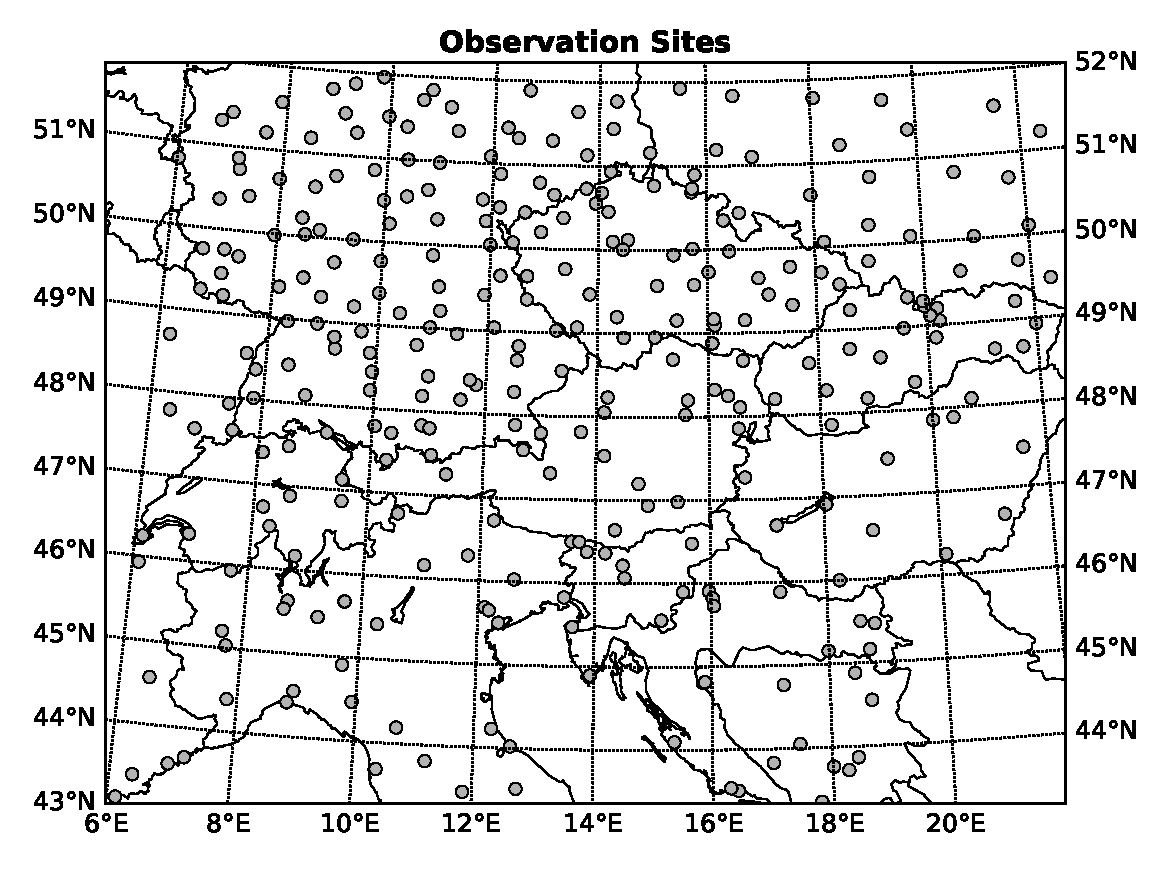
\includegraphics[width=\textwidth ] {graphics/Observation_Sites.eps}
    \caption[Map of Observation Sites]{Model domain and all observation sites where visibility measurements are taken}
    \label{fig:stations}
\end{figure}
 
\subsection{Scores}
For the computations of the scores only certain values on the model domain are used: The model output data for the forecast visibility is a two-dimensional field. For every station where visibility is measured, the data at the point of the coordinates of the measurement station was extracted from the two-dimensional field and evaluated. To obtain values for all coordinates of the stations, a nearest neighbour interpolation was performed. This was done for all points in time, when measurements are taken. Thus, the data can be index by time up to the number of all measurements within the verification period at one location $N_\mathrm{Mes}$ and by location up to the number of considered observations sites $N_\mathrm{S}$. \\
The different scores, we used for the evaluation of the goodness of the visibility prediction, are described in the following.\\

\subsubsection{Root Mean Squared Difference of the Logarithmic values (RMSLog) }
The average of the root-mean-square of the difference of the logarithm of the forecast and observed value is mathematically expressed as the following:
\begin{equation}
    \mathrm{RMSLog}_{n}(\lambda_{\mathrm{lon}}, \phi) =  \frac{1}{N_\mathrm{Mes}}\sum_{m=1}^{N_\mathrm{{Mes}}} \frac{ \sum_{i=1}^{N_{M_\mathrm{{tot}}}} (\log(vis_{\mathrm{o}_{n,m}}) - \log(vis_{\mathrm{f}_{i,n,m}}))^{2}} {N_{M_\mathrm{{tot}}}}
    \label{eq:haselstonerscore_loc}
\end{equation}

\begin{equation}
    \mathrm{RMSLog_{total}}=   \sqrt{\frac{ \sum_{n=1}^{N_\mathrm{S}} \mathrm{RMSLog}_{n} } {N_\mathrm{S}} } \quad .
    \label{eq:haselstonerscore_tot}
\end{equation}
To obtain a local score for each station $\mathrm{RMSLog}_{n}$, first, the average squared differences of the logarithmic values of the forecast visibility $vis_{\mathrm{f}_{i,n,m}}$ and the observed visibility $vis_{\mathrm{o}_{n,m}}$ are calculated. Here $i$ stands for the number of the member, $m$ indexes the time of the $m$th measurement and $n$ the location of the $n$th observation site.
First, the scores are averaged over the whole ensemble, where $N_{M_\mathrm{tot}}$ stands for the total number of ensemble members. Second, the average over all measurements in time is taken, where $N_\mathrm{Mes}$ stands for the number of measurements in the time span of interest.\\
To compute the total score $\mathrm{RMSLog_{total}}$, as described by Equation \eqref{eq:haselstonerscore_tot}, the root-mean-square of the mean of the local score $\mathrm{RMSLog}_{n}$ of the total number of stations $N_\mathrm{S}$ is taken.\\
The score, as described by Equation \eqref{eq:haselstonerscore_tot} and \eqref{eq:haselstonerscore_loc}, is computed from the logarithmic values with respect to the magnitude of the observed values: A forecast value that is off by 20km should be more weighted, when the observed value is 2km than, when it is 70km. Another reason for using a logarithmic score is that the observations are categorized with increasingly large intervals, so this way the different bin sizes of the measurement data (see Table \ref{tab:synoptable}) can be acknowledged.
\\

\subsubsection{Ranked Probability Score (RPS)}
The ranked probability score evaluates the probabilities gained from ensemble forecasting instead of only a mean value \cite{buizza1998impact}. Thus,  it is seen as a more accurate measure to test, if the perturbation scheme is well chosen. It is a commonly used score and described in the following after the textbook by \citeauthor{wilks2011statistical} \cite{wilks2011statistical}.\\
To calculate the RPS, first, the forecast values need to categorized into $K$ different bins. The number of ensemble members $N_{\mathrm{bin}_{j},M}$, whose predicted values are categorized in one bin, needs to be counted for a number of specified points in space and time for all bins. The points are chosen with respect to the available measurements, usually overlapping with their location and timing. As described by Equation \eqref{eq:card_mem}, the condition for a member being included in the count, the forecast values $f$ (in our case $vis_{\mathrm{f}_{i,n,m}}$ ) $\mathrm{bin}_{j,\mathrm{min}} < f < \mathrm{bin}_{j,\mathrm{max}}$ needs to be satisfied.
\begin{equation}
    N_{\mathrm{bin}_{j},M}(\lambda_{\mathrm{lon}}, \phi, t) = | \ \mathrm{mem} : f (\lambda_{\mathrm{lon}}, \phi, t) \in [\mathrm{bin}_{j,\mathrm{min}}, \mathrm{bin}_{j,\mathrm{max}}] \ |
    \label{eq:card_mem}
\end{equation}
From that, the forecast probability of an observation that lies within the interval of the $j$th bin is calculated as
\begin{equation}
 p_{\mathrm{bin}_{j}}(\lambda_{\mathrm{lon}}, \phi, t) = \frac{ N_{\mathrm{bin}_{j},\mathrm{M}} (\lambda_{\mathrm{lon}}, \phi, t)}{ N_{\mathrm{M_{tot}}}} \quad .
\end{equation}
For the RPS, the accumulated probabilities
\begin{equation}
 F_{J}=\sum_{j=1}^{J}  p_{\mathrm{bin}_{j}}
\end{equation}
and accumulated observations
\begin{equation}
 O_{J}=\sum_{j=1}^{J}  o_{\mathrm{bin}_{j}}
\end{equation}
 are used, where $o_{j}$ stands for the occurrence of an event. So if the observed value lies in the interval of the $j$th bin it equals 1, otherwise 0. A consequence of calculating a score from the accumulated probabilities is, that the higher the bin index $j$ is, the less is the accuracy of the bin weighted in the score. Like for the RMSLog, this is a desired property, because the accuracy of the visibility forecasts is more important for low values. Finally, we can define the RPS as
\begin{equation}
    \mathrm{RPS}=\sum_{J=1}^{K} \left( F_{J} - O_{J} \right)^{2} \quad .
    \label{eq:RPS}
\end{equation}
The conditions $ \sum_{j=1}^{K}  p_{\mathrm{bin}_{j}}=1 $ and  $ \sum_{j=1}^{K}  o_{\mathrm{bin}_{j}}=1 $ must hold and consequently, the last term of Equation \eqref{eq:RPS} always vanishes \parencite{wilks2011statistical}.\\
The bin edges for the RPS were defined as: [0.0, 0.5, 1.0, 5.0, 10.0, 15.0, 20.0, 30.0, 50.0, 80.0 ]. The increasing bin size relates to the decrease in accuracy in the number-coded system for the measurement data (Table \ref{tab:synoptable} in Appendix \ref{sec:tabelappendix}).
RMSLog and RPS show a high sensitivity to distance.\\ \\


A major concern when evaluating new parametrizations is, to not assess the performance of the whole model, but only of the parametrization. \\
This problem arises, because for certain days and weathers situations, the forecasts as a whole are bad, and since the visibility forecast uses other model variables as input, the total scores in visibility reflect also the overall model performance. 
The unbiased evaluation of parametrizations can never be achieved to perfection, but a thorough preselection of data can help. For this, the scores can be computed using only data of dates, where the overall model skill was high, or  the correlations of the skill of different model variables and the forecast variable we want to assess can be analysed.\\
Another way to tackle this problem is, to use a relative score. Meaning, if a comparable parametrization already exists, the quality of the forecasts is only quantified in terms of relative improvement.
The Gul-parametrization was so far the only tool for visibility prediction and already implemented in a post-processing package for AROME at ZAMG. Therefore, we decided to evaluate the other parametrizations against the Gul-parametrization (see Table \ref{tab:Paraoverview}).\\
In order to do so, a relative version of the RMSLog and the RPS are introduced. 
For the RMSLog and the RMSE, the relative score is expressed in percentage of the total score of the Gul-parametrization.
For the RPS, the relative version is given by the Ranked Probability Skill Score (RPSS). The RPSS is a traditional skill score. A skill score SS is generally defined as 
\begin{equation}
    \mathrm{SS}=\frac{\mathrm{A}- \mathrm{A_{ref}}}{\mathrm{A_{perf}} - \mathrm{A_{ref}}}
\end{equation}
(e.g. \citeauthor{wilks2011statistical} \cite{wilks2011statistical} ), where A stands for the accuracy. $\mathrm{A_{ref}}$ is the accuracy of the reference case  and $\mathrm{A_{perf}}$ the accuracy of a perfect forecast.
That means that the goodness of the parametrization is rated with respect to a reference parametrization that has a ranked probability score $\mathrm{RPS_{ref}}$. The RPS of the other parametrization is evaluated against it, as described by 
\begin{equation}
    \mathrm{RPSS} = 1 - \frac{\mathrm{RPS}}{\mathrm{RPS}_\mathrm{ref}} \quad ,
    \label{eq:RPS_skill}
\end{equation}
since for the RPS  the perfect accuracy $\mathrm{A_{perf}}$ equals 0. Regarding Equation \eqref{eq:RPS_skill} it is evident that the RPSS has to lie within the interval $[- \infty, \ 1]$ and all values greater than zero indicate a better performance, than the one of the reference. 
\chapter{Results}
\label{sec:results}
In this chapter the findings of this thesis are presented. An inter-comparison of the performance of all implemented parametrizations is shown. Then, the different skills for different scores of the Clark+-parametrization are discussed with respect to the Gul-parametrization, which was used as a reference. In addition, seasonal variations and the influence of the perturbation scheme and the different weather situations on the forecast performance are illustrated and analysed. 

\subsubsection{Overall Performance and Inter-comparison of all Parametrizations }
An overview of the relative average RMSE and RMSLog is provided in Table \ref{tab:scores}. The different scores vary significantly depending on the parametrization and season.\\
Concerning the RMSE for January 2017, presented in Figure \ref{fig:January_RMSE}, four out of seven parametrizations, including the Clark+-parametrization, show a better performance than the reference parametrization (Gul). When comparing this to the RMSLog, presented in Figure \ref{fig:January_logRMSE}, the number decreases to three out of seven, because the Clark+-parametrizations fails by 1\% to outmatch the reference (Table \ref{tab:scores}). These three parametrizations have a worse skill, when evaluated for RMSLog than for RMSE, indicating a decrease in performance for low visibility cases. For the period of July 2016 the overall scores, shown in Figures \ref{fig:July_logRMSE}, \ref{fig:July_RMSE} and \ref{fig: RPS_july} are significantly worse. When analysing the relative RMSLog score in Figure \ref{fig:July_logRMSE}, we cannot find a single parametrization outperforming the Gul-parametrization. Similar can be said for the RMSE (Figure \ref{fig:July_RMSE}). Only the FRAM50-parametrization appears to perform well at first glance, but its poor skill for low visibilities is exhibited by its RMSlog value (Figure \ref{fig:July_logRMSE}) and its RPSS values (Figure \ref{fig: RPS_july}). This seasonal variation is discussed in more detail later in this section.\\
The scores in Table \ref{tab:scores}, show that on average none of the other parametrizations could outperform the Gul-parametrization. Of all implemented parametrizations the Clark+ and FRAMC show the lowest error by 3.75\% and 1.75\%. Although FRAMC has a lower average, we still consider Clark+ as the best alternative to Gul, because its scores show lower overall spread, implying a more stable performance.
\begin{table}[htb]
 \renewcommand{\arraystretch}{2.5}
    \tiny
        \centering
        \begin{tabularx}{\textwidth}{|l |X|X|X|X|X|X|X|}
        \hline
    \textbf{Relative Score}&  \textbf{Clark+}&	\textbf{RUC}	&\textbf{FRAMC}&	\textbf{AIRS}&	\textbf{FRAM5}&	\textbf{FRAM50}&	\textbf{FRAM95}\\
    \hline
    \hline
    \textbf{RMSE July 2016}&	116&	149	&130&	127&	134	&98&	124\\
    \hline
    \textbf{RMSLog July	2016}&102&	140&	116&	114&	121&	136	&155\\
    \hline
    \textbf{RMSE January 2017}&	96&	76&	79&	152&	77&	108&	181\\
    \hline
    \textbf{RMSLog January 2017}&	101&	77&	82&	117&	98&	103&	133\\
    \hline
    \textbf{Average}	&103.75&	110.5&	101.75&	127.5&	107.5&	111.25&	148.25\\
    \hline
    \end{tabularx}
    \caption{Relative Score Overview: the monthly averaged relative RMSE and RMSLog values for all different parametrizations is presented. The Gul-parametrization was used as reference and all values denote the score in percentage with respect to it.}
    \label{tab:scores}
\end{table}
When comparing the RPSS (Figures \ref{fig: RPS_july} and \ref{fig: RPS_jan}) and the RMSLog (Figures \ref{fig:July_logRMSE} and \ref{fig:January_logRMSE}) a strong correlation can be found, since both are weighted scores, as explained in Section \ref{sec:eval}. However, the skill of Clark+ is significantly better, when assessed by the relative RMSLog than by the RPSS. This is probably a result of the different weighting. The RPSS weighting is based on a set of bins, customized to the study of visibility, and is thus, believed to be the more accurate score. Nevertheless, our results show that the verification profits from the usage of different scores. Because although the RPSS is a more sophisticated score, and therefore in the following mainly used for the analysis of the results, error estimation in percentage is easier to understand intuitively.
 
        \begin{figure}[p]
            \centering
            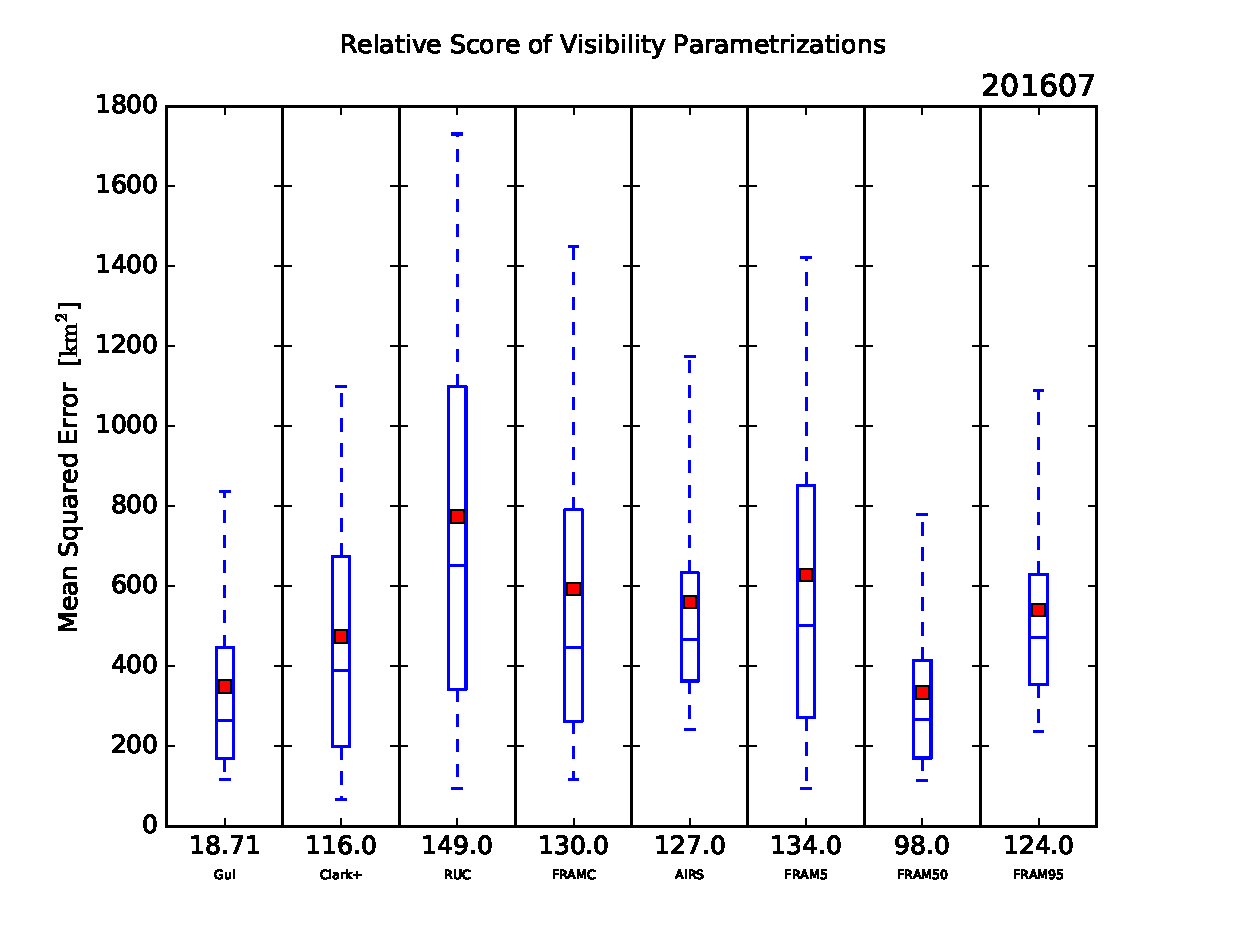
\includegraphics[width=0.8\textwidth]{graphics/results/EnsAv_RMSE_box-201607.eps}
            \caption[Box Plots of MSE, July 2016]{Box plots of the ensemble average Mean Squared Error, average for July 2016. Whiskers denoting the 5th- and the 95th-percentiles, the red squares the mean values. The first value on the X-axis is the average RMSE value of the reference parametrization `Gul' and the other values denote the Root Mean Squared Error relative to the `Gul' parametrization in percentage. }
            \label{fig:July_RMSE}
        \end{figure}

        \begin{figure}[p]
        \centering
            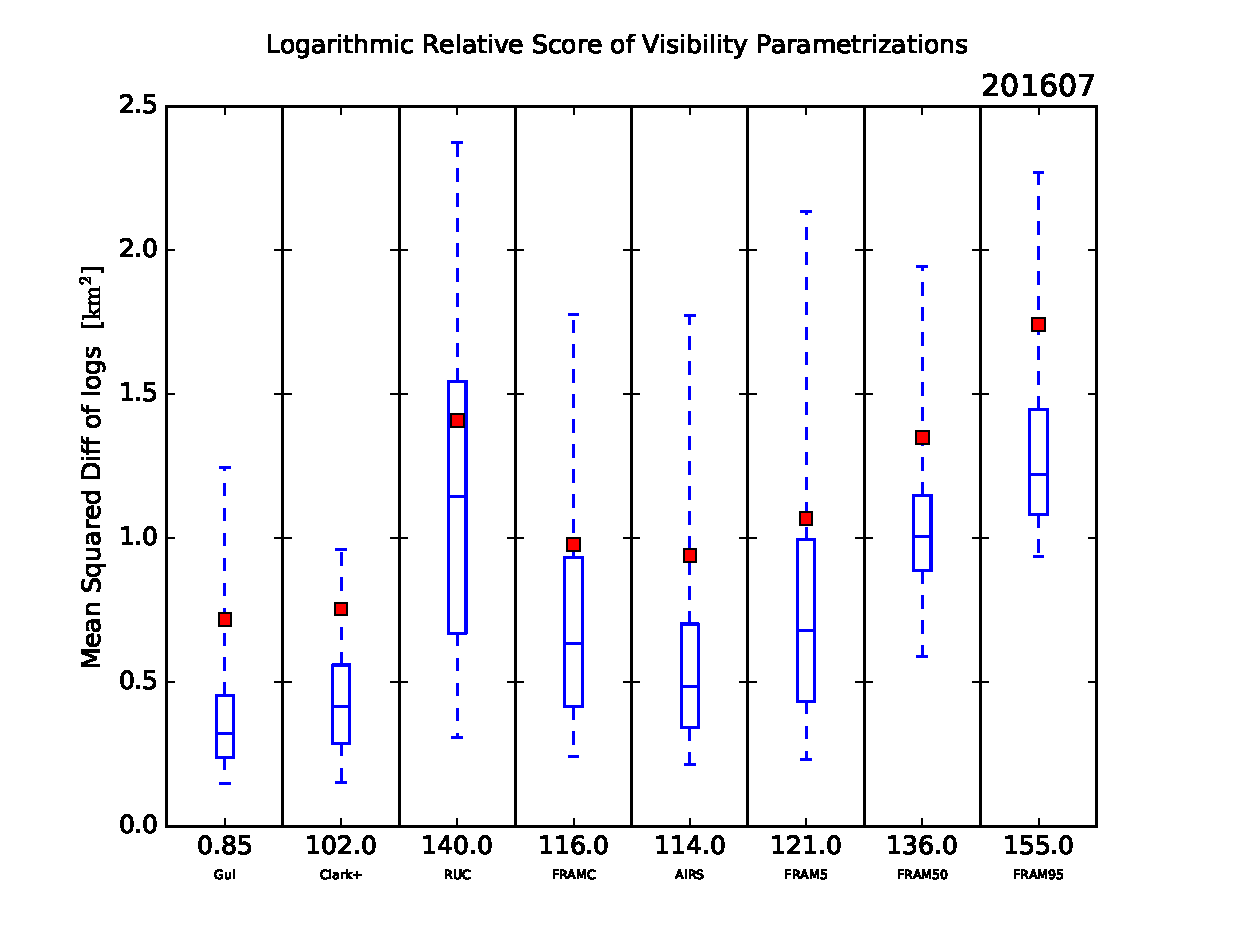
\includegraphics[width=0.8\textwidth]{graphics/results/EnsAv_logRMSE_box-201607.eps}
            \caption[Box Plots of Mean Squared Difference of Logs, July 2016]{Box plots of the ensemble average mean squared difference of the logarithmic observed and forecast values, average for July 2016. Whiskers denoting the 5th- and the 95th-percentiles, the red squares the mean values. The first value on the X-axis is the average RMSLog value of the reference parametrization `Gul' and the other values denote the RMSLog relative to the `Gul' parametrization in percentage.}
            \label{fig:July_logRMSE}
        \end{figure}
\begin{figure}[p]
    \centering
    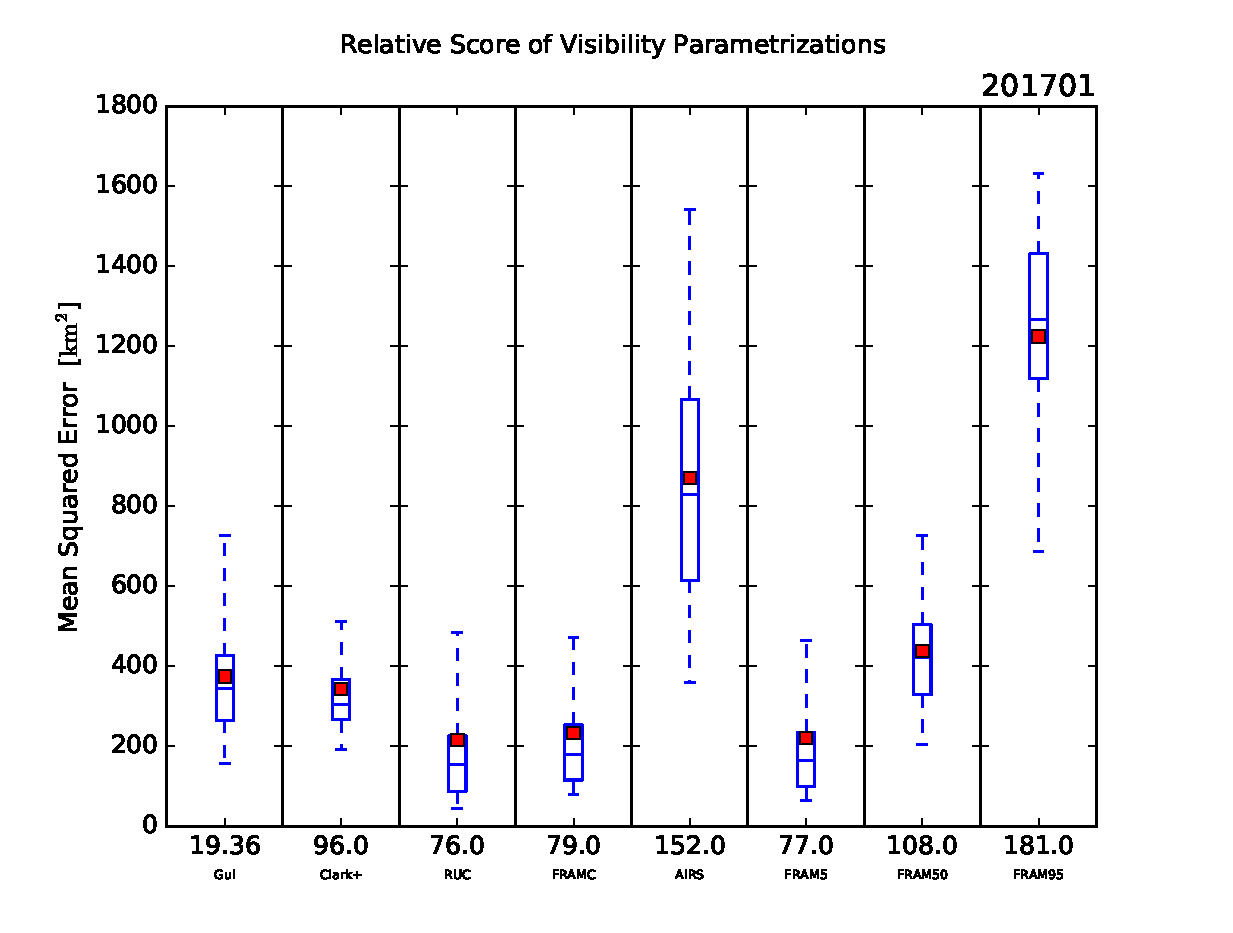
\includegraphics[width=0.8\textwidth]{graphics/results/EnsAv_RMSE_box-201701.eps}
    \caption[Box Plots of MSE, January 2017]{Box plots of the ensemble average Mean Squared Error, average for January 2017. Whiskers denoting the 5th- and the 95th-percentiles, the red squares the mean values. The first value on the X-axis is the average RMSE value of the reference parametrization `Gul' and the other values denote the  Root Mean Squared Error relative to the `Gul' parametrization in percentage.}
    \label{fig:January_RMSE}
\end{figure}
\begin{figure}[p]
    \centering
    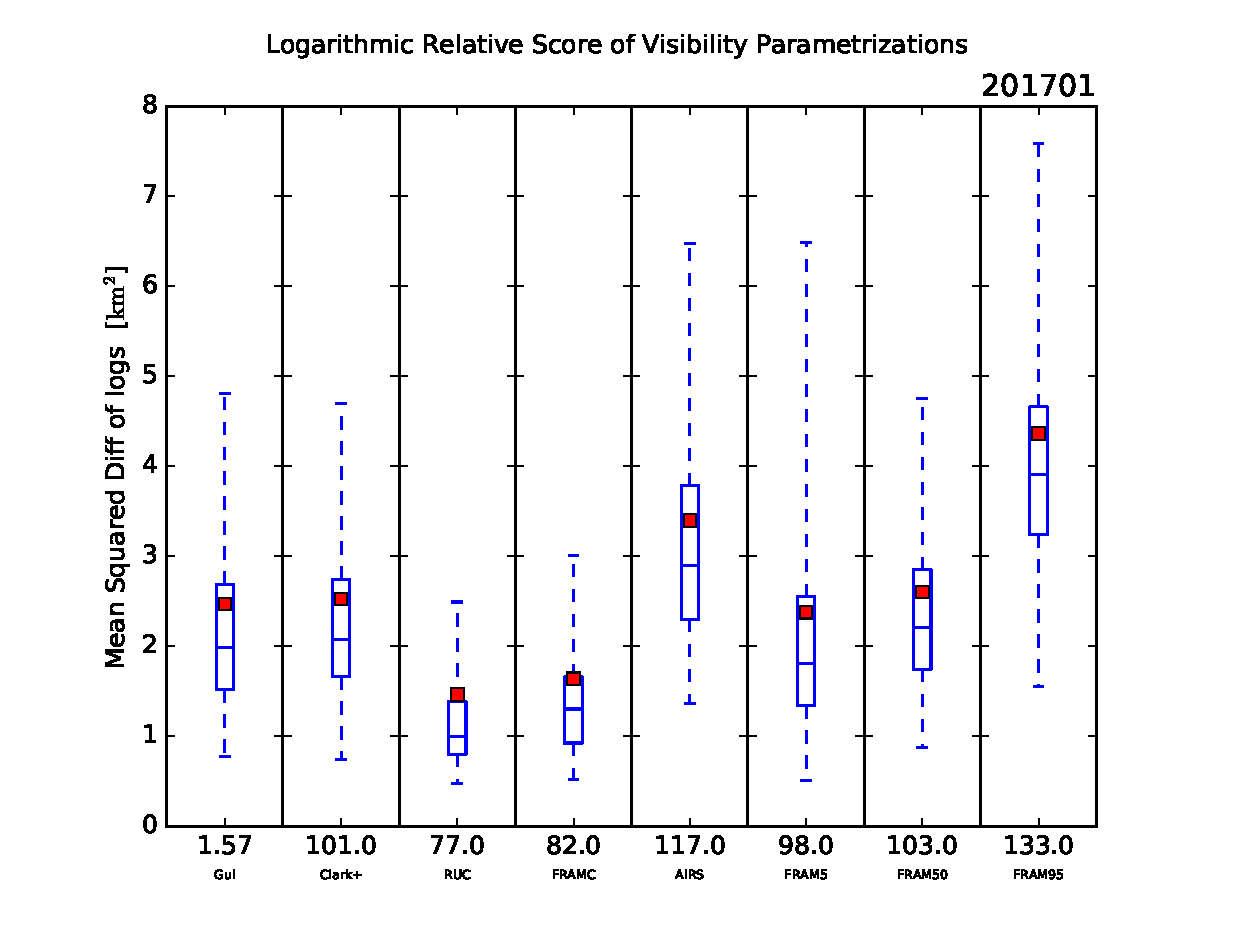
\includegraphics[width=0.8\textwidth]{graphics/results/EnsAv_logRMSE_box-201701.eps}
    \caption[Box Plots of Mean Squared Difference of Logs, January 2017]{Box plots of the ensemble average mean squared difference of the logarithmic observed and forecast values, average for January 2017. Whiskers denoting the 5th- and the 95th-percentiles, the red squares the mean values. The first value on the X-axis is the average RMSLog value of the reference parametrization `Gul' and the other values denote the RMSLog relative to the `Gul' parametrization in percentage.}
    \label{fig:January_logRMSE}
\end{figure}
\FloatBarrier


\subsubsection{Correlation of Weather Conditions and Visibility Forecast}
To understand the correlation of present weather conditions and the forecast visibility, the visibility forecast of $27^{\mathrm{th}}$ January 2017, 09:00 UTC, presented in Figure \ref{fig:cont_vis}, is discussed.\\
As shown in Figure \ref{fig: RPS_jan}, it is one of the days with a comparably high RPSS in the verification period. The satellite image in Figure \ref{fig:Satfoto} is used to analyse the weather conditions. In addition to it, the surface weather analysis in Figure \ref{fig: Bodenkarte06} and \ref{fig: Bodenkarte12} in  Appendix \ref{sec:imagesappendix} provide a qualitative overview for an enhanced interpretation of the correlation of weather conditions and forecast visibility. \\
The local RPSS values of the Clark+-parametrization for $27^{\mathrm{th}}$ January 2017 are shown in Figure \ref{fig:Rated_stations_20170127}.
The good scores in the northern part of the domain are probably the result of the stable and sunny weather conditions. 
The low visibility in some areas like the Austrian-Czech-border is due to fog. In the satellite image (Figure \ref{fig:Satfoto}) fog can be identified as the very homogeneous grey areas. Fog is forecast as liquid cloud water in the model, generally hard to predict and extremely sensitive to initial conditions \cite{zhou2012forecast}. The analysis of the results of days with a particularly good or poor performance revealed a strong correlation between the skill of the  Clark+-visibility-forecast and the skill of the forecast of liquid cloud water close to the surface. Since in this case the fog forecast had a high accuracy, the visibility forecast had a high accuracy as well. Looking at Figure \ref{fig:Satfoto}, \ref{fig: Bodenkarte06} and \ref{fig: Bodenkarte12}, we find a presence of fog in Hungary, where no reduced visibility is indicated in Figure \ref{fig:cont_vis}. The successful prediction for the northeast of Austria and the poor forecast for Hungary are reflected in the local skills illustrated in Figure \ref{fig:Rated_stations_20170127}.
\begin{figure}[h]
    \centering
    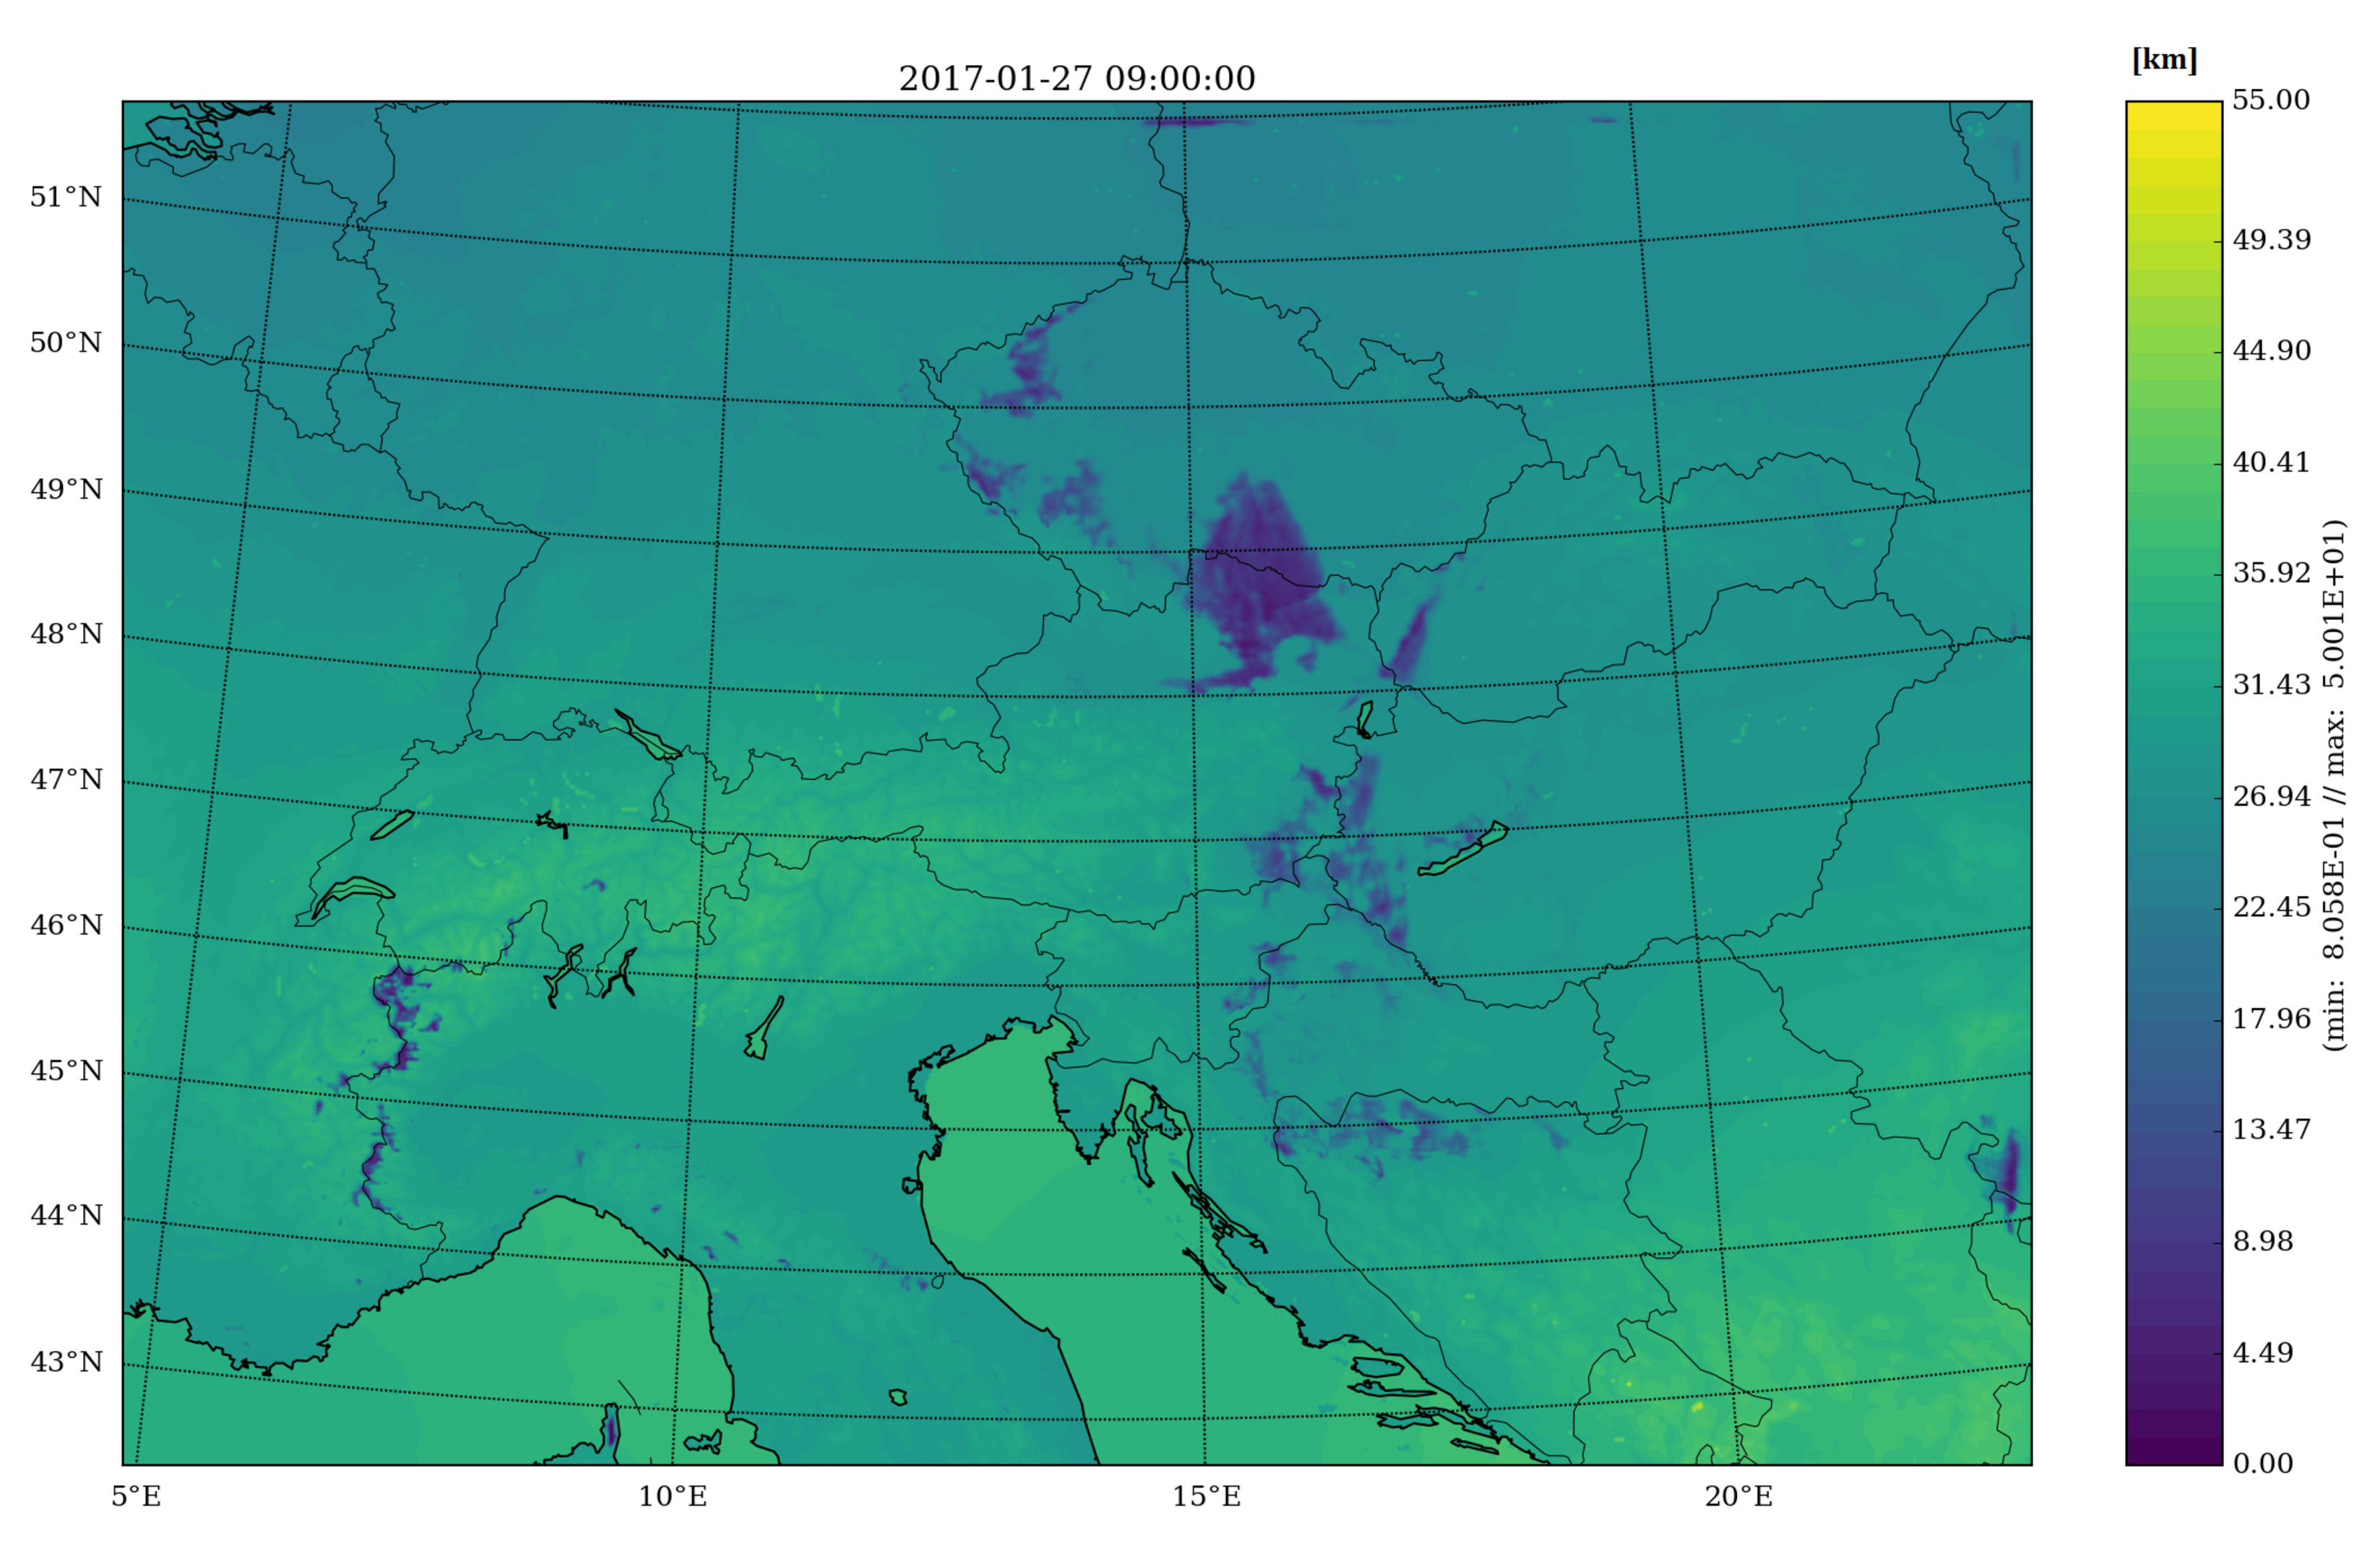
\includegraphics[width=\textwidth]{graphics/visibviri.eps}
    \caption[Contour Plot of Forecast Visibility]{Contour plot of forecast visibility by the Clark+-parametrization on 27-01-2017, 09:00 UTC. The forecast is taken from the control run from the control ensemble. }
    \label{fig:cont_vis}
\end{figure}

\begin{figure}[h]
    \centering
    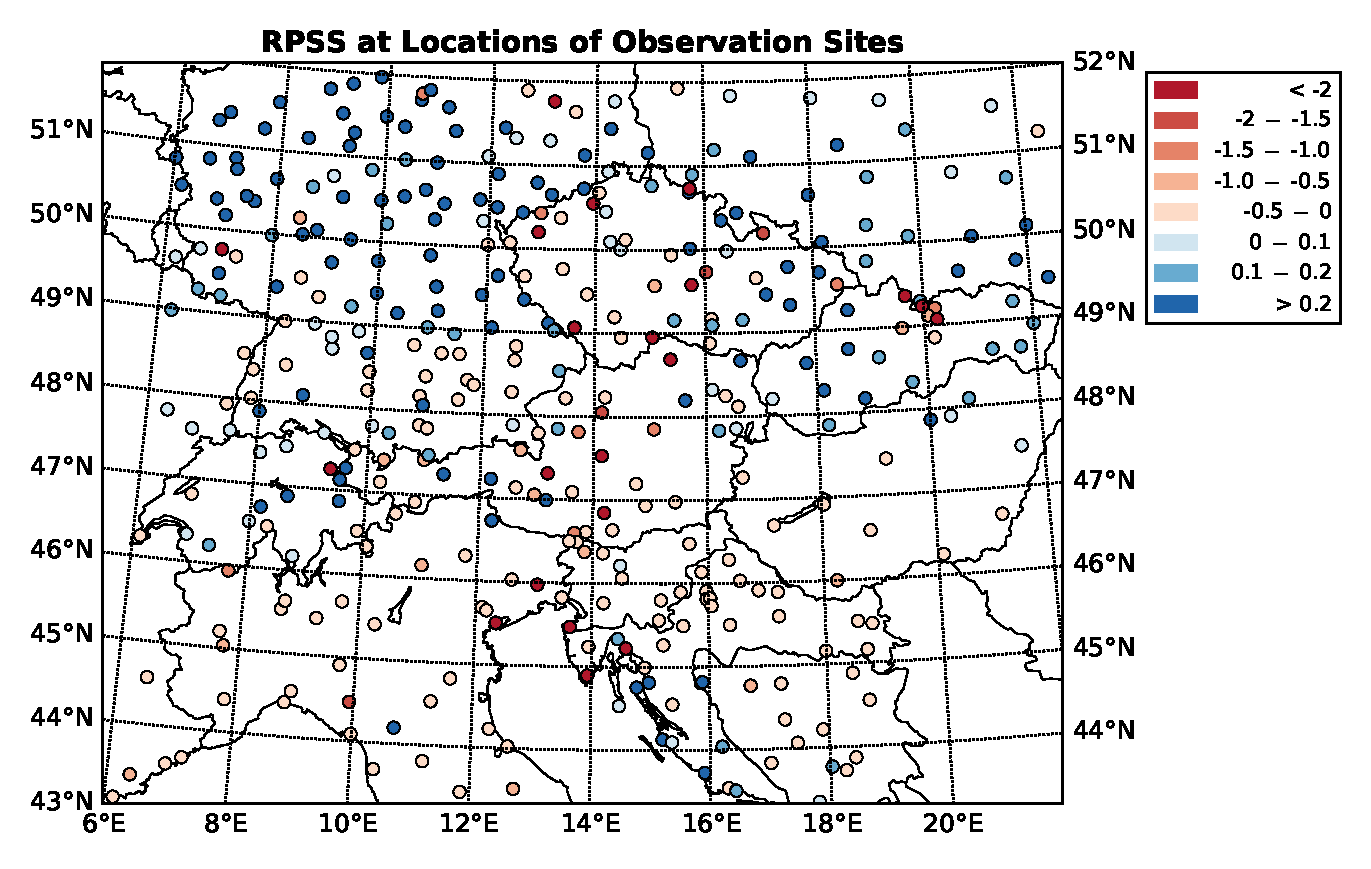
\includegraphics[width=\textwidth]{graphics/results/Rated_stations20170127.eps}
    \caption[Stations Marked with RPSS 27-01-2017]{RPSS of the Clark+-parametrization marked and colour-coded on the considered observation sites on the Austrian AROME  domain on 27-01-2017}
    \label{fig:Rated_stations_20170127}
\end{figure}


\begin{figure}[h]
    \centering
    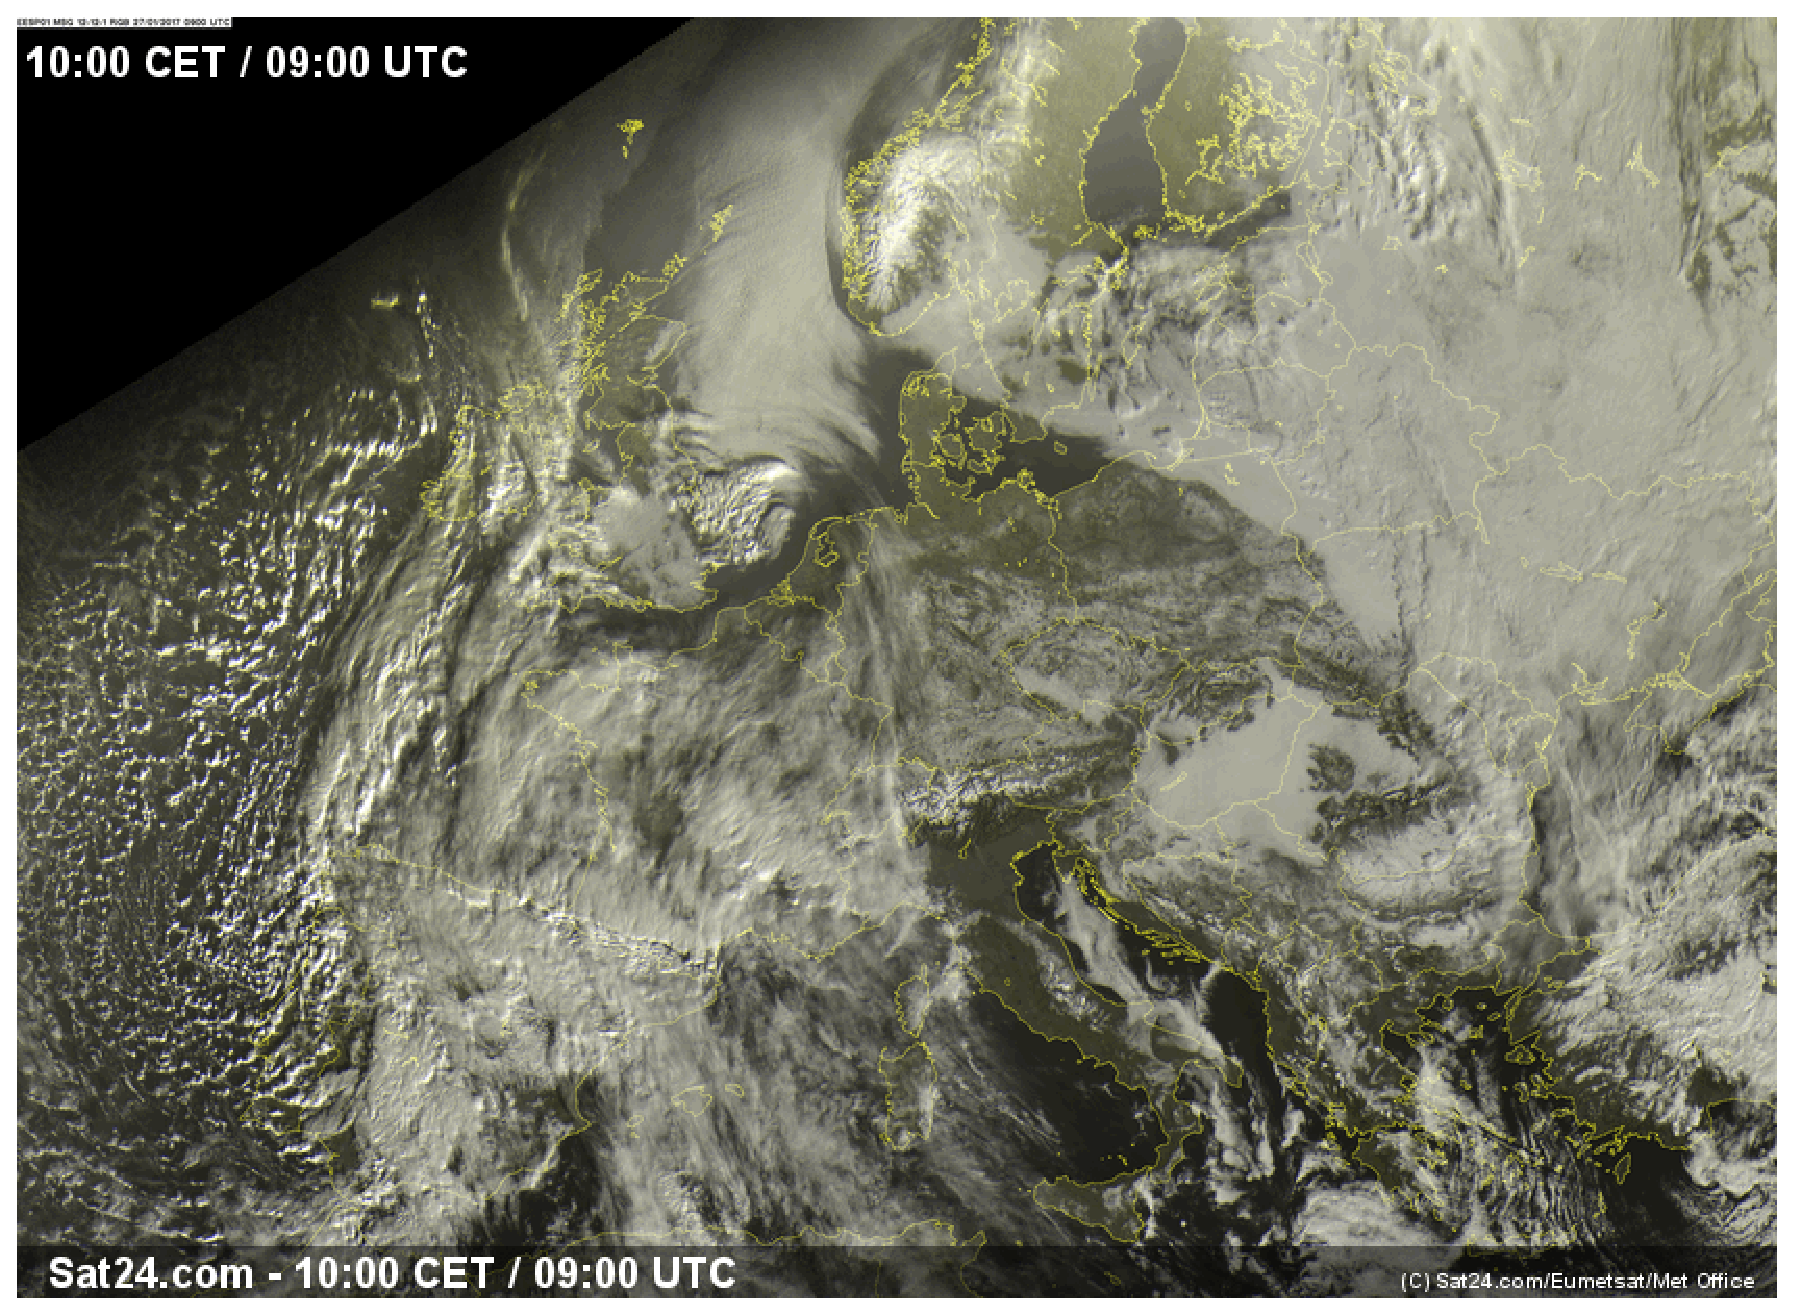
\includegraphics[width=\textwidth]{graphics/sat.eps}
    \caption[Satellite Image 27-01-2017, 09:00 UTC ]{Satellite Image 27-01-2017, 09:00 UTC 27-01-2017, 09:00 UTC of Central Europe. Image from the online archive of `\citeauthor{sat24}' \cite{sat24}}
    \label{fig:Satfoto}
\end{figure}

\FloatBarrier
\subsubsection{Seasonal Variations in Skill}
When comparing Figure \ref{fig: RPS_jan} and Figure \ref{fig: RPS_july} we see a significant difference in skill: The overall RPSS of the Clark+-parametrization is much better in January, whereas the Gul-parametrization seems to be unimpaired by seasonal changes (Figure \ref{fig:July_RMSE}, \ref{fig:July_logRMSE}, \ref{fig:January_RMSE}, \ref{fig:January_logRMSE}). This can be explained by the greater impact of the hydrometeors rain, snow, liquid cloud water and cloud ice in the Clark+-parametrization. In winter, the formation of fog is more likely due to the low saturation humidity.  Moreover, the forecast of precipitation, another parameter that impairs visibility, is more skilful in winter \cite{kidd2012}. This is suspected to be also the cause for the different effects of the perturbations observed in the case studies (Figure \ref{fig:casestudies}). Furthermore, the case studies give reason to believe that if the perturbation scheme is adapted, an increase of the RPSS of about 0.1 in January can be expected. Regarding Figure \ref{fig: RPS_jan}, it can be seen that this would result in the Clark+-parametrization outperforming the Gul-parametrization for most days in winter.\\ 
In summer, on the other hand, the clouds form higher in the atmosphere and the concentration of liquid cloud water is decreased correspondingly. In the lower levels, from which we take the input variables for the visibility module, almost no hydrometeors are present, except for rain in some cases. Although there is a dependency on the relative humidity in the Clark+-parametrization, humidity impacts the visibility only by hygroscopic growth of aerosols. But since climatological aerosol data is used, large discrepancies between the aerosol distributions in the model and the currently present aerosol distributions in the atmosphere can arise. Especially near the coast, the concentration of sea salt can vary strongly in time. Organic matter and sulphates are also effected by hygroscopic growth, but their concentrations are more stable in space and time. 
\begin{landscape}
    \begin{figure}[p]
        \centering
        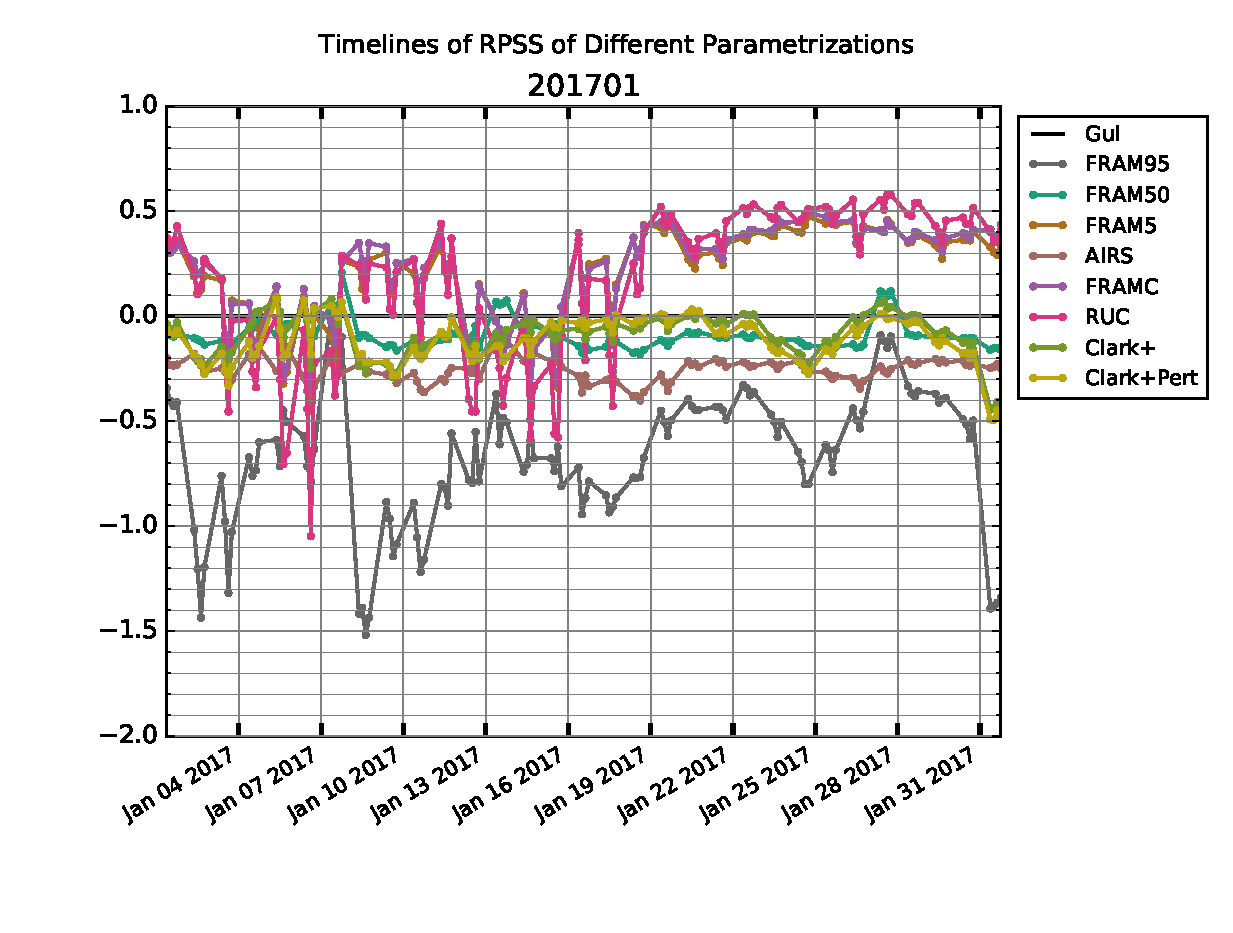
\includegraphics{graphics/results/RPS-201701.eps}
        \caption[Timeline of RPSS for January 2017 ]{RPSS versus time for January 2017. The RPSS of all parametrizations is shown: the unperturbed `Clark+', the totally perturbed `Clark+Pert' and the seven benchmark parametrizations. The black line, always 0, stands for the `Gul'-parametrization, which is the corresponding reference of the RPSS.  }
        \label{fig: RPS_jan}
    \end{figure}
    \begin{figure}[p]
        \centering
        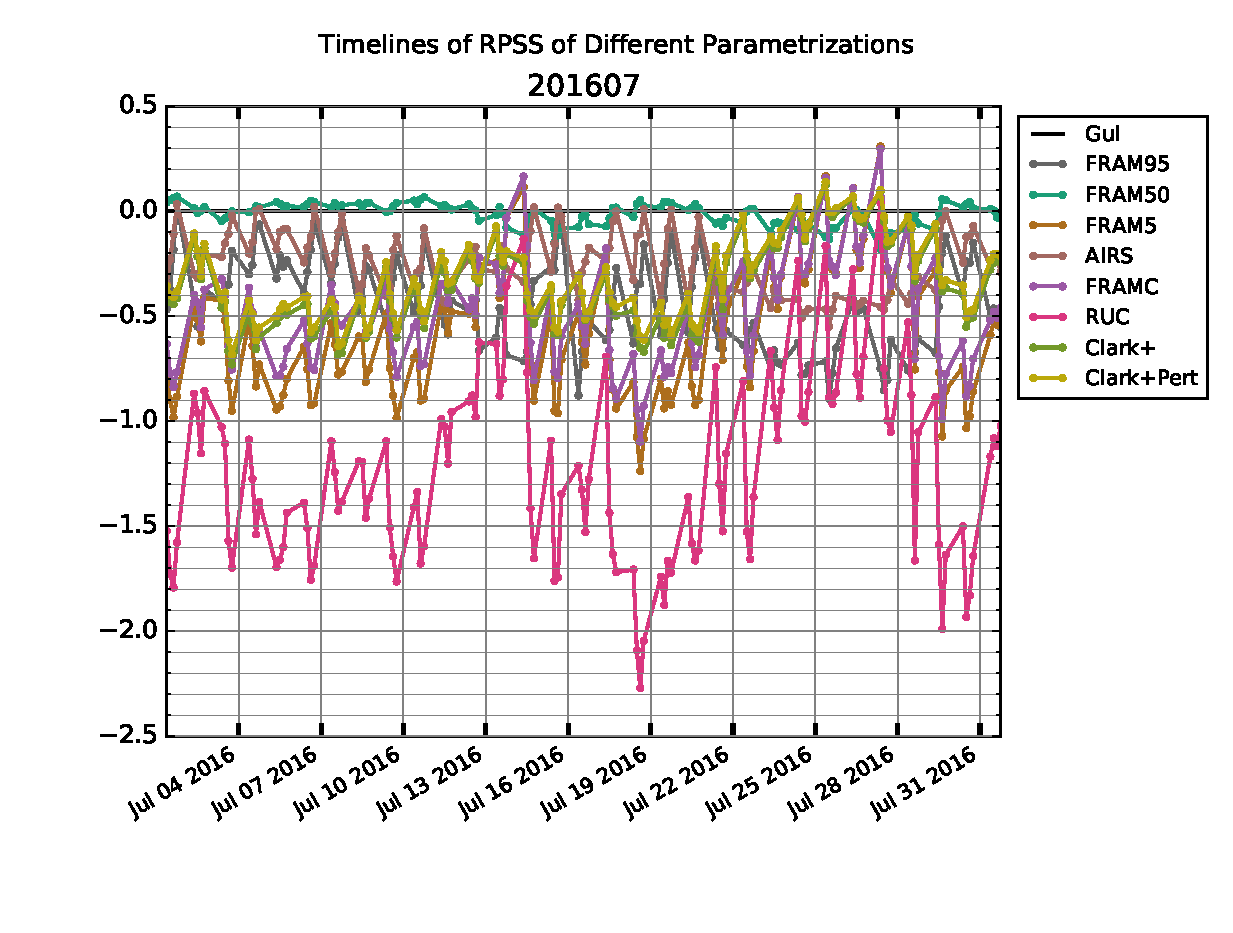
\includegraphics{graphics/results/RPS-201607.eps}
        \caption[Timeline of RPSS for July 2017]{RPSS versus time for July 2016. The RPSS of all parametrizations is shown: the unperturbed `Clark+', the totally perturbed `Clark+Pert' and the seven benchmark parametrizations. The black line, always 0, stands for the `Gul'-parametrization, which is the corresponding reference of the RPSS.}
        \label{fig: RPS_july}
    \end{figure}
\end{landscape}
\FloatBarrier

\subsubsection{Geographical Bias on the Forecast Performance }
When looking at Figure \ref{fig: RPS_jan} and \ref{fig: RPS_july}, it is evident that for some locations the chances of a skilful forecast are higher than for others. Especially along the Adriatic coast, the Clark+-parametrization performs poorly regarding to its RPSS. This is probably, because the Gul-parametrization has a direct dependence on relative humidity, which is a key parameter close to the sea. As mentioned in the discussion of the seasonal bias, sea salt concentration strongly varies, what mainly affects coastal areas. While this is the case along the coast it is noteworthy that locations in landlocked countries like in Austria or the Czech republic profit of the more complex Clark+-parametrization.

\begin{figure}[h]
    \centering
    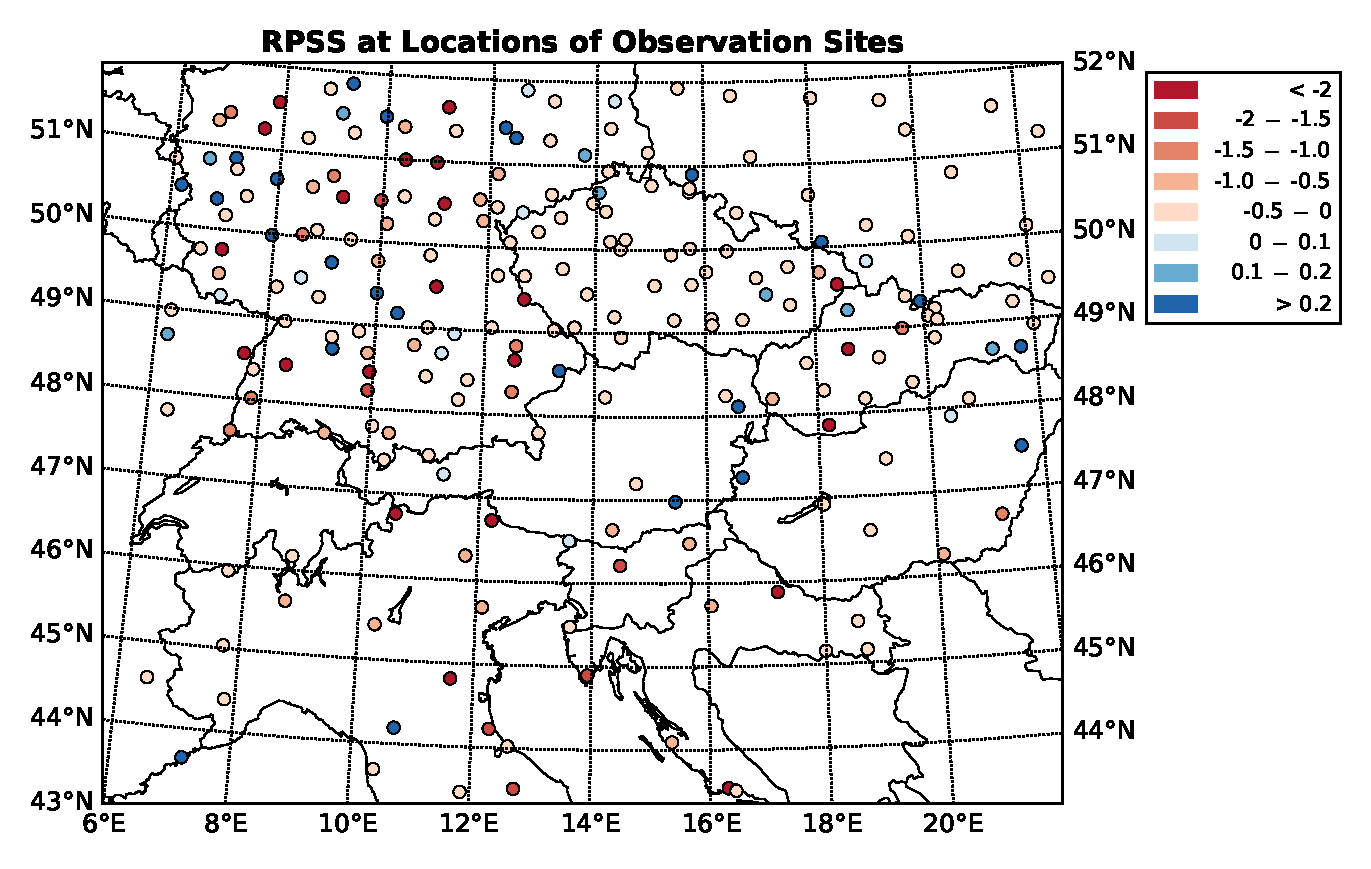
\includegraphics[width=\textwidth]{graphics/results/Rated_stations-201607.eps}
    \caption[Stations Marked with RPSS for July 2017]{RPSS of the Clark+-parametrization marked and colour-coded by value on the considered observation sites on the Austrian AROME domain for July 2016. Only observations sites for which three flawless measurements per day were available were taken into account, and are therefore shown on this plot.}
    \label{fig: Stations_july}
\end{figure}

\begin{figure}[h]
    \centering
    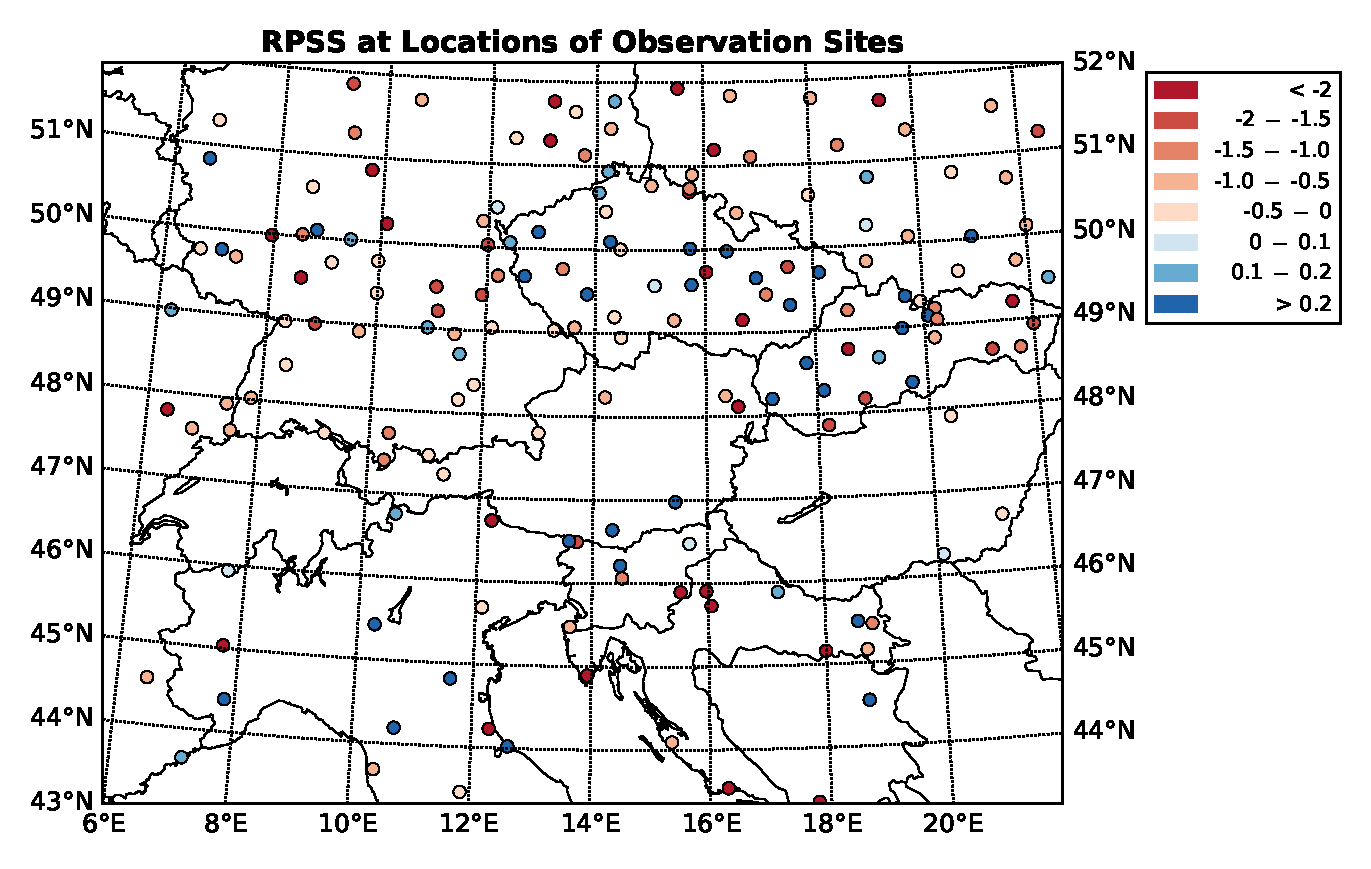
\includegraphics[width=\textwidth]{graphics/results/Rated_stations-201701.eps}
    \caption[Stations Marked with RPSS for January 2017]{RPSS of the Clark+-parametrization marked and colour-coded by value on the considered observation sites on the Austrian AROME domain for January 2017. Only observations sites for which three flawless measurements per day were available were taken into account, and are therefore marked. }
    \label{fig: Stations_jan}
\end{figure}
%\FloatBarrier

\subsubsection{Evaluation of the Perturbation Scheme}
The impact of the different variables can be investigated by analysis of the graphs in Figure \ref{fig:casestudies}. It shows the different RPSS results of the Clark+-parametrization, for the case studies, where different variables and parameters were perturbed, and also the control ensemble, where no additional perturbation was applied. Especially for the test cases in January, significant improvements can be achieved by using a suitable perturbation. But when analysing the data, we find that in some cases the added perturbation can result in a worse skill, than the one of the control ensemble. The exclusive perturbation of the aerosol concentrations `AerPert' is clearly superior to all others on the two days in winter. This was probably induced by very stable weather conditions that led to a better than average predictability of the model. Then, the uncertainties of forecast specific humidity and hydrometeor concentrations go down, but for climatological aerosol data and most constant parameters they remains the same. Figure \ref{fig:casestudies} also reveals that in winter the perturbation of the hydrometeors seems to have a bad effect on the ensemble skill, whereas in summer, it causes the ensemble skill to improve. This is due to the fact that the uncertainty of the forecast concentration of hydrometeors undergoes seasonal variations, because of the different scale of precipitation and cloud formation in winter and summer. In summer small-scale convective processes are much more influential to hydrometeor distributions than in winter  \cite{kidd2012}. \\
Future studies will likely benefit from further development of the local perturbation scheme by adjusting the amplitude of the perturbation to the present situation differently. For this study monthly climatological extrema were used to set the perturbation amplitude for each month, but the seasonally differing dynamics of precipitation, like its scale and velocities, were neglected. The major difficulty for incorporating them lies within the determination of the adjustment factor, which would require further investigation to be set properly.\\
Regarding the test cases in July, on the other hand, the totally perturbed ensemble, `TotPert', outperforms all others on average. We suspect that this behaviour is due to a greater contribution of small-scale processes  to the overall atmospheric state in summer than in winter, so the increased uncertainties let the model profit from a perturbation \cite{kidd2012}. When comparing the different single perturbations with the total perturbation, the total perturbation seems well balanced, although the perturbation of hydrometeors has clearly the strongest effect, since we can observe a significant correlation between the two ensembles.\\
The perturbation of the specific humidity always decreased the skill, except for two measurements in July, where it had no measurable effect. This is thought to be the result of an overestimation of uncertainty for the specific humidity. The specific humidity seems to be already forecast quite well by the model, which also leads to the good skill of the Gul-parametrization. \\ \\
Furthermore, the results presented in Figure \ref{fig:casestudies} show, that even a locally applied perturbation scheme can lead to more skilful ensemble forecasts and can be an alternative in cases, where a global perturbation scheme cannot be implemented. Although this was only tested for the visibility parametrization, there is no obvious reason why this should not be generalized for different parametrizations and model components.
\begin{figure}[h]
    \centering
    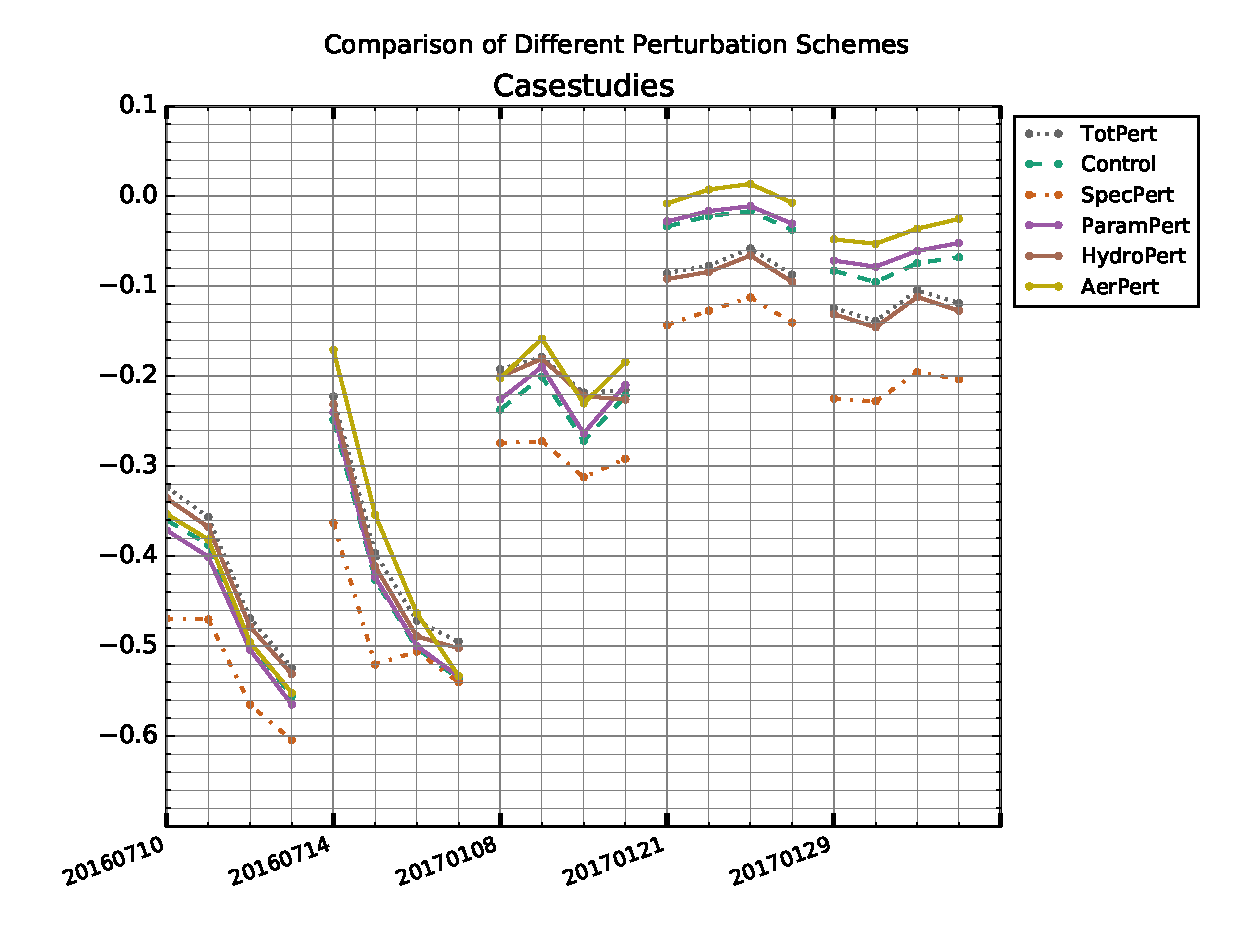
\includegraphics[width=\textwidth]{graphics/results/RPS-Casestudies.eps}
    \caption[Case studies of Different Perturbation Schemes]{RPSS  of the Clark+-parametrization for five dates in July 2016 and January 2017: the label positions of the on the x-axes indicates the skill score corresponding to the 09:00 UTC measurements and the other three following up  to 12:00, 15:00 and 18:00 UTC. The x-axes is linear for each day, but the time-frame where no measurements are taken is cut out. }
    \label{fig:casestudies}
\end{figure}
\FloatBarrier


\chapter{Conclusion and Outlook}
\label{sec:con_n_out}
Although the overall performance of the established Gul-parametrization is in most cases better than of the newly introduced one, we have reason to believe, that with the general advancement of the model, the explicit Clark+ visibility forecast will be able to outmatch it in the future. On the long run the overall improvement of AROME and in particular prognostic aerosols and advances in data assimilation should provide a decrease of the uncertainties and approximations, which are mainly responsible for the rather low scores of the Clark+-parametrization.\\ \\
Unfortunately, including data assimilation, would have exceeded the scope of this Master's thesis and was therefore not done. Data assimilation mainly improves forecasts within the first few hours. Since the outputs used in the evaluation were taken the earliest after nine hours of forecast duration, we suspect that data assimilation would not have had any effects.
However, for short-range forecasts data assimilation reduces uncertainties and thus, can lead to different results for the skill of the visibility parametrization, because of the increased accuracy of relative humidity and hydrometeor concentrations. It seems likely, that data assimilation would have a major influence on how well a certain perturbation scheme performs too. Especially within the first two hours, the uncertainties of some quantities decrease, whereas of others, e.g. aerosol distribution, they remain the same. As a consequence the ranges of the perturbation patterns will need to be adapted, if data assimilation is used. Testing the effect of data assimilation on the performance in short-range forecasts should be the subject of future studies, to investigate, if the new visibility parametrization can profit from it and might be used in nowcasting systems (NWP within six hours from base time). \\ \\
The results confirm that the severest weakness of our set-up is that the used aerosol data is climatological. Thus, more exceptional events, e.g. sudden increase of Saharan dust over Europe and the like, are not treated in the model. Also changes in the distribution of sea salt, which heavily contributes to the total aerosol concentration in coastal areas and varies strongly, is neglected. Since the new parametrization
relies heavily on aerosols, it is thought to provide significant improvement in performance if a prognostic aerosols scheme would be used. This is further confirmed by the large increase in ensemble skill, when aerosols are included in the perturbation scheme, as shown in the case studies. Tests with aerosol data from a high resolution aerosol transport model were run and also showed promising results. These tests were carried out by a different implementation of the parametrization in a python program that used AROME output and the mentioned aerosol data as input. The aerosol transport model is based on the weather research and forecasting (WRF) model and has not been coupled with AROME so far. Coupling them could be a way to incorporate high quality aerosol forecasts in the model, but is challenging for the operational mode due to the associated computational costs.
For the operational mode the MESO-NH package, which is partially used in AROME and open-source, already includes a simple prognostic aerosol scheme that could be harmonized and calibrated for use in the AROME model in future studies.  \\ \\
A change that is expected to improve the parametrization itself is, to not only consider the forecast visual range at the current location, but also at the adjacent grid points. This would lower the discrepancy of forecast and observation, because the human observers also analyse all directions, when taking measurements. But because of  how the model domain is split up for parallelization purposes, we were not able to implement this in the current version. It might be worth considering implementing such a method as  part of the post-processing of the output data. Similar techniques are already applied to probabilistic precipitation forecasts \cite{theis_hense_damrath_2005}\\ \\
Concerning the perturbation scheme, we found that a local perturbation can be a good strategy to introduce a more realistic spread for model parts or parametrizations, when global perturbations cannot be applied to the needed extent. This is not limited to the forecast of visibility, but can be applied to other forecast variables as well.
Especially when the model parts of interest have a large number of different complex dependencies, it is in many cases not feasible to implement a global perturbation of the corresponding quantities. Then local perturbation can help to still be able to obtain an estimate of reliability and the probability distribution of the forecast variable. \\
Another advantage of a local perturbation scheme is that for diagnostic quantities like visibility it can also be used in post-processing, if the prediction is not contained in the model. The perturbation scheme could also be further improved by fine tuning the set-up and a better pattern generator. \\
As illustrated and discussed in Chapter \ref{sec:results}, the perturbation of specific humidity resulted in a decrease of overall skill. Hence, decreasing the perturbation range drastically or simply excluding specific humidity from the perturbation scheme, is expected to increase the skill of the totally perturbed ensemble. It should also lead to a stronger correlation of the totally perturbed ensemble and the perturbed aerosol and the perturbed parameter ensemble, which seem the most promising indicated by their high overall performance, especially in winter.\\ \\
The severe shortcomings of the pattern generator, discussed in Section \ref{sec:pattern gen}, are briefly revised:  Due to the fact that the namelist settings cannot be directly related to spatial scales, scaling the perturbations is a process of trial and error. Additionally, the cut-off of sampled values distorts the probability density functions. This could be resolved by re-sampling values that lie outside the range.
Solving these issues is challenging, but worth it, since any future experiments that include perturbations would profit from it.

\newpage\printbibliography[heading=bibintoc,
title={Bibliography}
]
\newpage
\section*{Statement of Originality}
\hfill \break
\hfill \break

I, Magdalena Elisabeth Haselsteiner, born on 27.05.1992 in Korneuburg, hereby declare in front of Freie Universität Berlin that I have written the present Master's thesis independently without the use of sources and aids other than those specified. The present work has not been submitted to any other university in this or similar form and has not been published yet.\hfill \break
\hfill \break
\hfill \break
\hfill \break
\hfill \break
\hfill \break
Magdalena Elisabeth Haselsteiner

\newpage


\section*{Acknowledgements}
Firstly, I want to express my sincere gratitude to all members of the  `model development'-group at `Zentralanstalt f\"ur Meteorologie und Geodynamik' and in particular to my scientific supervisor Dr. Clemens Wastl. Everyone in the department  was incredibly patient, especially with my initial lack of knowledge in meteorology, offering insightful explanations and great support. \\
Florian Weidle and Florian Meier helped me a lot to get on with the peculiarities of using the high performance computer at the ECMWF and Josef Kemetmüller was never tired of demystifying the underlying mathematics of the model for me. Moreover, I am grateful to have had the opportunity to profit from Jasmin Vural's experience and her advice on scientific writing. Thanks to them, but also to Christoph Wittmann and Clemens Wastl, I felt welcome at the department from day one.\\
Dr. Wastl's door was always open and he helped me to stay on track during my research phase, without interfering too much, letting me create a work based on my own ideas.\\ \\
I would also like to acknowledge Prof. Roland Netz at Free University of Berlin and Mag. Christoph Wittmann and Dr. Yong Wang at ZAMG for making this cooperation possible and letting me carry out this thesis in the form as it is.\\ \\
Finally, I want to thank my family for their support throughout my studies, especially my brother Andreas Haselsteiner. He was not only always willing to discuss the topics of my research, but also to help in times of struggle of more personal nature.\\
Special thanks goes to all my dear friends, in particular to Clemens Heistracher and Christa Lichtenberger, who have always been a source of encouragement, even when being on the other side of the globe.
Without you, my studies, including working on this thesis, wouldn't have been half as much fun and as successful, thanks to our shared studying sessions and the sometimes badly needed distractions.

\newpage
\appendix
\chapter{Tables}
\label{sec:tabelappendix}
 \section{Set-Up of Perturbation}
\begin{longtable}[H]{|l|c|c|c|}
    \hline 
    \multicolumn{4}{|l|}{\textbf{Perturbation settings}}\\
    \hline 
    \textbf{Variable} & \textbf{spatial correlation [km]} & \textbf{distribution} & \textbf{scaling factor} \\ 
    \hline
    $c_{ice}$ & 60000 & lognormal & 0.25 \\
    \hline
    $c_{snow}$ & 60000 & lognormal & 0.25 \\
    \hline
    $c_{rain}$ & 60000 & lognormal & 0.25 \\
    \hline
    $c_{lcw}$ & 60000 & lognormal & 0.25 \\
    \hline

    $c_{\mathrm{om}}$ &200000  & lognormal& Table \ref{tab:scale_aerosol} \\
    \hline
    $c_{\mathrm{bc}}$ & 200000  &lognormal & Table \ref{tab:scale_aerosol} \\
    \hline
    $c_{\mathrm{ss}}$ & 200000  & lognormal & Table \ref{tab:scale_aerosol} \\
    \hline
    $c_{\mathrm{sul}}$ & 200000  & lognormal & Table \ref{tab:scale_aerosol} \\
    \hline
    $c_{\mathrm{dd}}$ & 200000 &  lognormal &Table \ref{tab:scale_aerosol}  \\
    \hline
    $q_{\mathrm{spec}}$ & 60000  & normal & 2.00 \\
    \hline
    $\alpha_{\mathrm{om}}$ &60000  & normal&  1.00\\
    \hline
    $\alpha_{\mathrm{bc}}$ & 60000  &normal & 1.00 \\
    \hline
    $\alpha_{\mathrm{ss}}$ & 60000  & normal &  1.00\\
    \hline
    $\alpha_{\mathrm{sul}}$ & 60000  & normal & 1.00 \\
    \hline
    $\alpha_{\mathrm{dd}}$ & 60000  & normal & 1.00 \\
    \hline
    $\sigma_{\mathrm{om}}$ &60000  & normal& 0.1\\
    \hline
    $\sigma_{\mathrm{bc}}$ & 60000  &normal & 0.1\\
    \hline
    $\sigma_{\mathrm{ss}}$ & 60000  & normal &  0.1\\
    \hline
    $\sigma_{\mathrm{sul}}$ & 60000  & normal & 0.1\\
    \hline
    $\sigma_{\mathrm{dd}}$ & 60000  & normal & 0.1 \\
    \hline
    $c_{\mathrm{0,rain}}$ & 60000  & normal & 0.20 \\
    \hline
     $c_{\mathrm{0,lcw}}$ & 60000  & normal & 0.20 \\
    \hline
     $c_{\mathrm{0,ice}}$ & 60000  & normal & 0.20 \\
    \hline
     $c_{\mathrm{0,snow}}$ & 60000  & normal & 0.20 \\
    \hline
    $c_{\mathrm{1,rain}}$ & 60000  & normal & 0.20 \\
    \hline
     $c_{\mathrm{1,lcw}}$ & 60000  & normal & 0.20 \\
    \hline
     $c_{\mathrm{1,ice}}$ & 60000  & normal & 0.20 \\
    \hline
     $c_{\mathrm{1,snow}}$ & 60000  & normal & 0.20 \\
    \hline
     

    \caption{Namelist settings defining the patterns, constructed by the pattern generator, of the perturbed quantities. The spatial correlation provided, is only a namelist setting and has a complex relation to the actual spatial scale as described in Section \ref{sec:pattern gen}. It cannot be directly related with a length scale, because it is scaled with respect to the Earth's radius, since it as originally set-up for a global model. \label{tab:namelist_pert}}
\end{longtable}

\begin{landscape}
    \begin{longtable}{|l|c|c|c|c|c|c|c|c|c|c|c|c|}
            \hline 
            \multicolumn{13}{|c|}{  \textbf{Scaling Factors of Aerosol Perturbation} }\\
            \hline 
                   
              \textbf{Month}&\textbf{1}&\textbf{2}&\textbf{3}&\textbf{4}&\textbf{5}&\textbf{6}&\textbf{7}&\textbf{8}&\textbf{9}&\textbf{10}&\textbf{11}&\textbf{12}\\
            \hline 
            \hline
            Sulphate&1.3357& 1.5475 & 2.1818 & 2.8114 & 2.7717 &  3.1702 & 3.6221 & 3.4091 & 3.6193 & 3.0257 & 3.9347 & 4.4281 \\
            \hline
            Organic Matter & 4.3013 & 4.2449 & 4.0527 & 3.6794 &  4.3204 &  4.4870 & 3.7650 & 3.3974 & 3.0685 & 3.3869 & 3.5936 & 4.0124\\
            \hline
            Sea Salt&3.6922 & 3.3340 & 2.2834 & 2.0473 & 1.5699 &  1.4266 &  1.8392 & 1.7394 & 2.3499 & 2.7272 & 3.5206 & 3.1504 \\
            \hline
            Desert Dust& 3.4771 & 2.2858 & 2.5117 & 3.4750 &  4.1395 & 4.0536 & 3.5781 & 3.6066 & 3.9279 & 3.1142 &  2.4776 & 2.4406\\
            \hline
            Black Carbon &  5.2838&  5.3458 & 5.0817 & 4.7262 & 5.4137 & 5.6549 & 4.7267 & 4.2958 & 3.9782 & 4.2889 & 4.5131 & 4.9752 \\
            \hline
    \caption{Scaling factors  \label{tab:scale_aerosol} of the different aerosols. Set with respect to their global maxima}
    \end{longtable}
\end{landscape}

\section{Variables and Abbreviations}

\begin{longtable}[H]{|l|c|c|}
\hline 
\multicolumn{3}{|l|}{\textbf{Used Variables}}\\
\hline 
\textbf{Variable} &\textbf{Name} & \textbf{Unit} \\ 


\hline
$A$ & non-parametrized tendency & varies\\
\hline
$a_{0,i}$, $a_{1,i}$ & surface volume coefficients & $ \left[ \mathrm{ m^{2} \ kg^{-1}} \right]$, [none] \\
    \hline
$a^{s}_{n}$, $b^{s}_{n}$ & Mie coefficients& [none]\\
\hline
$B_{a}$ &brightness of the object& $ \left[ \mathrm{cd \ m^{-2}} \right] $\\
\hline
$B_{b}$ &brightness of the background & $ \left[ \mathrm{cd\  m^{-2}} \right] $\\
\hline
$B_{s}$ &brightness of scattered light & $ \left[ \mathrm{cd\  m^{-2}} \right] $\\
\hline
$c_{\mathrm{bc}}$ &mass concentration of black carbon & $ \left[ \mathrm{\mu g \ kg^{-1}} \right] $\\
\hline 
$C_{ext}$ &extinction cross section & $ \left[ \mathrm{m^{2}} \right] $\\
\hline
$c_{j}$ &constant parameters & varies\\
\hline 
$c_{\mathrm{ice}}$ &mass concentration of ice & $\left[\mathrm{ kg \ kg^{-1} }\right]$\\
\hline
$c_{\mathrm{lcw}}$ &mass concentration of liquid cloud water&$\left[\mathrm{ kg \ kg^{-1} }\right]$\\
\hline
$C$ & Contrast &[none]\\
\hline
$C_{p}$ &specific heat of air for constant pressure&[$\mathrm{ kg\ m^{2}\ 
K^{-1} s^{-2} }$]\\
\hline
$c_{\mathrm{snow}}$ &mass concentration of snow & $\left[\mathrm{ kg \ kg^{-1} }\right]$\\
\hline
$c_{\mathrm{rain}}$ &mass concentration of rain &$\left[\mathrm{ kg \ kg^{-1} }\right]$\\
\hline
$c_{\mathrm{om}}$ &mass concentration of organic matter & $ \left[ \mathrm{\mu g \ kg^{-1}} \right] $\\
\hline
$c_{\mathrm{ss}}$ &mass concentration of sea salt &  $ \left[ \mathrm{\mu g \ kg^{-1}} \right] $\\
\hline
$c_{\mathrm{sul}}$ &mass concentration of sulphates &  $ \left[ \mathrm{\mu g \ kg^{-1}} \right] $\\
\hline
$c_{\mathrm{dd}}$ &mass concentration of desert dust &  $ \left[ \mathrm{\mu g \ kg^{-1}} \right] $\\
\hline
$E$ & electric field vector &  [$\mathrm{V \ m^{-1}}$] \\
\hline
$\vec{e}_{r}$ &radial unit vector &  $ [ \mathrm{none}] $\\
\hline
${e}_{j}$ & prognostic model variabels &  varies\\
\hline
$\vec{F}$&dissipative forcing&[$\mathrm{kg \ m^{-1} s^{-2}}$]\\
\hline
$g$&gravitational constant&[$\mathrm{kg \ m^{-1} s^{-2}}$]\\
\hline
G&geometric factor& $ \left[ \mathrm{m^{2}} \right] $\\
\hline

$L_{\Psi}$& spatial correlation length&[km]\\
\hline
$m$ &zonal wave number& [none]\\
\hline
$M$ &source/sink term for humidity& $\left[\mathrm{ kg \ kg^{-1} \ s^{-1} }\right]$\\
\hline
$n$ &total wave number& [none]\\
\hline
$T$ &temperature& [$^{\circ}$ K]\\
\hline
$T_{x}$ &tendency of  x & varies\\
\hline
$p$ & pressure & [Pa] \\
\hline
$P$ &parametrized tendency & varies\\
\hline
$P_{x}$ &perturbation of  x & varies\\
\hline
$Q$ &heat& [J]\\
\hline
$ Q_{ext}$&extinction coefficient& [none]\\
\hline
$q_{\mathrm{rel}}$ &relative humidity& [none]\\
\hline
$q_{\mathrm{spec}}$ &specific humidity&$\left[\mathrm{ kg \ kg^{-1} }\right]$\\
\hline
$r$ &particle radius& [m]\\
\hline
$\vec{r}$ & radial vector& $ [m]$\\
\hline
$r_{j}$ &random number& [none]\\
\hline
$R$ &gas constant& $ \left[\mathrm{ kg \ m^{2}s^{-2} \ K^{-1} \ mol^{-1}} \right]$\\
\hline
$R_{\mathrm{E}}$ &average radius of the Earth& [km]\\
\hline
RPS &Ranked Probability Score & [none] \\
\hline
RPSS &Ranked Probability Skill Score & [none] \\
\hline
$s$ &scaling factor & [none] \\
\hline
SS &Skill Score & [none] \\
\hline
$t$ &time & [sec] \\
\hline
$\vec{v}$ & wind velocity& $\left[\mathrm{ m \ s^{-1} }\right]$\\
\hline
$\vec{V}$ & horizontal wind vector& $\left[\mathrm{ m \ s^{-1} }\right]$\\
\hline
$vv_{\mathrm{score}}$ &model score &[km]\\
\hline
$vis_{\mathrm{o}_{n}}$ & observed visibility value& [km]\\
\hline
$vis_{\mathrm{f}_{n}}$ &forecast visibility value &[km]\\
\hline
$z$ & height &[m]\\
\hline
$w$ & vertical wind component& $\left[\mathrm{ m \ s^{-1} }\right]$\\
\hline
$\alpha$ & scattering size parameter &[none]\\
\hline
$\alpha_{j}$ & attenuation coefficient of aerosols&$\left[\mathrm{ m^{2} \ g^{-1} }\right]$\\
\hline
$\beta_{\mathrm{a},j}$ & atmospheric extinction coefficient &[$\mathrm{km^{-1}}$]\\
     & of different aerosols &     \\
\hline
$\beta_{h,i}$ & atmospheric extinction coefficient  &[$\mathrm{km^{-1}}$]\\
& of different hydrometeors &\\
\hline
$\beta_{R}$ & atmospheric extinction coefficient  &[$\mathrm{km^{-1}}$]\\
& by Rayleigh scattering &\\
\hline
$\beta_{\mathrm{tot}}$ & atmospheric extinction coefficient&[$\mathrm{m^{-1}}$]\\
\hline
$\varepsilon$ &liminal contrast&[none]\\
\hline
$\kappa$ & Poisson constant & $\left[\mathrm{ mol^{-1} }\right]$\\
\hline
$\rho$ &density of air& $\left[\mathrm{ kg\ m^{-3} }\right]$\\
\hline
$\rho_{dry}$ &density of dry air& $\left[\mathrm{ kg\ m^{-3} }\right]$\\
\hline
$\sigma_{j}$ & scattering cross section of aerosols&$\left[\mathrm{ m^{2} }\right]$\\
\hline
$\lambda$ & wavelength & [m]\\
\hline
$\vec{\lambda}$ & Lyapunov vector& [$s^{-1}$]\\
\hline
$\lambda_{j}$ & Lyapunov exponent& [$s^{-1}$]\\
\hline
$\lambda_{\mathrm{lon}}$ & longitude & [$^{\circ}$]\\
\hline
$\phi$ & latitude &[$^{\circ}$]\\
\hline
$\Phi$ & geopotential &$\left[\mathrm{ m ^{2}\ s^{-2} }\right]$\\
\hline
$\Phi_{\mathrm{t}}$ & time dependent phase factor &[none]\\
\hline
$\vec{\Omega}$ & angular velocity & [none]\\
\hline
$\vec{\omega}$ & vorticity & [$s^{-1}$]\\
\hline

\caption{List of used variables \label{tab: variables}}
\end{longtable}

\begin{table}[h]
    \footnotesize
    \centering
        \begin{tabular}{|l|c|}
        \hline
        \textbf{Abbreviation and Symbols}&\textbf{Meaning}\\
        \hline
        \hline
        AROME&Application of Research to Operations on Mesoscale\\
        \hline
        ALADIN& Aire Limitée Adaptation Dynamique Développement International\\
        \hline
        ECMWF& European Centre for Medium-Range Weather Forecasts\\
        \hline
        EDA & Ensemble Data Assimilation\\
        \hline
        FFT & Fast Fourier Transformation\\
        \hline
        IFS&Integrated Forecast System \\
        \hline
        LAM&Limited Area Model \\
        \hline
        NWP & Numerical Weather Prediction\\
        \hline
        UTC & Universal Time, Coordinated\\
        \hline
        RMSE& Root Mean Squared Error\\
        \hline
        RMSLog & Root Mean Squared Difference of the Logarithmic values\\
        \hline
        RPS & Ranked Probability Score\\
        \hline
        RPSS & Ranked Probability Skill Score\\
        \hline
        WMO& World Meteorological Organization\\
        \hline
        WRF& Weather Research and Forecasting\\
        \hline
        $\Im$ & Imaginary part of a complex number\\
        \hline
        $\Re$ & Real part of a complex number\\
        \hline
        
    
    \end{tabular}
    \caption{List of abbreviations and symbols in this thesis}
    \label{tab:abbrivitations}
\end{table}

\begin{table}[h]
    \footnotesize
    \centering
        \begin{tabular}{|l|c|}
        \hline
        \textbf{SYNOP key}&\textbf{visibility [km]}\\
        \hline
0	& 0.00\\
\hline
1&	0.10\\
\hline
2 &  0.20\\
\hline
...& ..\\
\hline
49 & 4.90\\
\hline
50&	5.00\\
\hline
51&	none\\
\hline
...& ..\\
\hline
55& none\\
\hline
56&	6.00\\
\hline
57&	7.00\\
\hline
...& ..\\
\hline
79&	29.00\\
\hline
80&	30.00\\
\hline
81&	35.00\\
\hline
...& ..\\
\hline
88&	70.00\\
\hline
89&	more than 70\\
\hline

    \end{tabular}
    \caption{SYNOP keys: Numeric system used by the human observers to encode visibility}
    \label{tab:synoptable}
\end{table}

\chapter{Images}
\label{sec:imagesappendix}
\section{Surface Weather Analysis}
\begin{figure}[H]
    \centering
    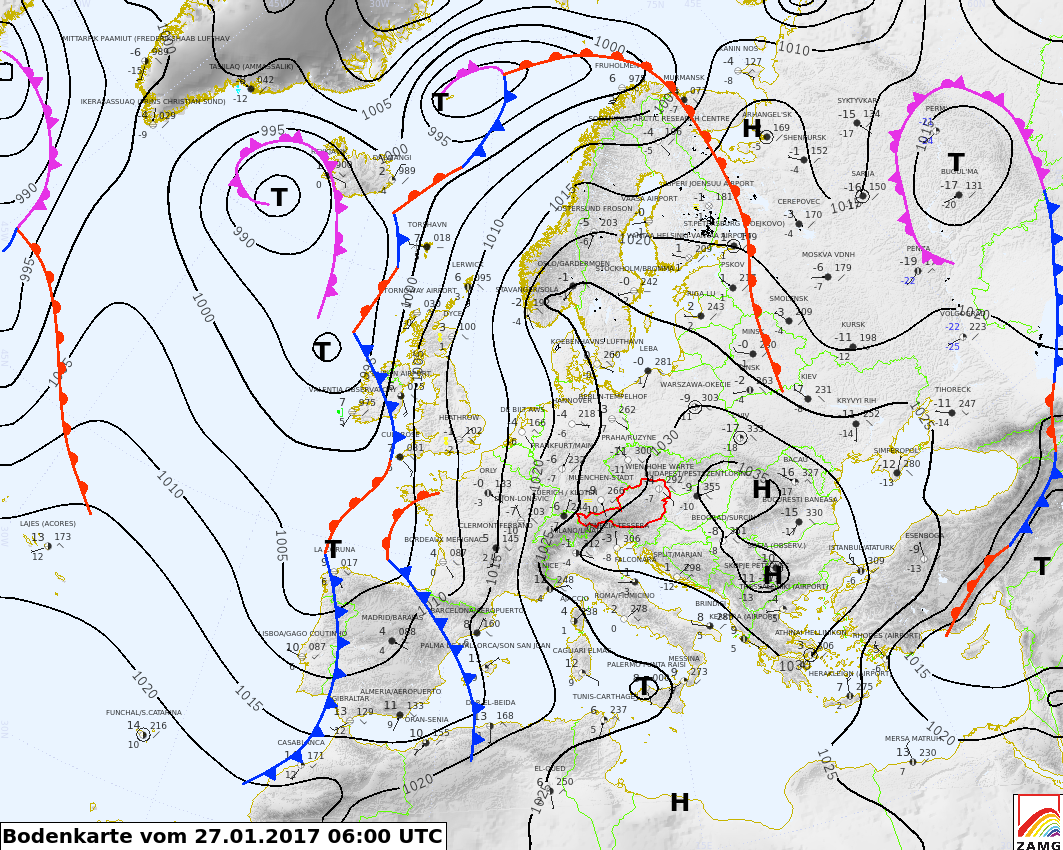
\includegraphics[width=\textwidth]{graphics/Bodenkarte0600.png}
    \caption[Surface Weather Analysis 06:00 UTC]{Surface weather analysis 27-01-2017, 06:00 UTC of Europe. Image from the online archive of `\citeauthor{zamg}'  \cite{zamg}.}
    \label{fig: Bodenkarte06}
\end{figure}

\begin{figure}[H]
    \centering
    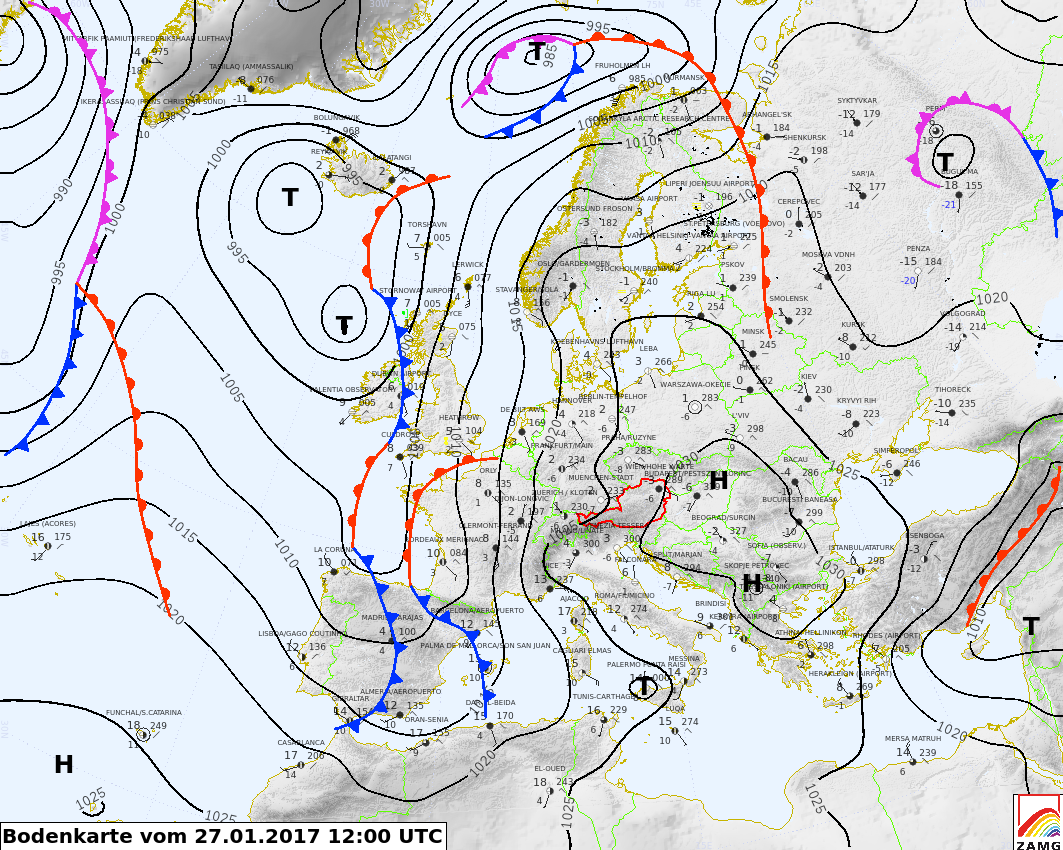
\includegraphics[width=\textwidth]{graphics/Bodenkarte1200.png}
    \caption[Surface Weather Analysis 12:00 UTC]{Surface weather analysis 27-01-2017, 12:00 UTC of Europe. Image from the online archive of `\citeauthor{zamg}'  \cite{zamg}.}
    \label{fig: Bodenkarte12}
\end{figure}
\setlength{\bibitemsep}{1em}


\end{document}
